\documentclass[Master, ngerman, UKenglish]{scrbook}
%------------------------------------------------------------------------------
% This file contains a skeleton thesis for
% a Physics or Astronomy Institute in the University of Bonn

% Specify the thesis type as an option: PhD, Master, Diplom, Bachelor
% Specify the thesis stage as an option: Draft (default), Submit, Final, PILibrary

% Specify the language(s) in the class and then use babel.
% If you need more than one language, give the default language last,
% e.g. ngerman, UKenglish for a thesis in British (UK) English where you want
% to be able to set the language to German for some part of it.

%------------------------------------------------------------------------------
% Pass TeX Live version to the package
% Use command pdflatex --version to find out which version you are running
% Add option backref=false when your thesis is ready to turn off back-referencing
% in your bibliography
\usepackage[texlive=2016,backref=false]{ubonn-thesis}
% Adjustments to standard biblatex style
\usepackage{ubonn-biblatex}
\usepackage{float}
\usepackage[export]{adjustbox}
\usepackage[margin=1in]{geometry}
\usepackage{lineno}
\usepackage{enumitem}

% Glossary package
% \usepackage[acronym,toc,nosuper]{glossaries}
% TikZ packages and libraries
% \usepackage{tikz}
% \usepackage{tikz-3dplot}
% \usepackage{pgfplots}
% \usetikzlibrary{positioning,shapes,arrows}
% \usetikzlibrary{decorations.pathmorphing}
% \usetikzlibrary{decorations.markings}
\usepackage{thesis_defs}
\newcommand{\uproman}[1]{\uppercase\expandafter{\romannumeral#1}}
\setlength\parindent{0pt}

%------------------------------------------------------------------------------
% Instead of colouring  links, cites, table of contents etc.
% put them in a coloured box for the screen version.
% This is probably a good idea when you print your thesis.
% \hypersetup{colorlinks=false,
%   linkbordercolor=blue,citebordercolor=magenta,urlbordercolor=darkgreen
% }

%------------------------------------------------------------------------------
% When writing your thesis it is often helpful to have the date and
% time in the output file. Comment this out for the final version.
%\ifoot[\today{} \thistime]{\today{} \thistime}

% In order to check if your labels are referenced try the refcheck package
% \usepackage{refcheck}

%------------------------------------------------------------------------------
% biblatex is included by ubonn-thesis. Look there for the settings used.
% See the options for settings that can be changed easily.
% For further changes copy the \RequirePackage[...]{biblatex} here
% and include ubonn-thesis with the option biblatex=false.

% Specify the bibliography files here and not at the end!
% Use standard_refs-bibtex if you use bibtex or bibtex8
% and standard_refs-biber  if you use biber
\addbibresource{bib/thesis_refs.bib}
\addbibresource{bib/standard_refs-biber.bib}

%------------------------------------------------------------------------------
% The following definitions are used to produce the title pages
% needed at various stages
\newcommand{\thesistitle}{Improving Four-Top-Quark Event Classification with Deep Learning Techniques using ATLAS Simulation}
\newcommand*{\thesisauthor}{Niklas W. Schwan}
\newcommand*{\thesistown}{Place of birth}
\renewcommand*{\InstituteName}{\PI}
\renewcommand*{\inInstitute}{\inPI}
\renewcommand*{\InstituteAddress}{\PIaddress}
% Adjust \thesisreferee...text depending on male/female referee
\newcommand*{\thesisrefereeonetext}{1.\ Gutachter}
\newcommand*{\thesisrefereeone}{Prof. \ Dr.\ Markus Cristinziani}
\newcommand*{\thesisrefereetwotext}{2.\ Gutachterin}
\newcommand*{\thesisrefereetwo}{Prof.\ Dr.\ Florian Bernlochner}
% Date when thesis was submitted (Master/Diplom)
% Year or Month, Year when thesis was submitted (PhD)
\newcommand*{\thesissubmit}{XX.YY.2020}
% \newcommand*{\thesissubmit}{Month 2020}
% Date of thesis examination (PhD)
\newcommand*{\thesispromotion}{XX.YY.2020}
% Month and year of the final printed version of the thesis
\newcommand*{\thesismonth}{November}
\newcommand*{\thesisyear}{2020}
\newcommand*{\thesisnumber}{BONN-IR-2020-XXX}

%------------------------------------------------------------------------------
% The abstract is only needed for the printed version and should be in
% English regardless of the language of the thesis
\newcommand{\thesisabstract}{%
  \begin{otherlanguage}{UKenglish}
    This is your thesis abstract. It may be in a language that is
    different from the rest of your thesis.
  \end{otherlanguage}
}

%------------------------------------------------------------------------------
% \includeonly can be used to select which chapters you want to process
% A simple \include command just inserts a \clearpage before and after the file
% Note that \includeonly can be quite picky! Do not forget to put a
% comma after the filename, otherwise it will simply be ignored!
% \includeonly{%
%   thesis_intro,
%   thesis_appendix,
%   thesis_acknowledge
% }

%------------------------------------------------------------------------------
% Give a list of directories where figures can be found. Do not leave
% any spaces in the list and end the directory name with a /
\graphicspath{%
  {figs/}%
  {figs/cover/}%
}

%------------------------------------------------------------------------------
% Make a glossary and a list of acronyms
% \makeglossaries

% Glossary entries
% \input{thesis_glossary}

% Draft version - add the word DRAFT on the cover pages
\ifthenelse{\equal{\ThesisVersion}{Draft}}{%
  \usepackage{background}
  \ifthenelse{\texlive < 2013}{%
    \SetBgContents{DRAFT}
    \SetBgColor{blue!30}
  }{%
    \backgroundsetup{contents=DRAFT, color=blue!30}
  }
}

\ifthenelse{\equal{\ThesisVersion}{Draft}}{%
  \ifthenelse{\texlive < 2013}{%
    \SetBgContents{}
  }{%
    \backgroundsetup{contents={}}
  }
}{}

%------------------------------------------------------------------------------
\begin{document}

% Cover page of thesis - this is only needed for the printed final
% version to be submitted to the department library
% Do not use this page for thesis submission to the Prüfungsamt or Promotionsbüro!
\ifthenelse{\equal{\ThesisVersion}{PILibrary}}{%
  \typeout{Document \jobname, Info: PI library version of thesis}
  \input{../cover/\ThesisType_Cover}
}{}

% Start counting pages from the title page
\frontmatter
% Dedication has to come before \maketitle
% \dedication{Dedicated to no one}

% Select the correct title page(s)
\ifthenelse{\equal{\ThesisType}{Unknown}}{%
  \typeout{Document \jobname, Error: Unknown thesis type - no title page printed}
}{%
  % Bachelor thesis only has one title page
  \ifthenelse{\equal{\ThesisType}{Bachelor}}{%
    \typeout{Document \jobname, Info: Bachelor thesis}
    \input{../cover/\ThesisType_Title}
  }{%
    \ifthenelse{\equal{\ThesisVersion}{Final} \OR \equal{\ThesisVersion}{PILibrary}}{%
      % Final and PI library versions
      \typeout{Document \jobname, Info: Final version of a \ThesisType  thesis}
      \input{../cover/\ThesisType_Final_Title}
    }{% Submission and draft versions
      \input{../cover/\ThesisType_Submit_Title}
      \typeout{Document \jobname, Info: Draft/submission version of a \ThesisType  thesis}
    }
  }
}

\pagestyle{scrplain}

%------------------------------------------------------------------------------
% You can add your acknowledgements here - don't forget to also add
% them to \includeonly above
%------------------------------------------------------------------------------
\chapter*{Acknowledgements}
\label{sec:ack}
%------------------------------------------------------------------------------

I would like to thank ...

You should probably use \texttt{\textbackslash chapter*} for
acknowledgements at the beginning of a thesis and
\texttt{\textbackslash chapter} for the end.

%%% Local Variables: 
%%% mode: latex
%%% TeX-master: "../mythesis"
%%% End: 


\tableofcontents

\mainmatter
\pagestyle{scrheadings}

% Turn off DRAFT for the following pages
\ifthenelse{\equal{\ThesisVersion}{Draft}}{%
  \ifthenelse{\texlive < 2013}{%
    \SetBgContents{}
  }{%
    \backgroundsetup{contents={}}
  }
}{}

%------------------------------------------------------------------------------
% Add your chapters here - don't forget to also add them to \includeonly above
%\linenumbers		% line numbers!!! uncommend in the end
%==============================================================================
\chapter{Introduction}
\label{sec:intro}
%==============================================================================

Leukipp (450–370 B.C.) and Demokrit (460–371 B.C.) were most likely the first humans that postulated that matter is composed of indivisible objects. Even though our knowledge about matter has been greatly improved ever since then, the fundamental statement still holds up. Our current understanding of the elementary particles and fundamental forces in our universe is described by the Standard Model of particle physics (SM). It is the unification of many profound theoretical ideas which are capable of explaining almost all observed phenomena. \\
The SM's heaviest elementary particle is the top quark with a mass close to that of a gold atom. Due to its high mass, plays the top quark a special role in the search for beyond the Standard Model physics. When four top quarks are produced in a single proton-proton collision with an energy of over $\SI{700}{GeV}$, they create the heaviest particle final state ever seen at any particle collider. The simultaneous production of four top quarks is an incredibly rare process which makes it interesting to study and hard to observe. Reason enough to investigate this process with new techniques such as Deep Neural Networks. \\
Deep Neural Networks are the models used in deep learning which over the passed decade has developed to most flexible and widely applied machine learning field. In recent years Deep Neural Networks have become the go-to machine learning technique for speech recognition, spam filters, self driving cars and many other applications. With the high Luminosity upgrade of the Large Hadron Collider the number of observed events will increase largely. Making Deep Neural Networks which performance scale very well with the amount of available data to the very promising prospect. \\
This thesis uses the four-top-quark process as a framework to investigate how suitable Deep Neural Networks are for event classification for rare processes. Feedforward Neural Networks will be used to investigate both the achievable performance and the dominant and hard to distinguishing backgrounds. Recurrent Neural Networks with raw kinematic information will be used to investigate if the Neural Network can construct better features than humas can. For better rejection of backgrounds, which are hard to distinguish from the four-top-quark process, a hadronic top quark reconstruction is carried out. \\
The chapters are organized as follows: Chapter \ref{sec:theory} briefly introduces the Standard Model of particle physics and the four-top-quark production. In Chapter \ref{sec:ATLAS}, a short overview of the Large Hadron Collider and the ATLAS experiment is given. The utilized datasets and their simulation is discussed in Chapter \ref{sec:Samples}. Chapter \ref{sec:Deep_learning} gives a brief introduction to deep learning and different types of Neural Networks. The setup up as well as the first studies of Neural Networks are introduced in Chapter \ref{sec:NNSetup}. The last chapter (Chapter \ref{sec:Results}) presents the results of the Neural Network studies and a reconstruction of hadronically decaying top quarks. \\
The terminology of particles physics and deep learning is different. For instance are datasets commonly called samples and features variables. In this thesis the phrase coming from deep learing will be used unless a physics concept is introduced. For obvious reasons will the instances of data be called \textit{events}.


%==============================================================================
\chapter{Theoretical Background}
\label{sec:theory}
%==============================================================================
This chapter will introduce the basic theoretical knowledge needed for the analysis carried out in the following chapters. First, a short overview of the Standard Model of particle physics is given, discussing the fundamental particles and their interactions. Special emphasis is put on the top quark as its properties are pivotal for the four-top-quark process studied in this thesis. The final state and the production channels of the four-top-quark process will be described in the last section of this chapter. \\
It is not common to use S.I. units in elementary particle physics energy, mass and, momenta scales encountered are tiny. The system used instate is known as natural units where [kg,m,s] are replaced by [$\hbar$,$c$,GeV\footnote{GeV is the abbreviation for Giga electron volt where $1\text{eV} = 1.602 \cdot 10^{-19}$ J}]. To simplify the units $\hbar = c = 1$ will be used in this thesis. Thus, all momenta, energies, and masses have the same unit GeV whereas time, and length are given in terms of GeV$^{-1}$.

\section{The Standard Model of Particle Physics}
\label{sec:SM}
\begin{figure}[H]
\centering
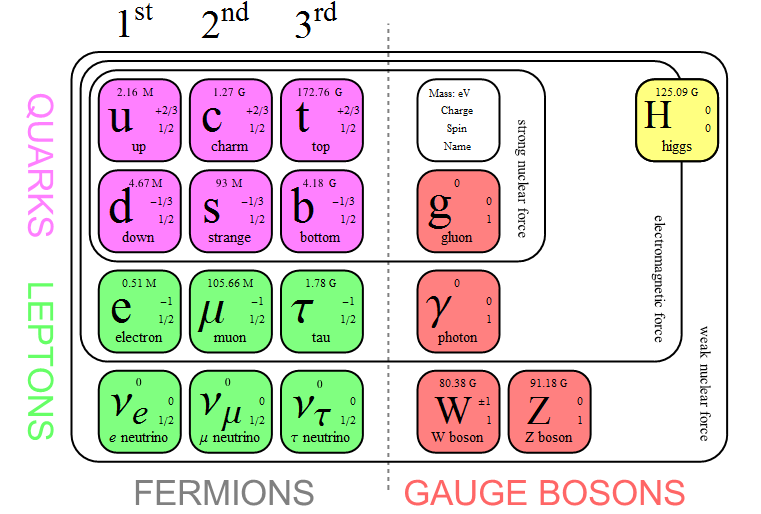
\includegraphics[scale=0.5]{figs/SM.png}
\caption{Schematic depiction of the SM. The masses of the in the SM massive particles are taken from \cite{PDG2020}. The electroweak force is divided into the electromagnetic force and the weak nuclear force. \cite{SMScheme}}
\label{fig:SM}
\end{figure}

The standard model of particle physics (SM) embodies our current understanding of the fundamental constituents of the universe and their interactions. It is a renormalizable quantum field theory constructed from a number of profound theoretical ideas to describe the experimental data observed. As often the case for theories in physics, the SM is guided by the principle of symmetry. Its local gauge symmetry group
\begin{equation*}
SU(3)_{C} \times SU(2)_{L} \times U(1)_{\gamma}
\end{equation*}
consists of the \textit{colour} symmetry group $SU(3)_{C}$ and the symmetry group of the \textit{hypercharge} $SU(2)_{W} \times U(1)_{\gamma}$. The hypercharge and the colour charge are related to the strong nuclear force and the electroweak force respectively. The subscripts $W$ and $\gamma$ indicate that electroweak force is the unification \cite{ModernPP} of the weak nuclear force and the electromagnetic force. $U(n)$ and $SU(n)$ are the unitary and special unitary groups of degree $n$ originating from the group theory structure of the SM \cite{GT}. Therefore, the SM contains two of the fundamental forces of nature. Gravity, which is the third fundamental force can be neglected at the particle level scales. \\
The particles in the SM are elementary particles that means they show no indication of substructure up to the current level of accuracy. All elementary particles can be categorized according to their spin statistics. Particles with half-integer spin obeying the Fermi-Dirac-statics are called \textit{fermions} while particles with integer spin are called \textit{bosons} which obey the Bose-Einstein-statistics \cite{FDStat}. Each particle has an associated antiparticle with the same mass and spin but opposite electrical charge, as well as lepton and baryon numbers. \\
Fermions are further subdivided into \textit{quarks} and \textit{leptons}. Quarks, contrary to leptons, can interact via the strong nuclear force. 
They come in 3 colours and 6 types called \textit{flavors} namely \textit{up}(u), \textit{down}(d), \textit{charm}(c), \textit{bottom}(b), and \textit{top}(t). Mathematically speaking quarks form 3 flavor doublets where the upper component has an electric charge of $Q=\frac{2}{3}$ and the lower an electric charge of $Q=-\frac{1}{3}$. From a physical point of view, this structure is reflected in three \textit{generation} of quarks. The $2^{\text{nd}}$ and $3^{\text{rd}}$ generation quarks have the same quantum number as the quarks from the $1^{\text{st}}$ generation but higher mass. Experimentally it was observed that quarks only exist in bound states of quark-antiquark pairs called \textit{mesons} or three quark or antiquark systems called \textit{baryons}, collectively called \textit{hadrons}. The standard model explains this behavior via \textit{colour confinement}, which states that coloured objects are always confined to colour singlet states and thus are colour neutral. In the case of quarks, the process of confinement is often referred to as \textit{hadronization}. \\
Similarly to quarks, the six leptons of the SM can be sorted into three generations each composed of a doublet. The lepton in the doublet that is electrically neutral and massless\footnote{Neutrinos are massless in the standard model. However, the observation of neutrino oscillations \cite{neutrinoOsci} indicate that they are massive.} is called a \textit{neutrino} ($\nu$). Their massive charge partners are called \textit{electrons} $e$, \textit{muons} $\mu$ and \textit{taus} $\tau$. \\
The forces in the standard model are mediated by \textit{gauge bosons}\footnote{The term ``gauge'' indicates that theories describing the forces are invariant under local gauge transformations \cite{GaugeInv}}. The gauge boson associated with the strong nuclear force is the \textit{gluon}. 
The gluon is a massless particle that carries colour charge. The electroweak force is mediated by three gauge bosons, two massive ones called W$^{\pm}$ and Z bosons, and one massless boson called \textit{photon}. The photon is the only gauge boson that does not carry its own charge and therefore can not self-interact. The strength of each interaction is modelled by energy depending coupling constants. \\
The Standard Model is summarized in Figure \ref{fig:SM}. The only SM particle not yet introduced the Higgs boson discovered in 2012 \cite{Higgs}. It can be interpreted as the excitation of the field predicted by the Higgs mechanism through which elementary particles acquire mass. \\
Even though the standard model is a remarkable achievement of modern science it's not the final answer. It has several shortcomings, for instance it neither provides a candidate for dark matter \cite{DM} nor explains the large matter-antimatter asymmetry in our universe\cite{MAM}.

\newpage  

\section{The Top Quark}
\label{sec:Top}

\begin{figure}[H]
\begin{subfigure}{.5\textwidth}
  \centering
  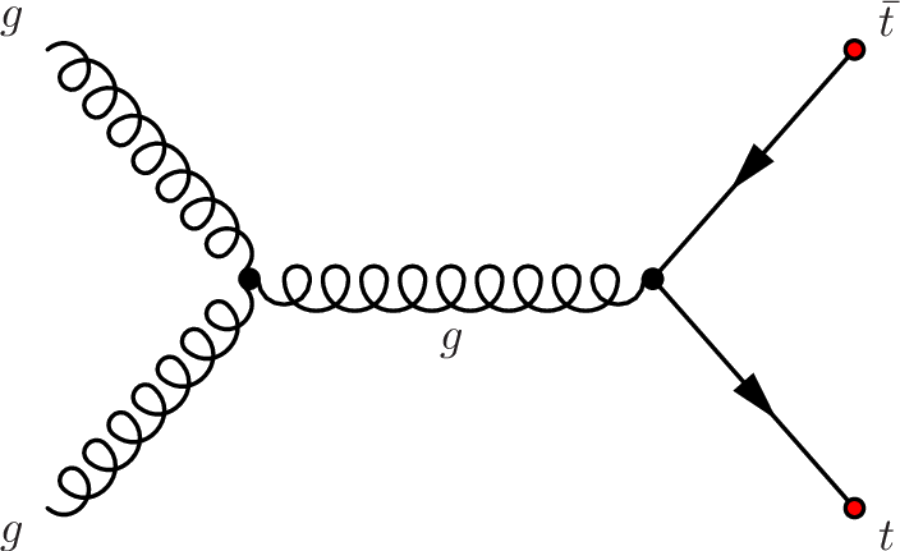
\includegraphics[width=.8\linewidth]{figs/TopPairProduction.png}
  \caption{Top pair production }
  \label{fig:PairProduction}
\end{subfigure}%
\begin{subfigure}{.5\textwidth}
  \centering
  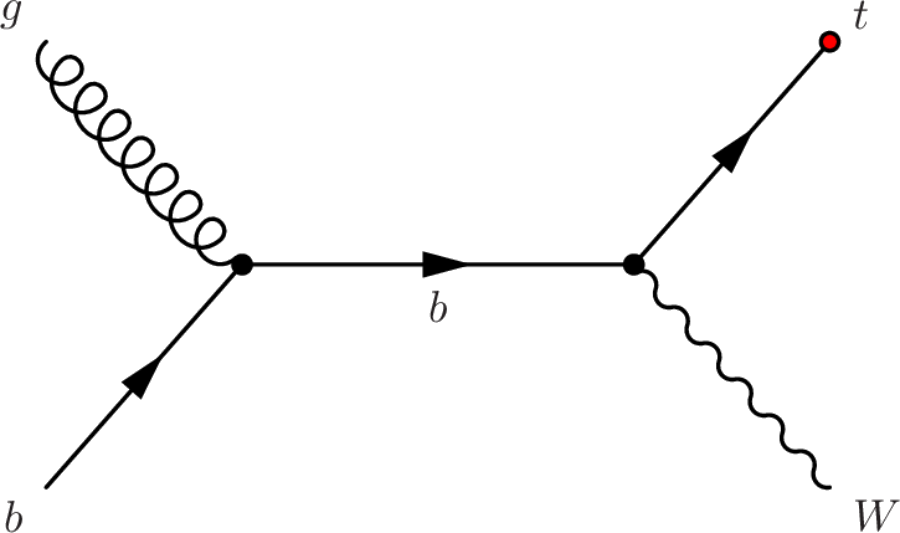
\includegraphics[width=.8\linewidth]{figs/SingleTopProduction.png}
  \caption{Single top production}
  \label{fig:SingleTopProduction}
\end{subfigure}
\caption{The two different categorizes of Top production}
\label{fig:TopProduction}
\end{figure}

The top quark has been first discovered in proton-antiproton collisions at the Fermilab Tevatron Collider in 1995 \cite{TopQuark}. It has a charge of $Q=\frac{2}{3}$ and was observed to be the most massive particle of the Standard Model. The Particle Data group reports a top mass of $m_{t} = 172.76 \pm \SI{0.30}{GeV}$ combing results measured at the Tevatron and the Large Hadron Collider \cite{PDG2020}. Therefore, it is $~40$ times heavier than the next-heaviest quark, the b quark. \\
Owing to its large mass, the lifetime of the top quark $\tau_{\text{t}} \approx 5 \cdot \SI[parse-numbers=false]{10^{-25}}{s}$ \cite{PDG2020} is very short. Consequently, it decays before it can hadronize, since typical time scales for interaction of the strong force are one order of magnitude higher. The decay to a W boson and a quark is governed by the CKM matrix \cite{ModernPP} of the electroweak interaction. Since decays in the same generation are enhanced, the matrix element $|V_{tb}|$ is much bigger than $|V_{ts}|$ and $|V_{tb}|$ resulting in an branching fraction of $BR = 0.90 \pm 0.04$ \cite{PDG2020}.  \\
The production modes of the top quark can be categorized into top-quark pair production and single top production. The processes in which the top is produced in pairs made up the main contribution of events in the discovery of the top quark. This is because processes producing single tops are governed by the electroweak interaction whereas top-antitop pairs are produced via the strong interaction, as can be seen in Figure \ref{fig:TopProduction}. Thus, the first evidence for single top processes was published considerably later in 2006 \cite{singlet}. An advantage of the single top production is that the CKM matrix element $|V_{\text{tb}}|^2$ can be measured directly \cite{CKMtb}.

\newpage

\section{Four-Top-Quark Production}
\label{sec:fourtops}
%The studies carried out in this thesis are related to the official four top-quark analysis of the ATLAS collaboration at $\sqrt{s} = 13$\,TeV [???]. 
The four-top-quark production ($\sigma_{t\bar{t}t\bar{t}}$) is one of the energetically highest processes accessible at the Large Hadron Collider (LHC). The center of mass energy $\sqrt{s}$ required to produce this process has to be at least 4 times the mass of the top quark. The most recent cross-section\footnote{The cross-section $\sigma$ and integrated Luminosity $\mathcal{L}$ will be introduced in Section \ref{sec:LHC}} calculation for proton-proton collisions predict $\sigma_{t\bar{t}t\bar{t}}=11.97^{+18\%}_{-21\%}$ at $\sqrt{s} = \SI{13}{TeV}$ \cite{ttttcross}. The cross-section calculation takes out of all possible production processes only those which are sub-leading in the strong or the electroweak coupling constant into account. Due to its small cross-section is $\sigma_{t\bar{t}t\bar{t}}$ are process which was not observed until now. The cross section of $\sigma_{t\bar{t}t\bar{t}}$ is enhanced in many beyond the Standard Model (BSM) sceneratios such as supersymmerty theories \cite{SuperS} or pair production of scaler gluons \cite{ScalarDing}. \\

\begin{figure}[H]
\begin{subfigure}{.5\textwidth}
  \centering
  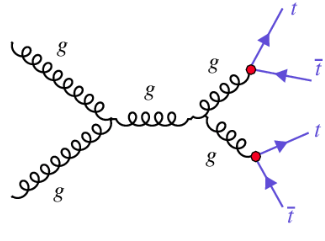
\includegraphics[width=.8\linewidth]{figs/4tproduction1.png}
  \caption{}
  \label{fig:4tproduction1}
\end{subfigure}%
\begin{subfigure}{.5\textwidth}
  \centering
  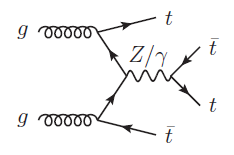
\includegraphics[width=.8\linewidth]{figs/4tproduction2.png}
  \caption{}
  \label{fig:4tproduction2}
\end{subfigure}
\caption{[INTNOTE] Two possible production processes of $t\bar{t}t\bar{t}$ in the SM.}
\label{fig:FourTopProduction}
\end{figure}

The Feynman diagrams of two $t\bar{t}t\bar{t}$ production processes are shown in Figure \ref{fig:FourTopProduction}. As mentioned in Section \ref{sec:Top}, the four top quarks will almost exclusively decay into a b quark and a W boson. The W boson can further decay either hadronically into two quarks or leptonically into a charged lepton and a neutrino, while the b quark will hadronize. The branching ratios for the possible leptonic `$\ell$' and hadronic `$h$' decay combinations are shown in Table \ref{tab:fourtopdecays} where the $\ell \ell hh$ channel is subdivided depending on the charges of the leptons. The $t\bar{t}t\bar{t}$ final state characteristics, therefore, are a high quark multiplicity and 4 b quarks. \\
The analyses of $t\bar{t}t\bar{t}$ carried out by the ATLAS and CMS collaborations are performed either in the one lepton opposite sign channel (1LOS) or in the same sign multilepton channel (SSML). The 1LOS channel considers final states that contain either one lepton or two leptons with opposite charges. The SSML considers final states that contain either two leptons with the same charge or at least 3 leptons. \\
CMS published results in the 1LOS channel and in the SSML channel using $\SI{13}{TeV}$ proton-proton collision data of $\mathcal{L} = \SI{36}{fb}^{-1}$. The quoted observed (expected) upper limits on the $t\bar{t}t\bar{t}$ cross-section are $\SI{48}{fb}$ ($\SI{52}{fb}$) \cite{cross1} and $\SI{41.7}{fb}$ ($\SI{20.8}{fb}$) \cite{cross2} . An updated preliminary result using $\mathcal{L} = \SI{137}{fb}^{-1}$ in the SSML leads to an observed (expected) upper limit of $\SI{22.5}{fb}$ ($\SI{8.5}{fb}$) \cite{cross3}. \\
The results published by the ATLAS collaboration combine the results of both channels and use proton-proton collision data at $\SI{13}{TeV}$ . The observed (expected) upper limit using $\mathcal{L} = \SI{36}{fb}^{-1}$ is $\SI{49}{fb}$ ($\SI{19}{fb}$) \cite{cross4}. The ATLAS analysis that uses the data with $\mathcal{L} = \SI{137}{fb}^{-1}$ is the fist search to claim evidence of four-top-quark production. The $t\bar{t}t\bar{t}$ production cross-section is measured to be $\SI[parse-numbers=false]{24^{+7}_{-6}}{fb}$ \cite{cross5}.

\begin{table}[H]
\centering
\begin{tabular}{|r|r|r|r|r|r|r|}
\toprule
& $hhhh$ & $\ell hhh$ & $\ell \ell hh$ OS & $\ell \ell hh$ SS & $\ell \ell \ell h$ & $\ell \ell \ell \ell$ \\
\midrule
$BR$ & 0.311 & 0.422 & 0.143 & 0.072 & 0.049 & 0.004 \\
\bottomrule
\end{tabular}
\caption{Branching fraction of the different decaying channel of $t\bar{t}t\bar{t}$ following from the decay of four $W$ bosons.}
\label{tab:fourtopdecays}
\end{table}


\section{Three-Top-Quark Production}
\label{sec:Theory3top}

A process that will become important in the analysis carried out in this thesis is the production of three top quarks ($t\bar{t}t$). The most dominant production processes and their branching fractions are shown in Table \ref{tab:BR3t}. All dominant production processes produce $t\bar{t}t$ in association with an additional particle. The most recent calculation of the three top quark cross-section for proton-proton collisions predict $\sigma_{t\bar{t}t} \approx \SI{2}{fb}$ at $\sqrt{s} = \SI{14}{TeV}$ \cite{3t}. \\
The final state of a $t\bar{t}t$ event has at least 3 b-quarks and a center of mass energy higher than 3 times the mass of the top quark. Depending on the decay of the W bosons and the particle produced in association with $t\bar{t}t$, different numbers of leptons, neutrinos, and quarks can be part of the final state composition.

\begin{table}[H]
\centering
\begin{tabular}{|r|r|}
\toprule
Process & branching frac. \\
\midrule
$pp \rightarrow t\bar{t}tW$ & 0.72 \\
$pp \rightarrow t\bar{t}tj$ & 0.19 \\
$pp \rightarrow t\bar{t}tb$ & 0.08 \\
\bottomrule
\end{tabular}
\caption{Dominant background processes and their branching fractions \cite{3t}}
\label{tab:BR3t}
\end{table}


%==============================================================================
\chapter{The Large Hadron Collider and the ATLAS Experiment}
\label{sec:ATLAS}
%==============================================================================

\section{The Large Hadron Collider}
\label{sec:LHC}
The Large Hadron Collider (LHC) is the world's largest particle accelerator. It's located at the European nuclear research center CERN at the french swiss border near Geneva. The construction of the collider started in 2000, along the $\SI{27}{km}$ long tunnel of its predecessor, the Large Electron-Positron Collider (LEP). Over ten thousand scientists from more than 100 countries contributed to its construction. The LHC was designed to collide protons with a center of mass energy of $\sqrt{s}= \SI{14}{TeV}$, to push the limits of our understanding of particle physics, conditions similar to those of the very early universe. \\
During Run 1 of the LHC in the years 2010 to 2012 a center of mass energy of $\sqrt{s}= 7-\SI{8}{TeV}$ was reached. The most famous discovery made during this time period is the observation of the last missing ingredient of the SM, the Higgs boson in 2012 by the ATLAS and CMS collaborations \cite{Higgs}. After two years of construction work, Run 2 started in 2015 and ended in 2018. During Run 2, properties of the Higgs boson such as its Yukawa coupling to the heaviest, third-generation quarks and leptons were investigated. Moreover, many precision measurements of SM parameters were executed to search for physics beyond the Standard Model (BSM). \\


\begin{figure}[H]
\centering
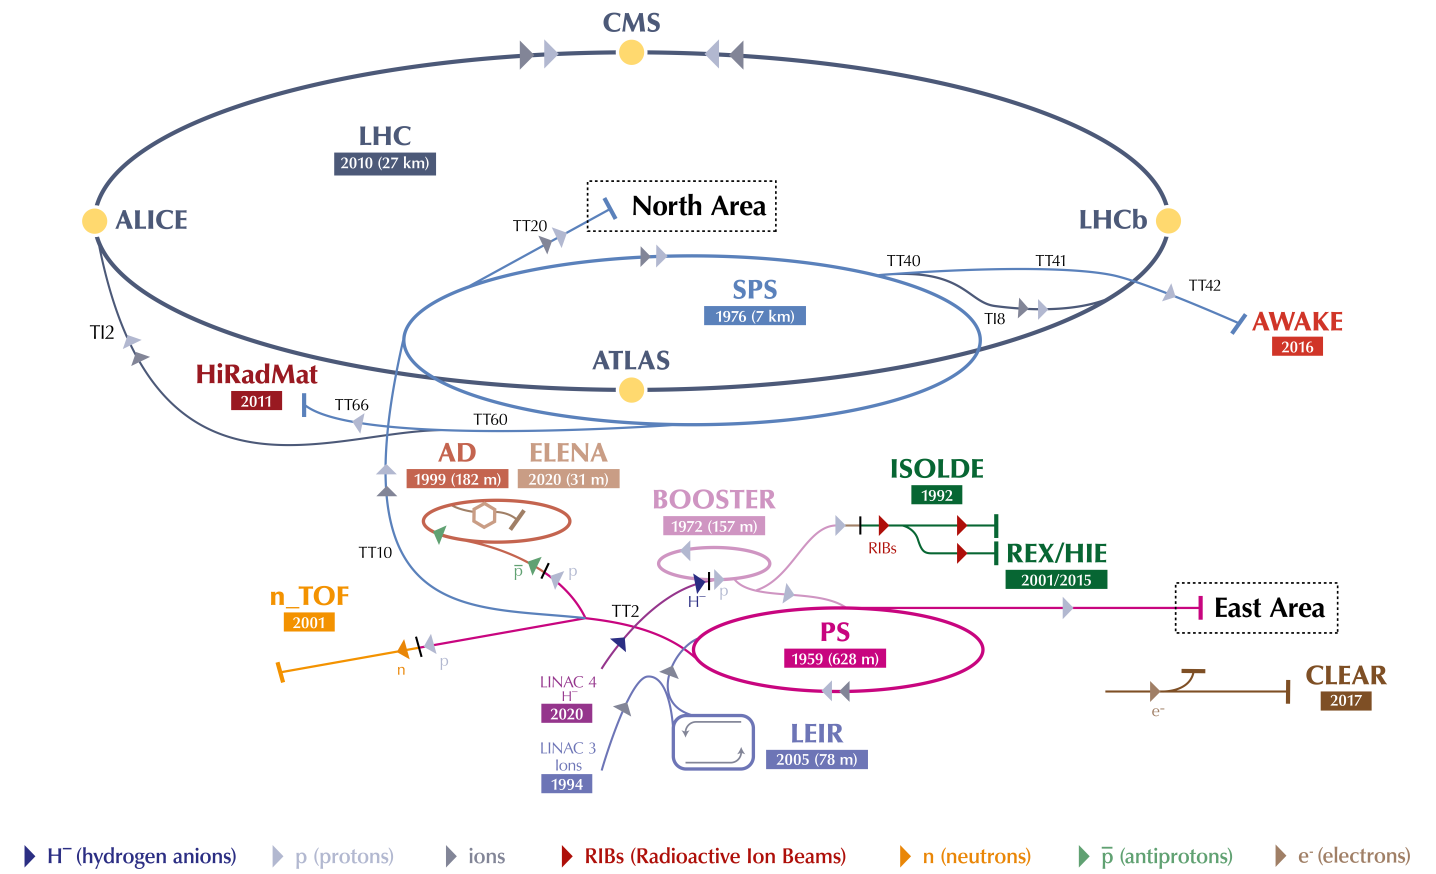
\includegraphics[scale=0.215]{Cern}
\caption{The accelerator complex of CERN including the LHC. The accelerator chain for the protons is shown as well as the four major experiments.\cite{CernAcc}}
\label{fig:Cern}
\end{figure}

\newpage

\paragraph{Proton Acceleration} \mbox{} \\

The protons that will be accelerated to the TeV energies originate from hydrogen atoms in a bottle. After their ionization, the protons are pre-accelerated to $\SI{450}{GeV}$, and squeezed into \textit{bunches}. The three pre-accelerators Linac 2, PSB, and SPS are shown in Figure \ref{fig:Cern}. The bunch trains of protons entering the LHC are separated by \SI{25}{ns} and containing $1.15\cdot 10^{11}$ protons. They are further accelerated by electrical fields and focused via magnetic fields of $\SI{3}{T}$ provided by superconducting dipole and quadrupole magnets. The LHC itself consists of two parallel vacuum rings in which protons travel in opposite directions. Once the protons have reached the desirable energy, they collide at 4 interaction points. At each point, one detector is located, namely ATLAS, CMS, ALICE, and LHCb. The ATLAS and CMS detectors are general-purpose detectors looking for particle properties and BSM physics. The LHCb experiment is the only fixed target experiment at CERN and is focused on heavy flavour physics. The fourth experiment ALICE studies heavy-ion physics such as quark-gluon plasma. \\

\paragraph{Luminosity and Pile-up} \mbox{} \\

Rare high energetic processes such as $t\bar{t}t\bar{t}$ can only be observed if the center of mass energy is high and enough particle collisions take place. If a collider produces the required number of events is quantified by its Luminosity $L$. It's defined by the formula
\begin{equation}
\label{eq:Lumi}
L = \frac{1}{\sigma} \frac{dN}{dt} \cdot \epsilon \,  \,; \, \,\,\,\,\,\,\,\,\, [L] = \text{m}^{-2}\text{s}^{-1}=\text{fb}^{-1}
\end{equation}
where $\sigma$ is the cross-section, giving the number of events that are recorded per unit area and $\epsilon$ the detector efficiency defined as the fraction of events which are measured in the detector relative to the number of events produced. The design Luminosity of the LHC is $L = \SI[parse-numbers=false]{10^{34}}{m}^{-2}\text{s}^{-1}$, however, it has been surpassed during Run 2. Of practical importance is the integrated Luminosity $\mathcal{L}$
\begin{equation}
\mathcal{L} = \int L dt
\end{equation}
since the Luminosity add up with time and can vary depending on collider conditions. One drawback of high Luminosities is that multiple interactions at the same bunch crossing take place. However, only the interaction with the highest energy is of interested called the \textit{hard scattering event}. All events originating from other interactions are called \textit{pile-up} $<\mu>$. In practise its a challenging task to identify and remove particles coming from pile-up.

\section{The ATLAS Experiment} 
\label{ATLAS}
The ATLAS detector is the largest general-purpose detector at the Large Hadron Collider. Its main purpose is to search for new undiscovered particles and probe the SM by taking advantage of the high energetic protons available at the LHC. This section introduces the coordinate system and the structure of the ATLAS experiment as well as the particle reconstruction. \\


\paragraph{The ATLAS Coordinate System} \mbox{} \\
The coordinate system of the ATLAS experiment is right-handed with its origin at the interaction point. The z-axis is orientated in the direction of the beam pipe while the x-axis points to the center of the LHC, the points upwards. Cylindrical coordinates (z,$\Phi$,$\theta$) are a natural choice where $\Phi$ is the azimuthal angle around the beam pipe and $\theta$ the polar angle. A commonly used variation of $\theta$ is the pseudorapidity $\eta$
\begin{equation}
\label{eq:eta}
\eta = - \ln[\tan(\frac{\theta}{2})]
\end{equation}
where $\eta =0$ corresponds to the center of the detector and $\eta \rightarrow 0$ points to the beam axis. The advantage of this definition is that the outgoing particle rate per unit $\eta$ is on average constant. \\
The proton-proton collisions at the interaction point break up the inner structure of the protons resulting in new particles and particle \textit{jets}.\textit{Jets} in the context of particle physics refers to narrow cones of hadrons and other particles produced during the hadronization of quarks or gluons. The particles originating from the proton-proton have to have a total transverse momentum $p_{\text{T}}=p_{\text{x}}+p_{\text{y}}$ of zero since the partons of the initial protons, quarks and gluons, have negligible momenta in the transverse plane due to their high boost in the z-direction.

\paragraph{Inner Detector} \mbox{} \\

\begin{figure}[H]
\centering
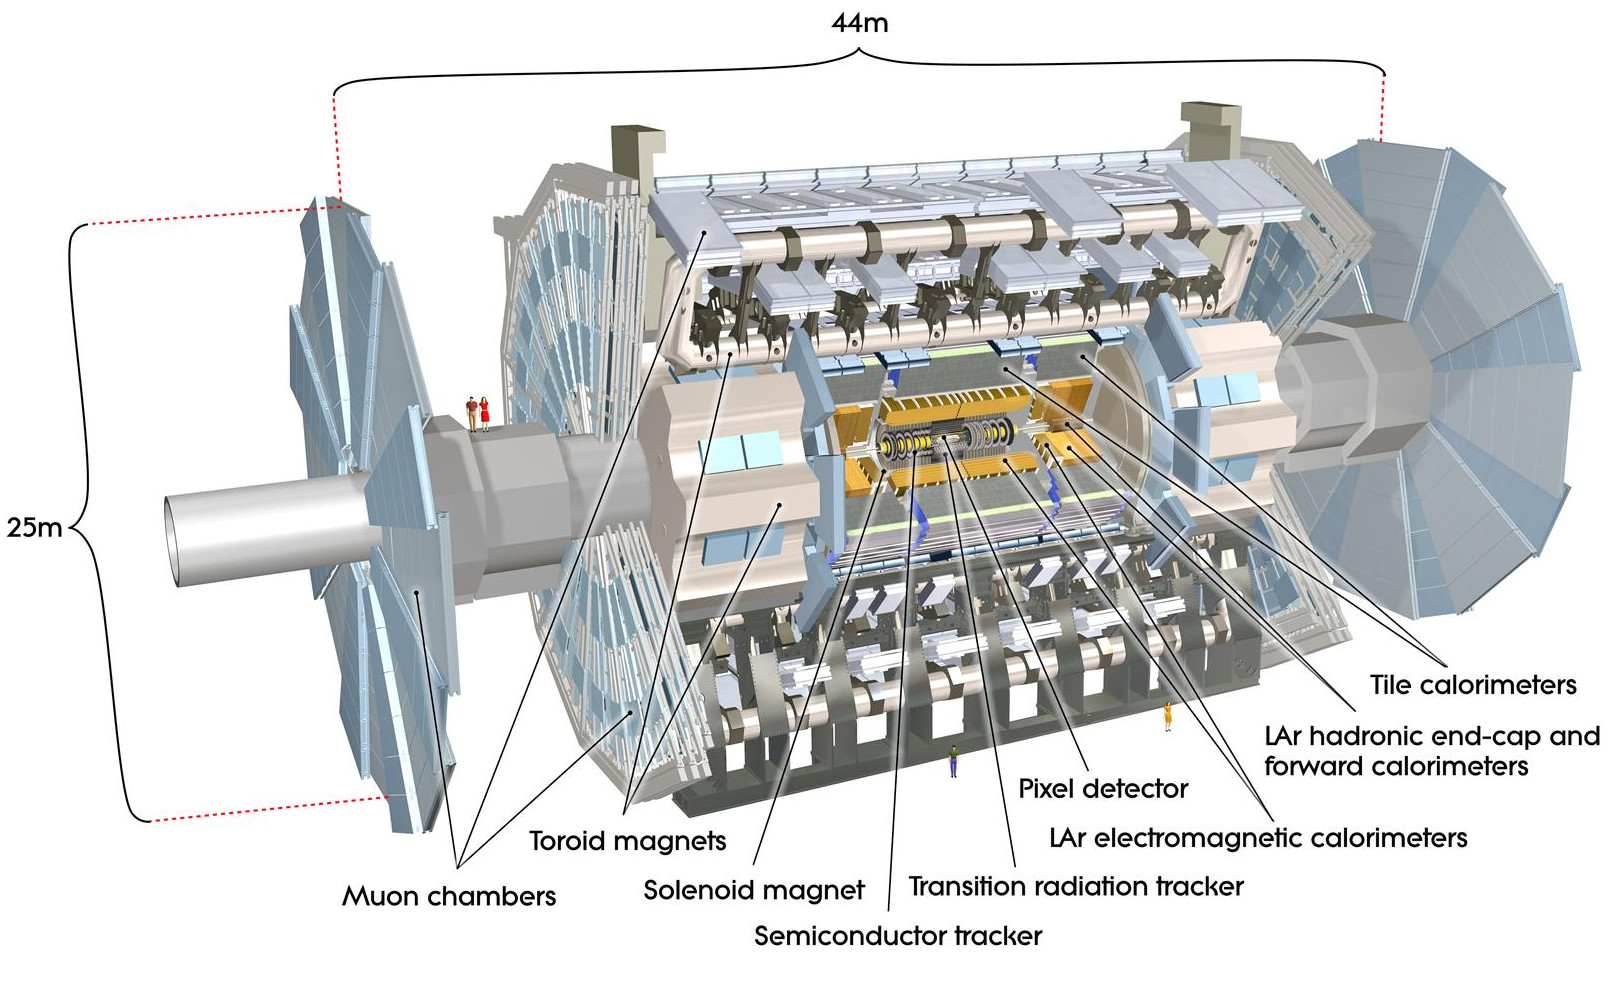
\includegraphics[scale=0.2]{ATLAS}
\caption{Illustration of the ATLAS detector and its sub-units.\cite{ATLASP}}
\label{fig:ATLAS}
\end{figure}

The track, momentum, and energy of particles are measured in cylindrically arranged detector layers surrounding the beam pipe, as shown in Figure \ref{fig:ATLAS}. The layer closest to the interaction point is called the inner detector and covers a pseudorapidity range of $|\eta| < 2.5$. It's composed of several highly granulated tracking detectors such as silicon pixel detectors and transition radiation detectors for particle identification. The super-conducting solenoid magnets provide a $\SI{2}{T}$ magnetic field in which the trajectory of charged particles are bent. The radius of this curve together with the tracking information provided by the inner detector can then be used to measure the particles momenta. 

\paragraph{Calorimeters} \mbox{} \\
The calorimeter of the ATLAS experiment enables the measurement of particle energies through interactions with the detector material. Particles entering the calorimeters initiate showers until they are stopped. The length of these showers is proportional to the energy deposited by the particle. The ATLAS calorimeter system consists of two different calorimeters an electromagnetic calorimeter (ECAL) and a hadronic calorimeter (HCAL). Showers initiated in the ECAL are governed by the electroweak interaction, therefore, the chosen material is a gas (liquid  Argon). On the other hand, the HCAL contains scintillator crystals adjusted for the hadronic showering. The pseudorapidities covered by the ECAL are $1.36 < |\eta| < 3.2$ and $1.7 < |\eta| < 3.2$ for the HCAL, excluding the \textit{crack region} $1.3 < |\eta| < 1.52$ between the barrel and the end cap.

\paragraph{Muon Spectrometer} \mbox{} \\
The outermost layer of the ATLAS detector is the muon spectrometer. Muons are Minimum Ionizing Particles (MIPs) for a range for $\mathcal{O}(100)$ MeV up to the TeV scale. Therefore, they only deposit a small fraction of their energy in the calorimeters. To identify and measure the properties of muons, gaseous detectors in a magnetic field are used. A muon passing through such a detector ionizes the gas. The ions and electrons drift in an electrical field and induce a signal. The muon spectrometer of the LHC has a magnetic field of $\SI{0.5}{T}$ to $\SI{1}{T}$ and covers a range of $|\eta| < 2.7$.


\paragraph{Object reconstruction} \mbox{} \\

\begin{figure}[H]
\centering
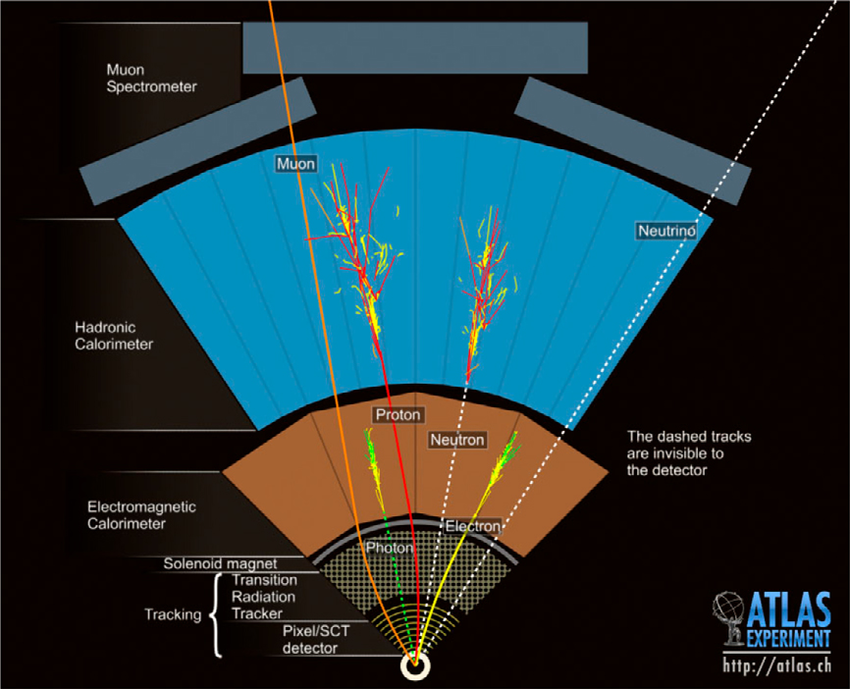
\includegraphics[scale=0.8]{ATLAS_interactions}
\caption{Interaction of different types of particles with different segments of the ATLAS detector.\cite{ATLASint}}
\label{fig:Interaction}
\end{figure}

The detector signals of the different particles (cf. Figure \ref{fig:Interaction}) have to be converted into physics objects. Since many particles such as the top quark or W and Z bosons decay before reaching the detector they have to be identified via their long-living decay products. A process referred to as reconstruction. Notably, the reconstruction of most physics objects is performed independently. The overlap removal is then performed dependent on the goal of the analysis carried out. \\
While leptons, photons, and jets can be identified by their interaction with the different detector components, neutrinos do not interact with any part of the detector. They have to be identified via the conservation of transverse momentum. The deviation of the total $p_{\text{T}}$ sum from zero is an indication for the presence of neutrinos or other exclusively weakly interacting BSM particles. The missing transverse momentum can be defined as
\begin{equation}
\label{eq:Etmis} 
E_{\text{T}}^{\text{miss}} = - \sum_{i \in {\text{final state particles}}} p_{\text{T},i}
\end{equation}
Of special interest for the reconstruction of top quarks, and thus the $t\bar{t}t\bar{t}$ process, are the b-jets originating from the hadronization of b quarks. The B hadrons contained in the b-jets have a long lifetime and usually decay within the tracking detectors. Therefore, a secondary decay vertex can be identified. To improve the efficiency of b-tagging further, kinematic properties such as the mass and the fragmentation of B Hadrons are utilized. 

%==============================================================================
\chapter{Datasets and Event Selection}
\label{sec:Samples}
%==============================================================================
This chapter introduces the datasets uses for the Neural Network studies carried out in the following chapters. An overview of the steps taken to simulate the different background and signal datasets is given as well as a short introduction of event weights. The chapter is then concluded by the description of the event selection and the definition of the signal region.

\section{Simulated Datasets}
\label{sec:Simulation}
The data used in this thesis does not come from real proton-proton collisions measured in the ATLAS detector but rather is simulated data. These simulations are essential to accurately estimate the underlying background and for optimal signal selection. The ATLAS simulation chain \cite{ATLASsim} can be divided into three steps: generation of the event and immediate hadronization and decay of the produced particles, simulation of the particle interaction with the detector such as parton showering,  and digitization of the detector responses into voltages and currents. The event generation can proceed at different levels of precision. A leading-order (LO) event generation only takes those production processes into account that have the smallest power of the coupling constant among all possible contributing processes. On the other hand, a next-to-leading-order (NLO) calculation additionally considers production processes which are sub-leading in the coupling constant power.  \\
The datasets used for the signal and all backgrounds are simulated to match the full Run 2 dataset. It consists of three sub-campaigns MC16a corresponding to the data taking conditions in the years 2015 and 2016, MC16d for the year 2017, and MC16e for the year 2018. The $t\bar{t}t\bar{t}$ events are simulated using {\scshape MadGraph5\_Amc@NLO} \cite{MadGraph} at NLO precision. The top quarks are decayed at LO using {\scshape MadSPIN} whereas the parton showers and hadronization processes are modeled by {\scshape Pythia8}\cite{PYTHIA}. In addition to the first NLO $t\bar{t}t\bar{t}$ dataset, a second signal dataset produced at LO precision is available. \\
The background datasets are summarized in table \ref{tab:generatros} together with the used event generators and parton shower simulation programs. All backgrounds expect $t\bar{t}$+Diboson and $V$+jets\footnote{$V$ corresponds to either a W or a Z boson} are produced at NLO precision. $t\bar{t}$+Diboson was generated at LO but scaled the NLO cross-section. $V$+jets is simulated at NLO for up to two jets and at LO for up to four jets. The dataset referred to as ``others'' mainly contains $t\bar{t}t$ events but also $VH$ and $VVV$ events. More details about the datasets can be found in the official ATLAS four-top-quark analysis \cite{cross5}. The final simulation step of the ATLAS detector responses to the different final state particles is modeled by {\scshape AltFast} \uproman{2} \cite{AltFast}. \\
An additional dataset containing $t\bar{t}t\bar{t}$ and $t\bar{t}t$ events was simulated (MC16e only) for reconstruction studies and will not be used as an additional background in the $t\bar{t}t\bar{t}$ analysis. Similar to all other samples it contains information about reconstructed objects. Additionally, information not available at reconstruction level called \textit{truth information} is available for this dataset. An example for truth information would be the information if a W boson decays hadronically or leptonically. The $t\bar{t}t$ events are generated by {\scshape MadGraph5\_Amc@NLO} while the parton showering is simulated using {\scshape PYTHIA8}. 

\begin{table}[H]
\centering
\begin{tabular}{|r|r|r|}
\toprule
Dataset & Event generator & parton showering \\
\midrule
\midrule
$t\bar{t}t\bar{t}$ & \scshape MadGraph5\_Amc@NLO & \scshape PYTHIA8 \\
$t\bar{t}W$ & \scshape Sherpa \cite{Sherpa} & \scshape Sherpa \\
$t\bar{t}WW$ & \scshape MadGraph5\_Amc@NLO & \scshape PYTHIA8 \\
$t\bar{t}Z$ & \scshape MadGraph5\_Amc@NLO & \scshape PYTHIA8 \\
$t\bar{t}H$ & \scshape PowHegBox \cite{PowHeg} & \scshape PYTHIA8 \\
$t\bar{t}$ & \scshape PowHegBox & \scshape PYTHIA8 \\
$t(\bar{t})X$ & \scshape PowHegBox & \scshape PYTHIA8 \\
$V$+jets & \scshape Sherpa & \scshape Sherpa \\
$VV$ & \scshape Sherpa & \scshape Sherpa \\
others & MadGraph5\_Amc@NLO & \scshape PYTHIA8 \\
$t\bar{t}t$ & \scshape MadGraph5\_Amc@NLO & \scshape PYTHIA8 \\
\bottomrule
\end{tabular}
\caption{Summary of the event generator and parton showering programs used for the different datasets.}
\label{tab:generatros}
\end{table}

\paragraph{Event Weights} \mbox{} \\

The datasets described above contain combined $\sim 2700000$ events that pass the preselection which will be introduced in the next section. The $t\bar{t}W$ datasets contains $\sim 400000$ events while the NLO $t\bar{t}t\bar{t}$ dataset contains $\sim 500000$ events. However, the cross-section of the $t\bar{t}W$ at 13TeV is an order of magnitude larger than the cross section of four-top-quark events and even after applying the preselection the ratio is still approximately 20 (c.f. Figure \ref{fig:HT_preselection}). The number of generated data events $N_{\text{gen}}$ for each process can be scaled to the number of events measured in the detector and passing all preselections $N_{\text{pass}}$ by applying Luminosity weights $w _{\text{Lumi}}$ defined by
\begin{equation}
\label{eq:weights}
w _{\text{Lumi}} = \frac{N_{\text{exp}}}{N_{\text{pass}}} = \frac{\sigma \cdot L}{N_{\text{gen}}}
\end{equation}
which directly follow from Equation \ref{eq:Lumi} by expressing $\epsilon$ as $\frac{N_{\text{pass}}}{N_{\text{gen}}}$. Moreover, different event by event weights have to be applied to account for different beam and detector configurations such as pile up, lepton scaling factor, jet vertex tagger, and b-tagging scaling factor weights. A special weight is the generator weight \cite{PDG2020}, originating from the evaluation of the phase space integral during the generation of the events. For next to leading order event generation this weight can become negative due to the calculation contribution of loop amplitudes \cite{nWeights} which often can be problematic for machine learning methods. The effective number of observable events after applying the weight sum will be referred to as event \textit{Yield}.

\section{Object and Event Selection}
\label{sec:EventSelection}

The signal and background datasets contain four different reconstructed objects electrons, muons, jets, b-jets and $E_{\text{T}}^{miss}$. An overlap removal procedure depending on the distance between two objects is applied to ensure that calorimeter clusters and particle tracks are not signed twice to different objects. \\
The event preselection will be defined in the following. Events passing the preselection have to have fired a single-lepton or dilepton trigger. The $p_{\text{T}}$ threshold of these triggers vary depending on the fulfilled isolation requirements of the leptons and the data-taking period. Only those events which have at least one vertex reconstructed from at least two inner detector tracks with transverse momenta of $p_{\text{T}}>\SI{0.4}{GeV}$ are considered. The kinematic preselection requirements for leptons and jets are summarized in Table \ref{tab:requirements}. Additionally, the electron charge identification selector (ECIDS) \cite{ECIDS} is applied for final states with two electron or an electron and a muon. The ECIDS suppress the charge misidentification background significantly. Jets are reconstructed using the anti-k$_{t}$ algorithm \cite{Akt} (R = 0.4). To reduce pile-up, jets are furthermore required to have a transverse momentum of $p_{\text{T}}$ and $|\eta| < 2.4$. B-jets are identified using a multivariate algorithm called MV2c10 \cite{MV2c10} , where c10 refers to the fact that 10\% of the background dataset are c-jets. The pseudo-continuous working points provided are 80\%, 77\%, 70\%, and 60\% b-tagging efficiency. The working point selected for this analysis is 77\% b-tagging efficiency.
 
\begin{table}[H]
\centering
\begin{tabular}{|r|r|r|}
\toprule
Particle type & $p_{\text{T}}$ & $|\eta|$ \\
\midrule
\midrule
Electrons & $> \SI{28}{GeV}$ & $<2.47$ \\
Muons & $> \SI{28}{GeV}$ & $<2.5$ \\
Jets & $> \SI{25}{GeV}$ & $<2.5$ \\
B-jets & $> \SI{28}{GeV}$ & $<2.5$ \\
\bottomrule
\end{tabular}
\caption{Transverse momentum and pseudorapidity preselections for the different particles, the crack region is excluded.}
\label{tab:requirements}
\end{table}


\paragraph{Signal Region} \mbox{} \\

Events entering the signal region come from the Same Sign Multi-Lepton channel SSML where two same-sign leptons or at least three leptons are required. The branching fraction of this channel is $BR = 0.12$ (cf. Table \ref{tab:fourtopdecays}) where the biggest contribution originates from the same signed lepton events $BR = 0.07$. The definition of the signal region is then completed by requiring at least 6 jets among which are at least two b-tagged as well as a scalar sum of all lepton and jet $p_{\text{T}}$'s $H_{\text{T}}$ high than $\SI{500}{GeV}$.   \\
Figure \ref{fig:HTSR} shows the $H_{\text{T}}$ distributions before the definition of the signal region is applied (a) and after (b). As can be seen, the amount of background events is significantly decreased in the signal region. To quantify this observation the \textit{signal efficiency} $s$ is defined as
\begin{equation}
\label{eq:sigeff}
s = \frac{Y_s}{\sqrt{Y_s + Y_b}}
\end{equation}
where $Y_s$ and $Y_b$ are the signal and background Yield. The calculated values for the signal efficiency after allying the requirements of the signal region and before are 0.8 and 1.8. The total number of events available for training Neural Networks, introduced in Chapter \ref{sec:Deep_learning}, decreases to $\sim 700000$ events. The number of events fulfilling the preselection and in of the signal region are summarized in Table \ref{tab:prevssr} in the Appendix. The dominant backgrounds in the signal region are $t\bar{t}W$, $t\bar{t}Z$ and $t\bar{t}H$. The backgrounds coming from $t\bar{t}X$ are split depending on the instrumental effects and physics processes that lead to a final state similar to that of $t\bar{t}t\bar{t}$ event:
\begin{enumerate}[leftmargin=2cm]
\item[QmisID:] events with one lepton having its charge mis-identified
\item[CO:] events with one lepton coming from photon material conversion
\item[HF:] events with one lepton coming from heavy-flavour meson decay
\item[light:] events with one lepton coming from light-meson decay or events with one wrongly identified jet as a lepton
\item[other:] events falling into none of the above categories
\end{enumerate}
Minor backgrounds are diboson production $VV$, associated production of bosons with jets $V$+jets, single top $t(\bar{t})X$ and $t\bar{t}WW$ as well as the previously introduced datasets of ``others''.


\begin{figure}[H]
\begin{subfigure}{\textwidth}
  \centering
  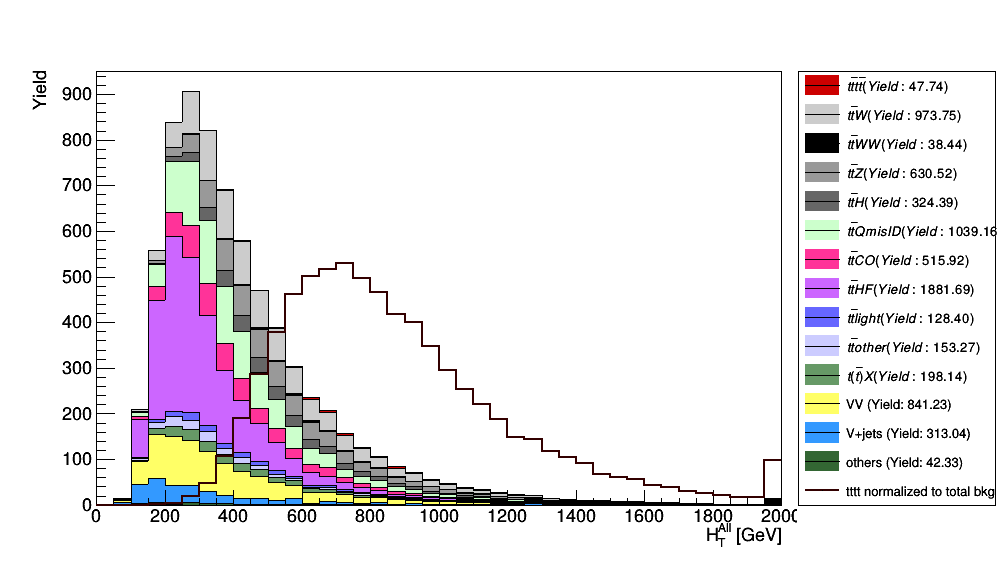
\includegraphics[width=.95\linewidth]{figs/HT_presection.png}
  \caption{Preselection}
  \label{fig:HT_preselection}
\end{subfigure} \\
\begin{subfigure}{\textwidth}
  \centering
  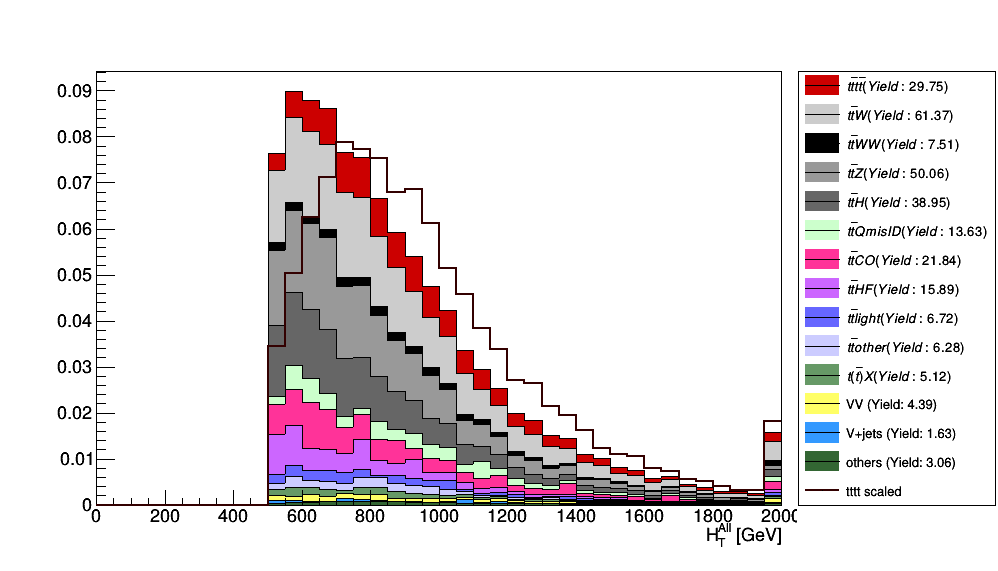
\includegraphics[width=.95\linewidth]{figs/HT_sr.png}
  \caption{Signal Region}
  \label{fig:HT_sr}
\end{subfigure}
\caption{Sum of the transverse momentum of all leptons and jets ($H_{\text{T}}$) after applying the preselection (a) and in the signal region (b). The dark red line shows the signal scaled to the total background yield. The last bin contains additionally all events with $H_{\text{T}} > 2000$}
\label{fig:HTSR}
\end{figure}
%==============================================================================
\chapter{Introduction to Deep Learning}
\label{sec:Deep_learning}
%==============================================================================
Deep learning, as a sub-field of machine learning, is concerned with the study of algorithms that have the ability to learn through experience. The experience is typically gained by presenting the algorithm with data examples from which it learns a set of rules. In the particular case of deep learning, the models considered are Deep Neural Networks (DNNs). \\
In this chapter, Artificial Neural Networks (ANNs) are introduced first before turning to the more advanced DNNs. Two different types of DNNs, namely Feedforward Neural Networks (FNNs) and Recurrent Neural Networks (RNNs) and their training algorithms will be discussed. Furthermore, different types of activation functions, weight initializations, and optimization algorithms are reviewed. Special emphasis is put on the application to \textit{supervised classification tasks} which is the kind of problem at hand in the latter chapters of this thesis. 

\section{Artificial Neural Networks}
\label{sec:ANNs}
\begin{figure}[H]
\centering
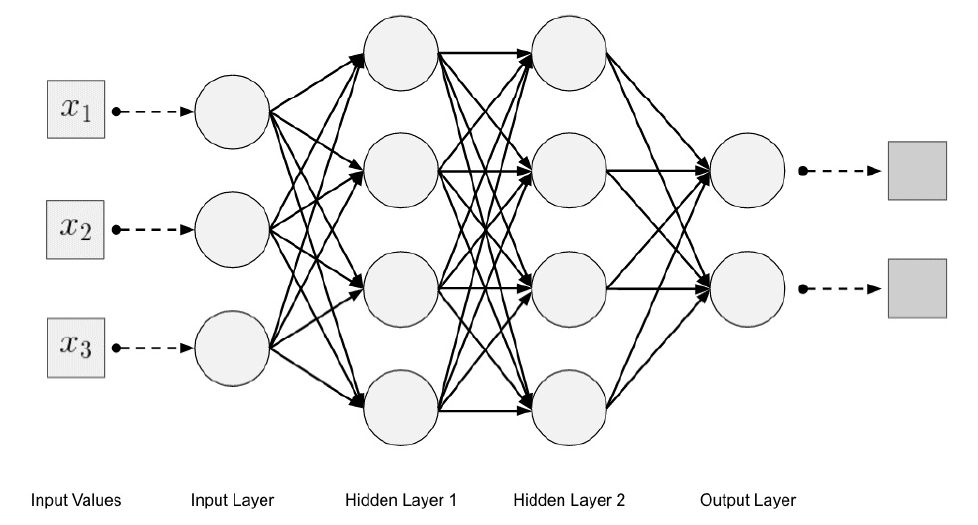
\includegraphics[scale=0.37]{figs/NeuralNetwork.png}
\caption{Schematic structure of a deep neural network with fully connected layers. The input values of the given task $x_i$ are fed into the neurons (depicted as circles) of the input layer and processed in the hidden layers. The weights which connect neurons located at different layers are represented by a solid arrow. In the output layer, all information is combined and predictions (depicted as dark squares) about the classes are made. (Figure taken from \cite{patterson2017deep})}
\label{fig:NeuralNetwork}
\end{figure}
As it is often the case for inventions in science and technology, the idea of ANNs is inspired from nature, more precisely by the human brain. The two key principles involved in the decision-making process of human brains are recognizing patterns and inductive thinking \cite{logan2018thinking}. These, for any machine learning model, highly desirable attributes, are modeled by imitating the structure of the human brain in an ANN. \\
The basic building blocks of the brain, neurons, process and transmit information via electric and chemical signals. The input signals received by a neuron is summarized to a net input $z$. This net input is then compared to an internal threshold. The output of the neuron is 1 if the threshold is passed and 0 otherwise. Since the summarization process of all the input signals to the net input is still part of on going research in the field \cite{bioNeuron}, the net input $z$ for artificial neuron is simply defined to be
\begin{equation}
z=b + \sum_i x_i w_i
\end{equation}
where $w_i$ are weights representing the assigned importance of the different features $x_i$, b is the bias term which is the the artificial equivalent of the threshold in a biological neuron. Additionally, an arbitrary \textit{activation function} $\Phi(z)$ is applied to the net input corresponding to the unknown degrees of freedom in the decision-making process and determining the final output of the artificial neuron. \\
The neurons in an ANN are structured as layers, shown in Figure \ref{fig:NeuralNetwork}. The first layer is called the \textit{input layer}, containing all the input features. In practice, these input features are physical variables such as kinematic quantities of the final state particles. The layers following the input layer are called \textit{hidden layers}. If an ANN has more than one hidden layer it is considered a DNN and thus, by definition a deep learning model. The different layers are connected to their successors via weight vectors $\vec{w}$. Depending on the magnitude of the weights a neuron can focus on a combination of features provided by the neurons in the previous layer. The model complexity and flexibility, therefore, increases with the number of neurons $n$ and layers $\ell$ it contains. In the case of fully connected layers, i.e. every neuron in a given layer is connected to all neurons in the previous layer, the number of free parameters (weights and bias) can be calculated according to
\begin{equation}
\sum_{\ell=1}^{L} n^{\ell-1} n^{\ell} + n{^\ell}
\label{eq:NumPara}
\end{equation}
where $L$ is number of layers in the Neural Network. The last layer is called the \textit{output layer} where all information is compressed and predictions are made. In this thesis, the prediction made is the affiliation of an event to a signal or background process. In terms of machine learning language, such a problem is called a \textit{supervised classification task} where the supervision is given by the correct assignment known from the simulation. To get the classification right, an ANN has to learn which combination of features ultimately results in the best separation between the different classes. This process is often referred to as \textit{training} and is discussed in the next section.

\section{Training of Feed-Forward Neural Networks}
\label{sec:training}
There are several different types of Neural Network, each adjusted and optimized for their specific field of application. However, they all share a similar, gradient-based training procedure that can be best understood considering Feed-Forward Neural Networks\footnote{The name originates from the fact that, in an FNN information is always passed forward. Different types of ANNs also involve a cyclic flow of information within one neuron (see section \ref{sec:RNN})} (FNNs). \\
The first step of any gradient-based method is the \textit{forward pass}. The forward pass involves the evaluation of the net input and the activation function for each neuron successively. The neuron output values $a=\Phi(z)$ are preserved for the necessary gradient calculations later in the training. The forward pass is applied for each event individually such that the predictions made in the output layer results in a prediction distribution $p$. This distribution is used to evaluate the current performance of the neural network based on a \textit{loss function}.

\newpage
\paragraph{Loss function} \mbox{} \\
The loss function $L(\theta)$ is a measure of how close $p$ is to the true distribution $y$, and depends on the weight tensor $\theta$ which includes all trainable parameters\footnote{The bias term can be reinterpreted as the weight $w_0 = -1$ of the weight tensor \cite{NNTheory}}. The training of an FNN is said to have converged if the trainable parameters are adjusted such that the loss function is at its global minimum i.e. for all events the predicted probability is as close as possible to the true class. \\
A  commonly chosen loss function for classification task is the cross-entropy loss \cite{Crossentro} defined for $K=2$ classes and m events as
\begin{equation}
L(\theta) = - \frac{1}{m} \sum^{m}_{i=1} \sum^{K}_{j=1} y^{(i)}_{j} \cdot \ln(p^{(i)}_{j}) = - \frac{1}{m} \sum^{m}_{i=1} [y^{(i)} \ln(p^{(i)}) + (1-y^{(i)})\ln(1-p^{(i)})]
\label{eq:crossent}
\end{equation}
where $p^{(i)}_{j}$ is the predicted probability that the $i^{th}$ event belongs to class $j$ and $y^{(i)}_{j}$ is either 1 if the true class of the event is j or 0 otherwise. It can be derived from the Kullback-Leibler Divergence \cite{Kulldiv} and thus interpreted as the likelihood that $p$ could have been generated by $y$. Selecting the cross-entropy loss avoids small values in the gradient calculations which is key for fast convergence of the training algorithm discussed in the next sub-section.

\paragraph{Backpropagation algorithm} \mbox{} \\
The most widely used training algorithm is called the Backpropagation algorithm \cite{backpro}. In addition to the first forward pass, a second backward pass is performed. In the backward pass, weight updates for each weight in the ANN are calculated based on the neuron outputs obtained in the forward pass. The exact execution of the weight updates depends on the optimization algorithm chosen. Nevertheless, most optimization algorithms are variations of the simple gradient descent method. Gradient descent calculates the partial derivatives of the loss function for each weight, exploiting the chain rule. In the case of the cross-entropy loss for a single event, the derivative with respect to the weight between the $j^{th}$ neuron in layer $\ell$ and the $k^{th}$ neuron in previous layer $\ell-1$ is given by
\begin{equation}
\label{eq:part_deriv}
\frac{\partial L}{\partial w^{\ell}_{jk}} =  \frac{1}{n} \sum_{k=0}^n x^{\ell-1}_{k} (\phi(z^{\ell}_{j})-y_{j}) 
\end{equation} 
where the predicted distribution $p$ in Equation \ref{eq:crossent} was expressed as a function of the $n$ output features $a^{\ell-1}_{k}$ provided by the neurons in the previous layers. Equation \ref{eq:part_deriv} only holds for particular choices of the activation function for instance the sigmoid function $\frac{1}{1+e^{-z}}$. This often-used activation function can be especially problematic since its derivation leads to vanishing gradients. However, since the partial derivative of the cross-entropy is independent of the neuron's output derivative, this problem can be avoided. Hence, gradient descent, in combination with cross-entropy, ensures fast convergence of the weight updates. The weight updates themselves are performed by adjusting the current weight 
$w^{\ell}_{jk}(t-1)$ to the new weight $w^{\ell}_{jk}(t)$ via
\begin{equation}
\label{eq:WeightUpdate}
w^{\ell}_{jk}(t) = w^{\ell}_{jk}(t-1) - \alpha \cdot \frac{\partial L}{\partial w^{\ell}_{jk}}
\end{equation}
where $\alpha$ is a tunable hyperparameter called the \textit{learning rate} which determines the step size of the learning updates. \\
One complete iteration of the Backpropagation algorithm is called an \textit{Epoch}. It comprises of the forward pass, the evaluation of the loss function, and updates of the weights based on a gradient method such as gradient descent. Typically an FNN needs to be trained over several Epochs to obtain a well-separating model.

\section{Recurrent Neural Networks}
\label{sec:RNN}
\begin{figure}[H]
\centering
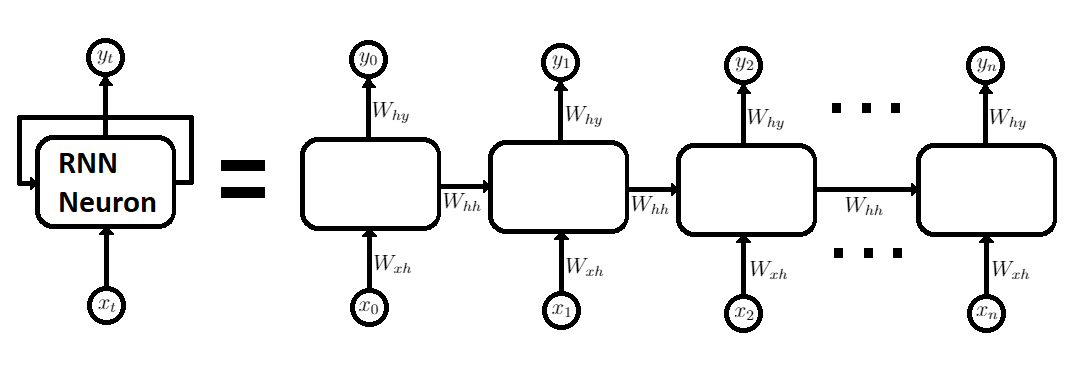
\includegraphics[scale=0.58]{figs/Unrolling.png}
\caption{Schematic description of a Recurrent Neural Network neuron unrolled through time. The information is propagated in a feed-forward manner using the same three weight matrices at each time step.}
\label{fig:unrolling}
\end{figure}
Even though FNNs have outperformed human experts in numerous tasks \cite{NNbH1,NNbH2,NNbH3}, they still lack some fundamental capabilities of the brain. One of which is the ability to remember. To solve this problem Recurrent Neural Networks (RNNs) were introduced. The input features of RNNs are ordered data sequences of varying lengths. RNNs are most prominently capable of understanding and making up meaningful sentences. However, RNNs can also be utilized in physics applications when measurements can be organized as a sequence. For instance, by ordering final state particles of the same type according to their transverse momenta discussed in more detail in Section \ref{sec:feature_selection}. \\
The neurons of an RNN have at least one additional state called the \textit{hidden state}. This state functions as a feedback loop in time connecting the data earlier in the sequences with their successors.
Thus, important information for the context is available at all times. Figure \ref{fig:unrolling} shows the hidden state loop unrolled in time. Each time-step is a copy of the same neuron receiving a different part of the sequence as input $x_i$. Every copy of the neuron is connected with its descendent by the same weight matrix $w_{hh}$. Consequently, the update of the hidden state vector $\vec{h}(t-1)$ to the new hidden state $\vec{h}(t)$ can be expressed as
\begin{equation}
\vec{h}(t) = \Phi(w_{hh} \vec{h}(t-1) + w_{xh} \vec{x})
\end{equation}
where $w_{xh}$ is the weight matrix connecting the input vector $\vec{x}$ with the hidden state and $\Phi$ the activation function. The individual outputs $y_i$ are connected with the current hidden state $h_i$ via the weight matrix $w_{hy}$ and therefore can be calculated as
\begin{equation}
y_i = w_{hy} \cdot h_i
\end{equation}
The training of the weight matrices is performed by the Backpropagation Through Time algorithm (BTT). Similar to the standard Backpropagation algorithm, BTT propagates the gradient backward from the output to the input layer. Additionally, the BTT propagates the gradients also backward in time. \\
While the above-described RNNs can in principle retain information over a long sequence, in practice the calculated gradient quickly vanishes, rendering the training impossible. The solution to this problem comes with the Long Term Short Memory (LSTM) neuron architecture which introduces one more intermediate state called the \textit{cell state}. A LSTM neuron performs four basic iterations at each time step. Firstly the irrelevant parts in the current cell state are forgotten based on the new information and the old hidden state. Then, new information that is relevant for processing the sequence is stored, followed by updating the cell state based on the results obtained. Lastly, the output to the hidden state is computed based on the updated cell state and the new information. \\
The cell state has the advantage that it allows for an uninterrupted flow of the gradients and therefore makes it possible to process long sequential data.

\section{Optimization of Neural Networks}
\label{sec:optimization}
At the base of optimization of Neural Networks is the ``no free lunch theorem''. It states that there is no one single model that works for every problem \cite{patterson2017deep}. The only way to build ANNs with high performance is to try out different optimization algorithms, activation functions, weight initializations, and so forth. Hence, after introducing the performance measure of choice, the most commonly used options will be discussed in this section.

\paragraph{Performance measures} \mbox{} \\

\begin{figure}[H]
\begin{subfigure}{.33\textwidth}
  \centering
  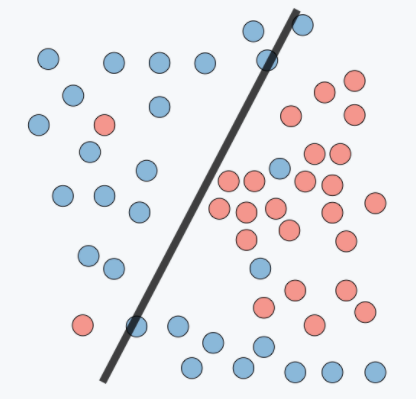
\includegraphics[width=.8\linewidth]{figs/underfitting.png}
  \caption{Underfitting }
  \label{fig:Underfitting}
\end{subfigure}%
\begin{subfigure}{.33\textwidth}
  \centering
  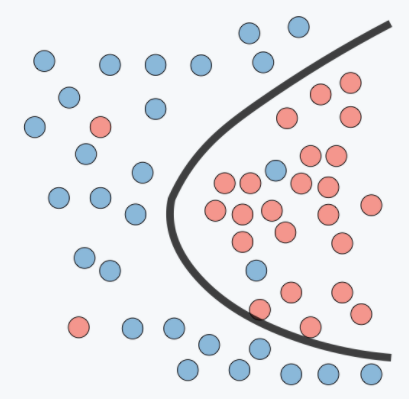
\includegraphics[width=.8\linewidth]{figs/goodfitting.png}
  \caption{Appropriate-fitting}
  \label{fig:Appropriatefitting}
\end{subfigure}
\begin{subfigure}{.33\textwidth}
  \centering
  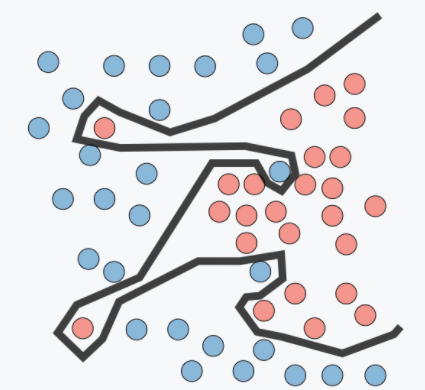
\includegraphics[width=.8\linewidth]{figs/overtraining.png}
  \caption{Overfitting}
  \label{fig:Overfitting}
\end{subfigure}
\caption{Three different models (black) to distinguish the red from the blue circles. \cite{OVPic}}
\label{fig:fitting}
\end{figure}

%Receiver-Operator-Characteristic (ROC) Curve
In this thesis, most of the time binary classification problems are considered where an event either belongs to the signal class or the background class. Therefore, when evaluating the outcome of the classification four cases are possible
\begin{enumerate}[leftmargin=3.5cm]
\setlength{\itemsep}{1pt}
\item[\textbf{True positive (TP):}] The true and the predicted class is signal
\item[\textbf{False negative (FN):}] The true class is signal but the predicted class is background
\item[\textbf{False positive (FP):}] The true class is background but the predicted class is signal
\item[\textbf{True negative (TN):}] The true and the predicted class is background
\end{enumerate}
These quantities can be summarized using the Receiver-Operator-Characteristic (ROC) curve where the signal efficiency ($x = \frac{\text{TP}}{\text{TP}+\text{FN}}$) is plotted against the background rejection ($y =1 - \frac{\text{FP}}{\text{TN}+\text{FP}}$). The separation power of the classifier is then given by $\Gamma$, the Area Under the Curve (AUC) which is the integral under the ROC curve. A model that is capable of distinguishing all signal events from all background events has an AUC of 1. However, in practice, models with such high AUC are very likely to overfit the dataset used during training. Overfitting also called overtraining, schematically depicted in Figure \ref{fig:Overfitting}, occurs when the model is too complex and not only detects subtle patterns of the data but also of the noise. One way of reducing overfitting is to decrease the number of parameters used in the neural network. This is achieved by simplifying its architecture i.e. the number of layers and neurons. On the other hand, a random classifier, which on average gets 50\% of the event classes correctly, achieves an AUC of 0.5. A model that is too simple to parametrize the underlying structure of the data underfits the problem, as shown in Figure \ref{fig:Underfitting}. In the case of Neural Networks there are various ways of avoiding underfitting such as selecting a more complex architecture or adjusting the \textit{learning rate} of the optimization algorithm.

\newpage

\paragraph{Optimization algorithms} \mbox{} \\
Gradient Descent discussed in Section \ref{sec:training} is just one choice of the optimization algorithm. In practice, Gradient Descent is rarely used due to its high computational cost. A very popular variation is the mini batch Stochastic Gradient Descent (SGD) \cite{MainNN}. SGD calculates the weight updates based on a small randomly selected subset of the dataset, called the \textit{batch}.The number of events in the batch the  \text{batch size} and is a hyperparameter of a Neural Network. The full statistics of the dataset is used by calculating the weight updates $m$ times until all events in the dataset were used. The number of batches $m$ is given by batch size divided by the number of events in the total dataset. One evaluation of the weight upgrades on the batch will be refereed to as an \textit{iteration}. The usage of SGD can decrease the computational cost significantly. Furthermore, due to the random nature of the batch selection, the training algorithm can escape local minima in the weight space more easily than the Gradient Descent. \\
Two problems that can similarly slow down the training process are saddle points and plateaus where the gradient and therefore the weight updates can become very small or very large. An optimization algorithm designed to increase the performance of Neural Networks in such situations is the RMSprop \cite{Opti}. This algorithm introduces a constant step size where the direction of the weight update depends on the sign of the gradient. The constant step size is only changed if the previous and the current gradients have the same sign. In this case the step size $v_t$ for the next weight update $w_t$ is given by the previous step size $v_{t-1}$ multiplied with a constant factor $\beta$
\begin{equation}
v_t = \beta v_{t-1}+(1-\beta)(\frac{\partial L}{\partial w})^2
\end{equation}
\begin{equation}
w_t = w_{t-1}-\frac{\alpha}{\sqrt{v_t}} \frac{\partial L}{\partial w}
\end{equation}
where the name giving root mean squared term (RMS) is needed to incorporate mini-batches for the gradient calculation. \\
An optimization algorithm that has been shown to work well for a broad range of applications is the Adaptive Moment Estimation (ADAM) algorithm \cite{Opti}. Like RMSprop it uses $v_t$ term while introducing an additional term $m_t$ called the momentum term. This term ensures a faster convergence by increasing the learning rate for those weights that had a large contribution in the previous step
\begin{equation}
m_t = \beta_2 m_{t-1} + (1-\beta_2) \frac{\partial L}{\partial w}
\end{equation}
where $\beta_2$ is a constant scaling factor. The weight update for ADAM is than given as
\begin{equation}
w_t = w_{t-1}-\frac{\alpha}{\sqrt{\bar{v}_t}} \bar{m_t}
\end{equation}
where $\bar{v_t} = \frac{v_t}{1 - \beta}$ and $\bar{m_t} = \frac{m_t}{1 - \beta_2}$ are bias corrections needed to counteract the initialization to 0. \\
As always in machine learning the best choice of the hyperparameters such as learn rate, scaling factors, and batch size can only be found by testing.

\newpage

\paragraph{Activation functions and Weight initialization}  \mbox{} \\

\begin{figure}[H]
\begin{subfigure}{.5\textwidth}
  \centering
  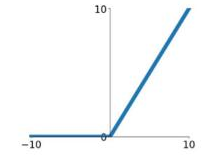
\includegraphics[width=.8\linewidth]{figs/Relu.png}
  \caption{ReLU}
  \label{fig:Relu}
\end{subfigure}%
\begin{subfigure}{.5\textwidth}
  \centering
  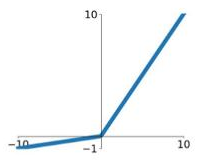
\includegraphics[width=.8\linewidth]{figs/leakyRelu.png}
  \caption{Leaky ReLU}
  \label{fig:LeakyRelu}
\end{subfigure}
\begin{subfigure}{.5\textwidth}
  \centering
  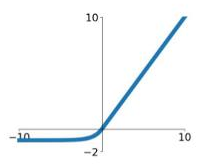
\includegraphics[width=.8\linewidth]{figs/Elu.png}
  \caption{ELU}
  \label{fig:ELU}
\end{subfigure}
\begin{subfigure}{.5\textwidth}
  \centering
  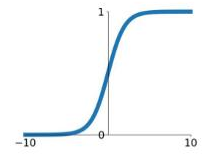
\includegraphics[width=.8\linewidth]{figs/sigmoid.png}
  \caption{Sigmoid}
  \label{fig:Sigmoid}
\end{subfigure}
\caption{Four commonly used activation functions \cite{Acti}}
\label{fig:activfunc}
\end{figure}

Another component of a neural network that can have a big influence on its performance is the activation function. The \textit{rectified linear} (ReLU) activation function, shown in Figure \ref{fig:Relu}, inherits the net input for positive values and evaluates to 0 otherwise. Consequently, the weight updates are easy to compute or cancel completely. This can be an advantage when it comes to computation cost, and a disadvantage if the obtained performance is poor. The \textit{leaky} ReLU activation function (Figure \ref{fig:LeakyRelu}) is similar to ReLU, except for negative values where it returns the net input scaled by a constant $\alpha$. Thus, all weights are updated in each iteration which for some cases improves the performance. The Exponential Linear Unit (ELU), is shown in Figure \ref{fig:ELU}, is very similar to leaky ReLU but has a smooth transition between negative and negative net input values. Its defined as
\begin{equation}
\label{eq:selu}
\text{selu}(z) = \lambda \begin{cases}
z &\text{if}\,\, z < 0 \\
\alpha e^{-z}-\alpha &\text{if}\,\, z \geq 0
\end{cases}
\end{equation}
$\lambda$ is fixed two 1 and $\alpha$ is a tunable parameters. A special version of ELU is the Scaled Exponential Linear Unit (SELU) which was designed to improve the performance of FNNs. The SELU activation function fixes $\alpha$ to 1.6732 and $\lambda$ to 1.0507. The sigmoid activation function (Figure \ref{fig:Sigmoid}) can take values between 0 and 1 and hence is the preferred choice for the output layer where probabilities for the different classes are obtained. Moreover, it's the activation function that is closest to the initial idea of the biological neuron whose output is either 0 or 1. One drawback of the sigmoid activation function is related with its exponential definition (see Section \ref{sec:training}). Calculating exponential functions is much more computationally challenging then computing linear functions like ReLU. \\
Closely related to the selection of the activation function is the choice of the weight initialization. For instance some activation function like SELU require normal distributed weight initialization. The simplest choice would be to initialize all weights and biases to a constant value. However, this leads to the same partial derivative for all weights and thus only one feature could be learned. Therefore, it's not surprising that weight initialization can have a considerable influence on the performance of a neural network. The most popular methods are LeCun, Glorot, and He initialization. These methods draw random values for the initial weights from uniform or normal distribution. They only differ, in upper and lower bounds or standard deviation and mean. The biases, on the other hand, are typically initialized separately either to 0, a small constant value, or 1 in the case of LSTMs.

\paragraph{Regularization} \mbox{} \\
\label{sec:regularization}
The methods and functions described previously all try to increase the performance measure. Another way of improving a Neural Network is to decreasing its overtraining. This process is referred to as \textit{regularization}. The straightforward way of decreasing the overtraining is to reduce the number of parameters. However, removing neurons or entire layers might lead to a completely different training behavior. Two other regularization strategies that avoid changes in the architecture are the Ridge Regression \cite{rigde} and Lasso Regression \cite{lasso} also called $\ell$1 and $\ell$2 regularization. Both introduce additional terms to the loss function. In the case of  Lasso Regression, this term is given by the $\ell$1 norm $\alpha_1 \sum_{i=1}^{n} |w_i|$ where $\alpha_1$ is a new hyperparameter and $w_i$ is the $i^{th}$ weight. A useful property of this regularization is that it tends to eliminate the weights for the least important features. The term of the Ridge Regression is defined as the $\ell$2 norm $\alpha_2 \sum_{i=1}^{n} |w_i|^2$. For large $\alpha_2$, all weights are close to zero, thus reducing the degrees of freedom. \\
Another approach to avoid overtraining is the method of \textit{Dropout} \cite{dropout}. In this method, at each training step, every neuron has a probability $t$ to be temporarily ignored, meaning that it will not forward any output signals to it is successor neurons. Hence, Dropout prevents the neural network to rely too much on specific neurons.

%==============================================================================
\chapter{Neural Network Setup}
\label{sec:NNSetup}
%==============================================================================

Before the Neural Networks introduced in Chapter \ref{sec:ANNs} can be used to analyze the datasets described in Chapter \ref{sec:Samples}, the data needs to be prepared. The preprocessing involves the definition of a dataset splitting strategy to properly treat overfitting and the selection of representative input features for both FNNs and RNNs. Moreover, the transformation of the input features and renormalization of the event weights. \\
For the practical implementation of Neural Networks, the API Keras with Tensorflow as a backend is used throughout this thesis. 


\section{Splitting Strategy}
\label{sec:splitting}

\begin{figure}[H]
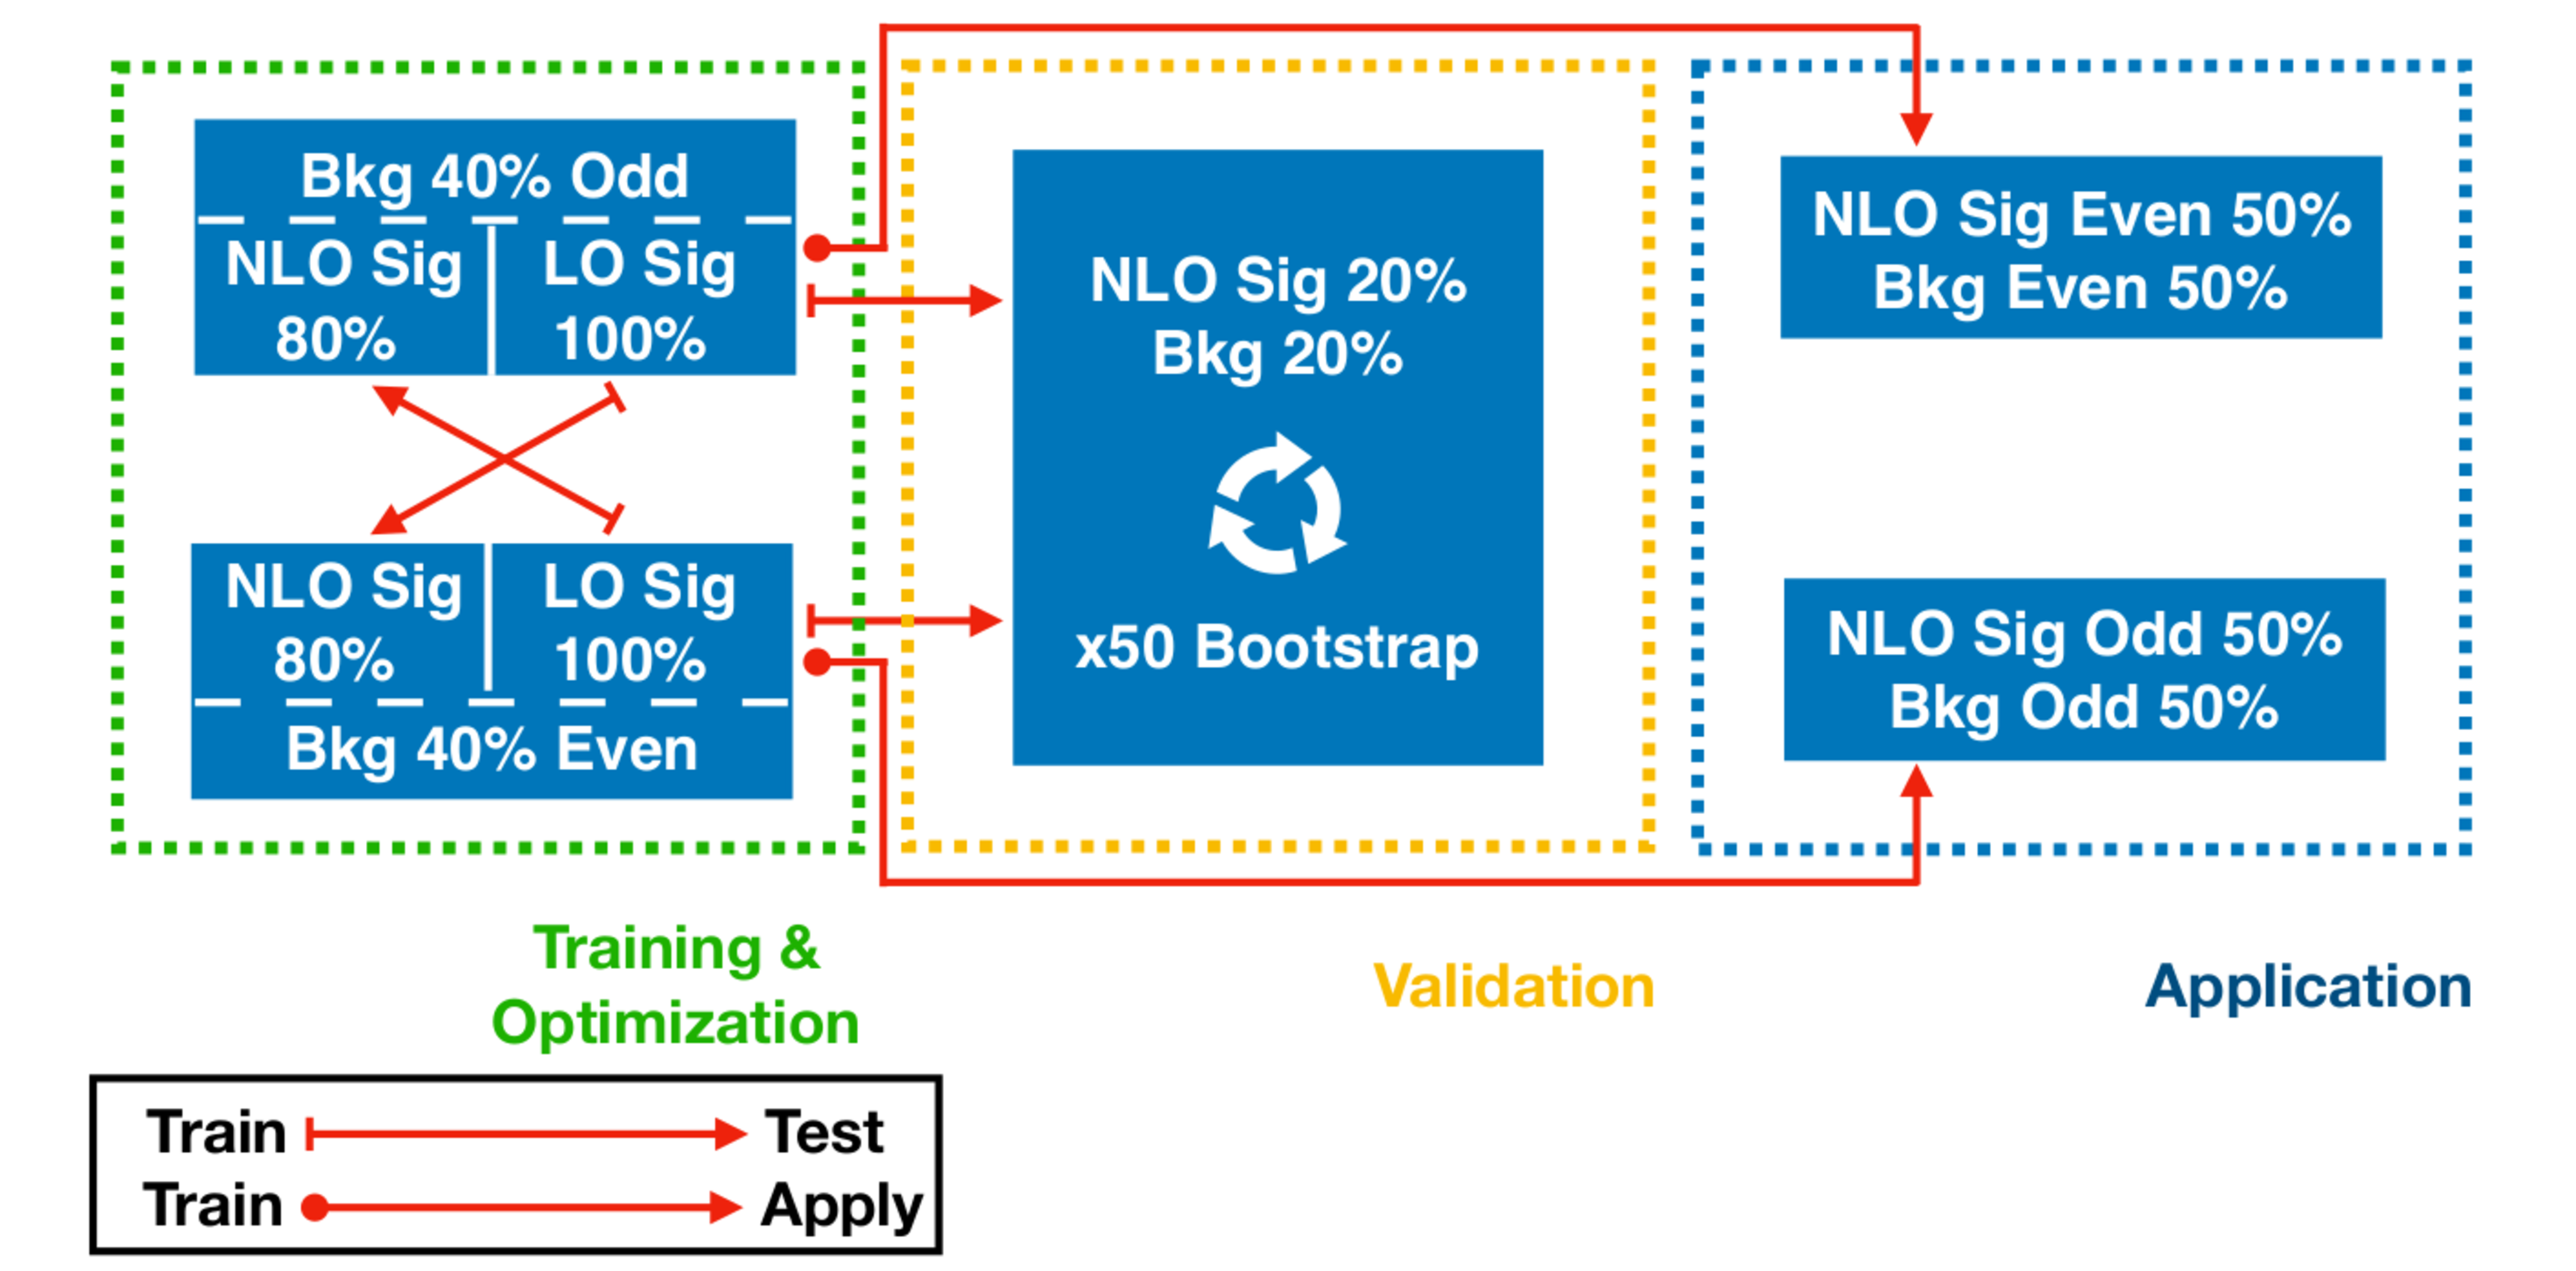
\includegraphics[width=\linewidth , left]{figs/splitting.pdf}
\caption{Splitting strategy that is applied to ensure unbiased estimation of both overtraining and performance. (plot by \"O O\u{g}ul Oncel)}
\label{fig:splitting}
\end{figure}

The two essential quantities of every machine learning model are the performance measure and its overtraining. As discussed in Section \ref{sec:optimization} the performance measure of choice is the AUC ($\Gamma$). It can be evaluated on a single dataset. Overtraining, however, measures how well a model trained on one dataset generalizes to a second dataset. Thus, at least two datasets are needed to evaluate the overtraining of a model. An important side note is that the two datasets need to be orthogonal i.e. they do not have events in common. Therefore, the original dataset is split into two independent datasets called the \textit{training} and the \textit{testing dataset}. As the name suggests, the training of the Neural Network is performed on the training dataset. After all trainable parameters are fixed, the model is tested on the testing dataset. The overtraining $O_v$ as a function of the two obtained AUCs $\Gamma_{\text{test}}$ and $\Gamma_{\text{train}}$ can be expressed as
\begin{equation}
O_v = 1 - \frac{\Gamma_{\text{test}}}{\Gamma_\text{train}}
\label{eq:overtraining}
\end{equation}
The Neural Network with the highest AUC, which has a reasonable $O_v$, typically under 5\%, is considered the best model. The detailed strategy to discover the best model is described in chapter \ref{sec:Results}. The optimization relies on training numerous models with different hyperparameters and architectures. However, since the same testing dataset is exploited multiple times, this approach introduces a bias into the overfitting measurement. To compensate for this, a third orthogonal dataset called the \textit{validation dataset} is introduced. Similar to the testing dataset, it is spared during training and additionally also remains unused during the optimization. Only after all hyperparameters are fixed, the $\Gamma_{\text{validation}}$ is calculated. Thus, allowing for unbiased estimation of $O_v$. Equation \ref{eq:overtraining} needs to be adjusted by replacing $\Gamma_{\text{test}}$ with $\Gamma{\text{validation}}$, for the final evaluation of the overtraining. The error of the obtained overfitting is then evaluated by generating multiple versions of the validation dataset and evaluating the AUC on all of them. The different versions of the validation dataset are generated using random sampling with replacement referred to as \textit{bootstrapping}. \\
The background datasets available of the four-top-quark analyses are split into 20\% validation dataset and 80\% for testing and training. The segmentation of the dataset containing 80\% of all background events is performed by splitting on the event number\footnote{The event number is the position of the event in the dataset.} (even or odd). The obtained datasets are referred to as the \textit{even} and the \textit{odd dataset}. This procedure is applied for each background dataset individually such that the three final datasets have a proper number of events for each process. The $t\bar{t}t\bar{t}$ signal dataset, since it holds events calculated both at leading order and next-to-leading order, is treated differently. All LO events are used for training to avoid the negative event weights problem, which will be discussed in section \ref{sec:transformation}. The NLO events are split into 80\% testing dataset and 20\% for validation dataset. The complete splitting strategy is summarized in Figure \ref{fig:splitting}. The application step indicated corresponds to further studies of the $t\bar{t}t\bar{t}$ process performed on the NLO events. As the red arrows imply, two Neural Networks with the same hyperparameters are trained. The first one uses the even dataset as the training dataset and the odd dataset as the testing dataset (yielding $\Gamma_{\text{even}}$). The definition of the testing and training dataset is interchanged for the second Neural Network (yielding $\Gamma_{\text{odd}}$). The combined AUC $\Gamma_{\text{total}}$ can be determined as
\begin{equation}
\Gamma_{\text{total}} = \frac{\Gamma_{\text{even}} + \Gamma_{\text{odd}}}{2}
\end{equation}
This scheme ensures that the final performance measure $\Gamma_{\text{total}}$ is independent of the concrete choice of the training and testing datasets. 

\section{Feature Selection}
\label{sec:feature_selection}

The selection of input features is crucial to obtain a Neural Network with a high AUC. The features selected have to discriminate the signal process well from the background processes. If to many or irrelevant features are selected, the training of the Neural Network is slow down which in turn can lead to decreased performance. The usage of prior information about the problem, such as the different physical characteristics of a processes, can be used as a guideline to find good separating features. In the case of the $t\bar{t}t\bar{t}$ process,
it is known that the final state has a high jet and b-jet multiplicity (cf. Section \ref{sec:fourtops}). As can be seen in Figures \ref{fig:MV2c10} to \ref{fig:dRbb} these properties are reflected in the number of jets ($n_{j}$) and the b-tagging score $\sum w_{\text{MV2c10}}$. To be more precise $\sum w_{\text{MV2c10}}$ is calculated by assigning each jet in the event a weight depending on its MV2c10 score. The weights can take values between 1, if the jet passes non of the working points, and 5, if jet passes all of the working points. \\
In practice, resolution and detector effects can smear out expected characteristics. Therefore, it is necessary to validate which features increase $\Gamma_{\text{total}}$. As the first figure of merit, the ranking of features provided by a boosted decision tree \cite{BDT} is adopted. The ranking is derived by counting how often a feature is used to split decision tree nodes, and by weighting each split occurrence by the separation gain squared, it has achieved \cite{TMVA}. To ensure that the highest-ranking features are also well suited for Neural Networks, a study using an iterative removal algorithm is performed. This algorithm aims to find the best $k$ features out of a set of $m$ features, by training $m$ Neural Networks with the same hyperparameters. Each of the Neural Networks is trained without one of the $m$ features. The feature that had the least impacted on the AUC is removed. This process is repeated until only $k$ features remain.
The 18 features selected in this manner are summarized in table \ref{tab:feature_selection}, together with the respective BDT ranking scores. As previously mentioned, $N_j$ and $\sum w_{\text{MV2c10}}$ are two of the highest-scoring features alongside the angular distance features $\Delta R(x,y)$ which are calculated according to
\begin{equation}
\Delta R(x,y) = \sqrt{(\eta_x - \eta_y)^2 + (\phi_x - \phi_y)^2}
\end{equation}
where x and y are two particle types. An example of an angular distance distribution is shown in Figure \ref{fig:dRbb}. $\Delta R(b,b)_{\text{min}}$ refers to the minimum angular distance between any b-jet pair. \\

\begin{table}[H]
\begin{tabular}{|l|l|l|}
\toprule
Feature & Definition & BDT ranking score \\
\midrule \midrule
$\sum w_{\text{MV2c10}}$ & Sum of b-tagging weights of MV2c10 & 0.114 \\
$\Delta R(l,l)_{\text{min}}$ & Maximum angular distance between any lepton pair & 0.063 \\
$p_{\text{T}}^{j,0}$ & $p_{\text{T}}$ of the leading jet & 0.063 \\
$E_{\text{T}}^{\text{miss}}$ & missing transverse energy & 0.059 \\
$N_j$ & Jet multiplicity & 0.059 \\
$p_{\text{T}}^{\ell,0}$ & $p_{\text{T}}$ of the leading lepton & 0.059 \\
$p_{\text{T}}^{b,0}$ & $p_{\text{T}}$ of the leading b-jet & 0.058 \\
$\Delta R(b,b)_{\text{min}}$ & Minimum angular distance between any b-jet pair & 0.055 \\
$p_{\text{T}}^{j,5}$ & $p_{\text{T}}$ of the fifth highest jet & 0.055 \\
$\Delta R(l,b)_{\text{max}}$ & Maximum angular distance between any lepton and b-jet & 0.054 \\
$\Delta R(l,j)_{\text{min}}$ & Minimum angular distance between any lepton and jet & 0.051 \\
$H_{\text{T}}^{0}$ & Scalar sum of all lepton and jet $p_{\text{T}}$'s excluding the leading jet & 0.049 \\
$p_{\text{T}}^{\ell,1}$ & $p_{\text{T}}$ of the sub-leading lepton & 0.049 \\
$\sum_l \Delta R(l,l)$ & Sum of all angular distance between any lepton pair & 0.040 \\
$p_{\text{T}}^{j,1}$ & $p_{\text{T}}$ of the sub-leading jet & 0.039 \\
$\Delta R(l,l)_{\text{max}}$ & Maximum angular distance between any lepton pair & 0.039 \\
$\Delta R(l,b)_{\text{min}}$ & Minimum angular distance between any lepton and b-jet & 0.039 \\
$\phi^{\ell,0}$ & $\phi$ of the leading lepton & 0.038 \\
\bottomrule
\end{tabular}
\caption{The 18 selected features for the FNNs with there respective BDT ranking score}
\label{tab:feature_selection}
\end{table}


The approach chosen to select features for the RNN is different and is loosely inspired by \cite{RNNSel}. The four momenta and the decaying angles of the reconstructed objects in the final state are used directly as input features. If multiple particles of the same type are present in the final state of an event, this particles are sorted according to their $p_{\text{T}}$. Thus, an input feature such as the pseudorapidity of any jet $\eta_j$ is a $p_{\text{T}}$ sorted sequence of length $N_j$ where $n_j$ is the number of jets observed in the event.  In practice, all input feature sequences in the same event have to have the same length. This is accomplished by padding sequences that do not have the desired length with zeros. In addition to the features described above, some high-level features, such as $\sum w_{\text{MV2c10}}$, are selected. The combination of the two types of features was shown to increase performance in several applications \cite{SpeFea1,SpeFea2}. The input features selected are $\phi$, $\eta$, $p_{\text{T}}$ of electron, muons and jets as well as $E_{\text{T}}^{\text{miss}}$, $\phi_{\text{T}}^{\text{miss}}$, $N_j$ and $\sum w_{\text{MV2c10}}$. All features for FNNs and RNNs are shown in detail in the Appendix \ref{ap:Input}.

\newpage

To have some kind of feature selection, a small $\ell$1 regularization term is applied to the RNN. As briefly mentioned in Section \ref{sec:optimization}, this regularization tends to eliminate connections to the least important features. Thus an automatic feature selection is provided, which suppresses redundant information.

%\begin{figure}[H]
%\begin{minipage}[t]{.5\linewidth}
%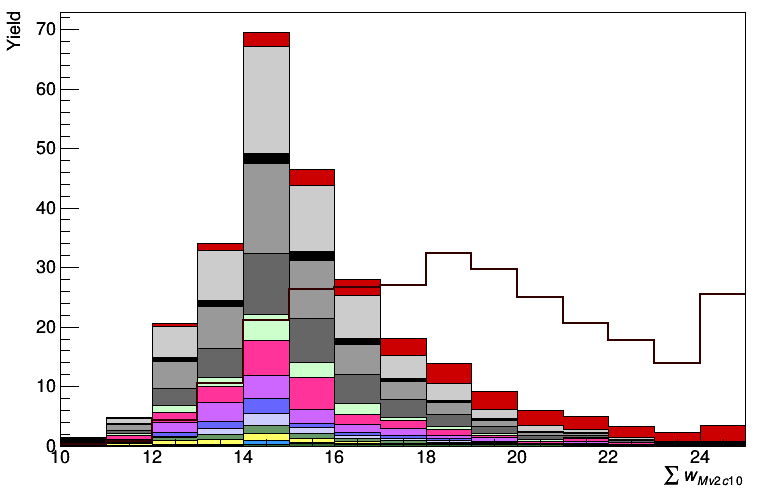
\includegraphics[width=\linewidth]{figs/features/MV2c10.png}
%\caption{Sum of the continuous MV2c10 b-tagging score}
%\label{fig:MV2c10}
%\end{minipage}
%\hspace{.01\linewidth}
%\begin{minipage}[t]{.5\linewidth}
%\includegraphics[width=\linewidth]{figs/features/nJets.png}
%\caption{Jet multiplicity}
%\label{fig:nJets}
%\end{minipage}
%
%
%\begin{minipage}[t]{.5\linewidth}
%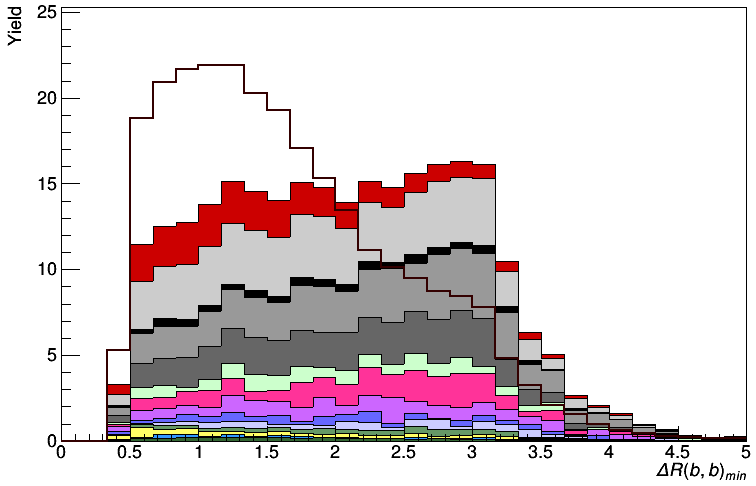
\includegraphics[width=\linewidth]{figs/features/dRbbmin.png}
%\caption{minimum angular distance between any b-jet pair}
%\label{fig:dRbbmin}
%\end{minipage}
%\hspace{.01\linewidth}
%\begin{minipage}[t]{.5\linewidth}
%\centering
%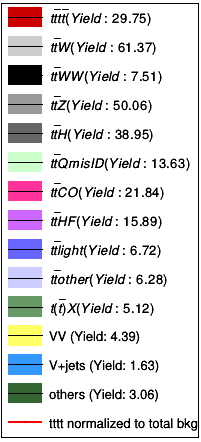
\includegraphics[width=0.3\linewidth]{figs/features/legende.png}
%\caption{Legend}
%\label{fig:Legend}
%\end{minipage}
%
%\end{figure}


\begin{figure}[H]
\begin{subfigure}{.5\textwidth}
  \centering
  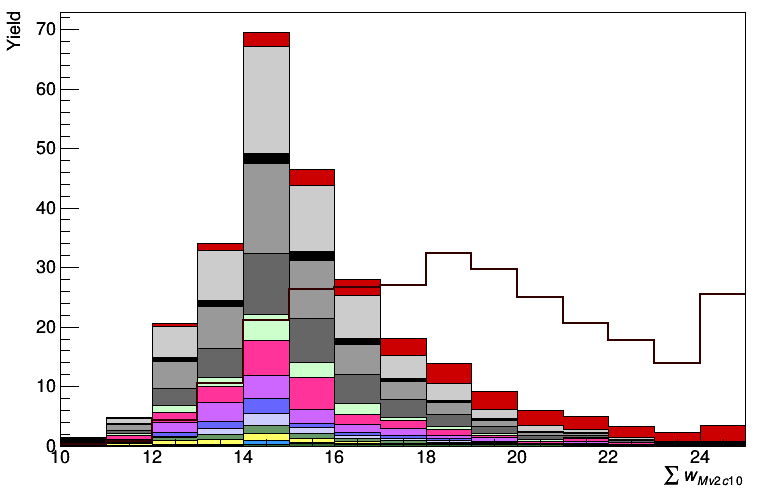
\includegraphics[width=.99\linewidth]{figs/features/MV2c10}
  \caption{Sum of b-tagging weights of MV2c10}
  \label{fig:MV2c10}
\end{subfigure}%
\begin{subfigure}{.5\textwidth}
  \centering
  \includegraphics[width=.99\linewidth]{figs//features/nJets}
  \caption{Jet multiplicity}
  \label{fig:nJets}
\end{subfigure}
\begin{subfigure}{.5\textwidth}
  \centering
  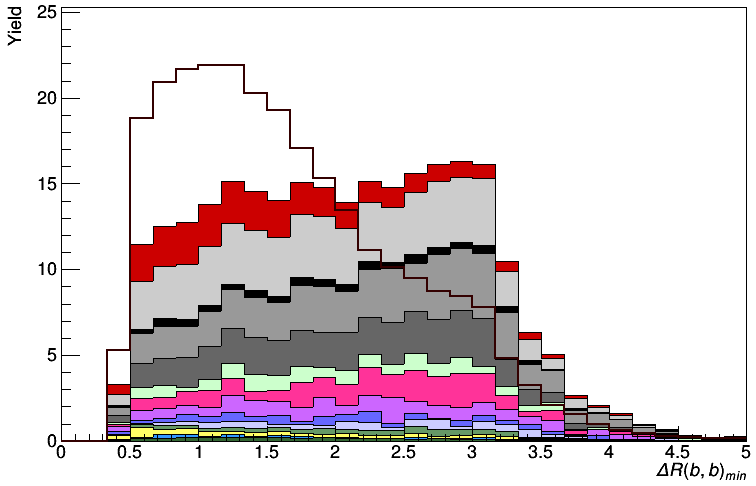
\includegraphics[width=.99\linewidth]{figs/features/dRbbmin}
  \caption{minimum angular distance between any b-jet pair}
  \label{fig:dRbb}
\end{subfigure}%
\begin{subfigure}{.5\textwidth}
  \centering
  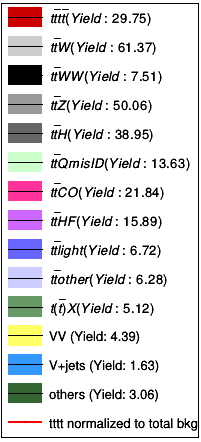
\includegraphics[width=.29\linewidth]{figs/features/legende}
  \caption{Legend}
  \label{fig:LegendwY}
\end{subfigure}
\caption{Three of the most discriminating features of the FNN study. The last bin in all distribution contains additionally the events which fall into bins above the maximum x-axis range.}
\label{fig:BestFeatures}
\end{figure}


\section{Feature Transformation and Event Weight Treatment}
\label{sec:transformation}

As discussed in Section \ref{sec:training}, the backpropagation algorithm calculates the gradients of the loss function for each weight, starting from the output layer and working backward to the input layer. Each gradient of the current step, therefore, depends on the gradients derived in the previous step. Thus, when the selected input features have small numerical values, the gradients start to \textit{vanish} \cite{MainNN}, leaving the weights virtually unchanged. On the other hand, if the features have big numerical values, the gradients can become very large, leading to the \textit{exploding gradient problem} \cite{MainNN}. Both cases can hinder the convergence of the Neural Network. One way of dealing with this problem is to transform all input features to normal distributions i.e. 0 mean and a variance of 1, before feeding them to the Neural Network. This transformation is crucial. Neural Networks trained without it show an up to 0.2 decreased AUC compared to the same Neural Networks with transformed input features. Additionally, the SELU activation function can be utilized to normalize the neuron outputs at each layer.\\

\begin{figure}[H]
\begin{subfigure}{.5\textwidth}
  \centering
  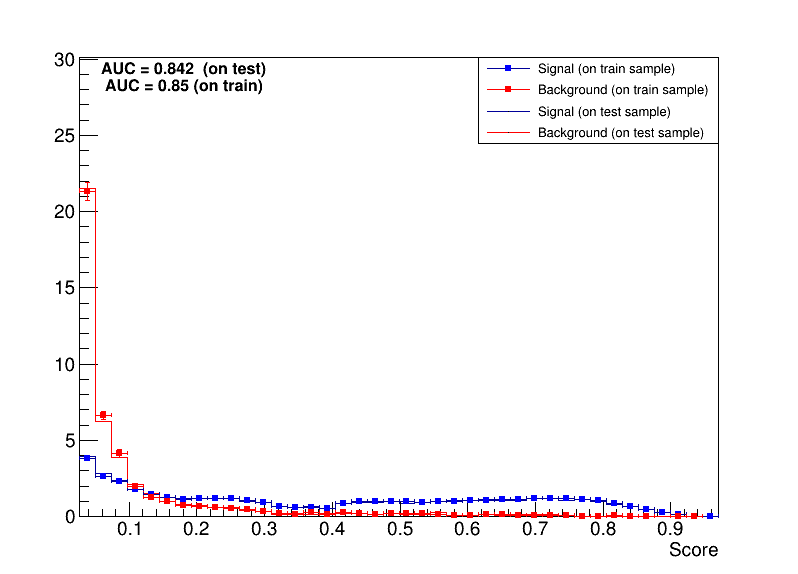
\includegraphics[width=.99\linewidth]{figs/Score_w_weights}
  \caption{Event weights applied}
  \label{fig:ScoreWeights}
\end{subfigure}%
\begin{subfigure}{.5\textwidth}
  \centering
  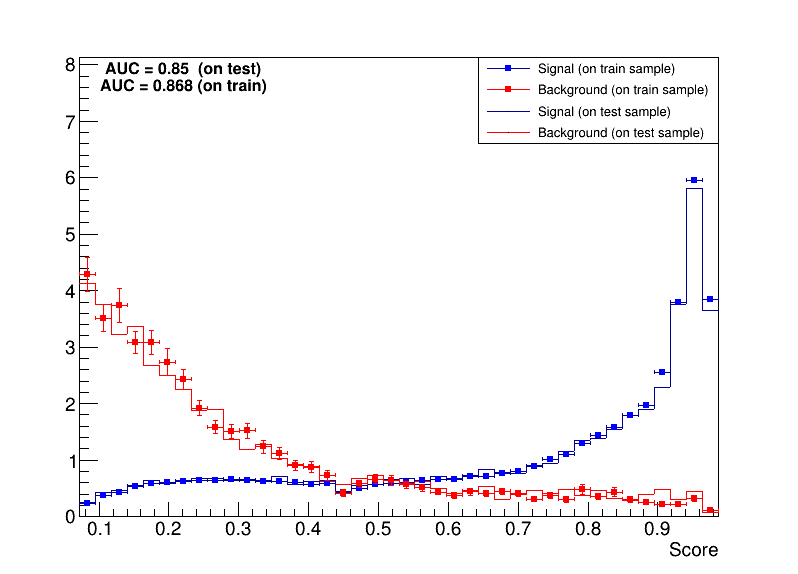
\includegraphics[width=.99\linewidth]{figs/Score_reweighted}
  \caption{Renormalization event weights applied}
  \label{fig:ScoreRenormed}
\end{subfigure}
\caption{The difference in classification between a Neural Network trained with and without renormalization event weights.}
\label{fig:ScoreWvsR}
\end{figure}

Event weights are interpreted as probabilities in Neural Networks. This probabilities are multiplied with the loss function at each training step.
When the event weights, introduced in Chapter \ref{sec:EventSelection}, are very small or very large, the he training of Neural Networks are effect by the vanishing and exploding gradient problem. This is because gradients are calculated based on the loss function. To avoid very large and very small event weights, a renormalization is applied such that the sum of all weighted signal training events equals the sum of all weights of the background training events, following the approach described in \cite{TMVA}. The renormalized event weight are exclusively used during training. \\
The score distributions\footnote{The y-axis of the displayed distributions shows the number of events normalized to $\frac{dN}{dx}$ where $dN$ is the total number of events and $dx$ is given by one over the number of bins.} shown in Figure \ref{fig:ScoreWvsR} are the probabilities assigned by the Neural Network for a given event to be a signal event. The red dots and lines represent events that truly originate from $t\bar{t}t\bar{t}$ events, while the blue dots and lines represent events that truly originate from background processes. The solid lines denote the score obtained for the training dataset while the dots denote the score obtained on the testing dataset. A perfect classifier would be a classifier for which all signal events are in the first bin, and all background events are in the last bin. \\
Figure \ref{fig:ScoreWeights} shows the score of a Neural Network trained without the renormalization applied. The Neural Network focuses on the background events since the total background Yield (228) is much higher than the signal Yield (30). The same Neural Network is used to obtain the score shown in Figure \ref{fig:ScoreRenormed}, the only difference being the applied renormalization of the weights. The classification with renormalization weights clearly separates background and signal events and ultimately results in an higher AUC. \\
 All negative events weights are set to 0 during the training since the usual interpretation of the event weight as probabilities can not be applied. A problem referred to as the \textit{negative weight problem} \cite{nWeights}.
%==============================================================================
\chapter{Results}
\label{sec:Results}
%==============================================================================

Based on the studies and methods described in the previous chapters, this chapter presents the four-top-quark signal classification results using Deep Neural Networks. In the first section (Section \ref{sec:FNN_results}), different hyperparameters and ingredients of Feedforward Neural Networks for a signal vs. all background are studied. Section \ref{sec:Multi} explores the potential and the implications of a training of Feedforward Neural Networks with multiple different background classes. In Section \ref{sec:RNN_results}, the construction and the obtained signal discrimination of Recurrent Neural Networks will be presented.
Section \ref{sec:CPUGPU} presents a study on the training duration of Neural Networks on both central processing units (CPUs) and graphics processing unit (GPUs). The last section (Section \ref{sec:TwoHadTop}) is concerned with the reconstruction of two hadronically decaying top quarks; in order to improve the discrimination of $t\bar{t}t$ in the four-top-quark analysis. \\
The statements made about Neural Networks in the following sections are not necessarily transferable to other applications. The influence of hyperparameters and other ingredients of Neural Networks depends on the application and size of the dataset used.

\section{Signal Classification using Feedforward Neural Networks}
\label{sec:FNN_results}

The strategy chosen to obtain an FNN that discriminates the $t\bar{t}t\bar{t}$ signal well from the background processes seeks to optimize the structure of the Neural Network and tune its most important hyperparameters. The correlation between different ingredients of the Neural Networks is taken into consideration by investigating several parameters at the same time. To limit the number of Neural Networks that need to be trained to a reasonable amount, only parameters with presumably highly correlations are varied simultaneously. Furthermore, unless stated otherwise, all performance measures obtained are based on a \textit{binary classification} approach. In binary classification, only two classes are considered a signal and a background class. The AUC of the current classification is calculated at each Epoch on the testing set. The FNNs are trained until five consecutive Epochs did not improve the AUC, but at least for 80 Epochs. The AUCs quoted in the following sections are the mean of the two Neural Networks trained ($\Gamma_{\text{total}}$) unless stated otherwise. As described in Chapter \ref{sec:NNSetup}, the 18 input features are first transformed into normal distributions and then reweighted before they enter the input layer.

\paragraph{Architecture} \mbox{} \\

The first choice that has to be made is the number of parameters, also called the \textit{size}, and the number layers of the Neural Network, referred to as the \textit{depth}. As discussed in Chapter \ref{sec:Deep_learning} , the architecture has to be complex enough to model the problem and not too complex to avoid overtraining. \\
The number of parameters needed for the $t\bar{t}t\bar{t}$ application is investigated by using fully connected layers and can be calculated according to Equation \ref{eq:NumPara}. The parameters are distributed to the layers such that the number of neurons in progressive layers declines. Additionally, the number of neurons in a hidden layer is required to be at least 25\% the number of neurons in the input layer ($18 \times 0.25 = 4.5 \approx 5$), following the approach described in \cite{RNNSel}. Since the dataset is small for a deep learning application, the number of hidden layers is kept small. \\
Neural Networks considered had 200 to 70000 tunable parameters and are evenly spread over the three orders of magnitude studied. For each size investigated, 10 Neural Networks with 1 to 10 hidden layers are trained. The only exceptions are Neural Networks with less than 1000 parameters, where the number of neurons would have fallen below 5. For Neural Networks with these sizes, only a maximum depth of 5 was considered. All other ingredients are kept constant. \\


\begin{figure}[H]
\centering
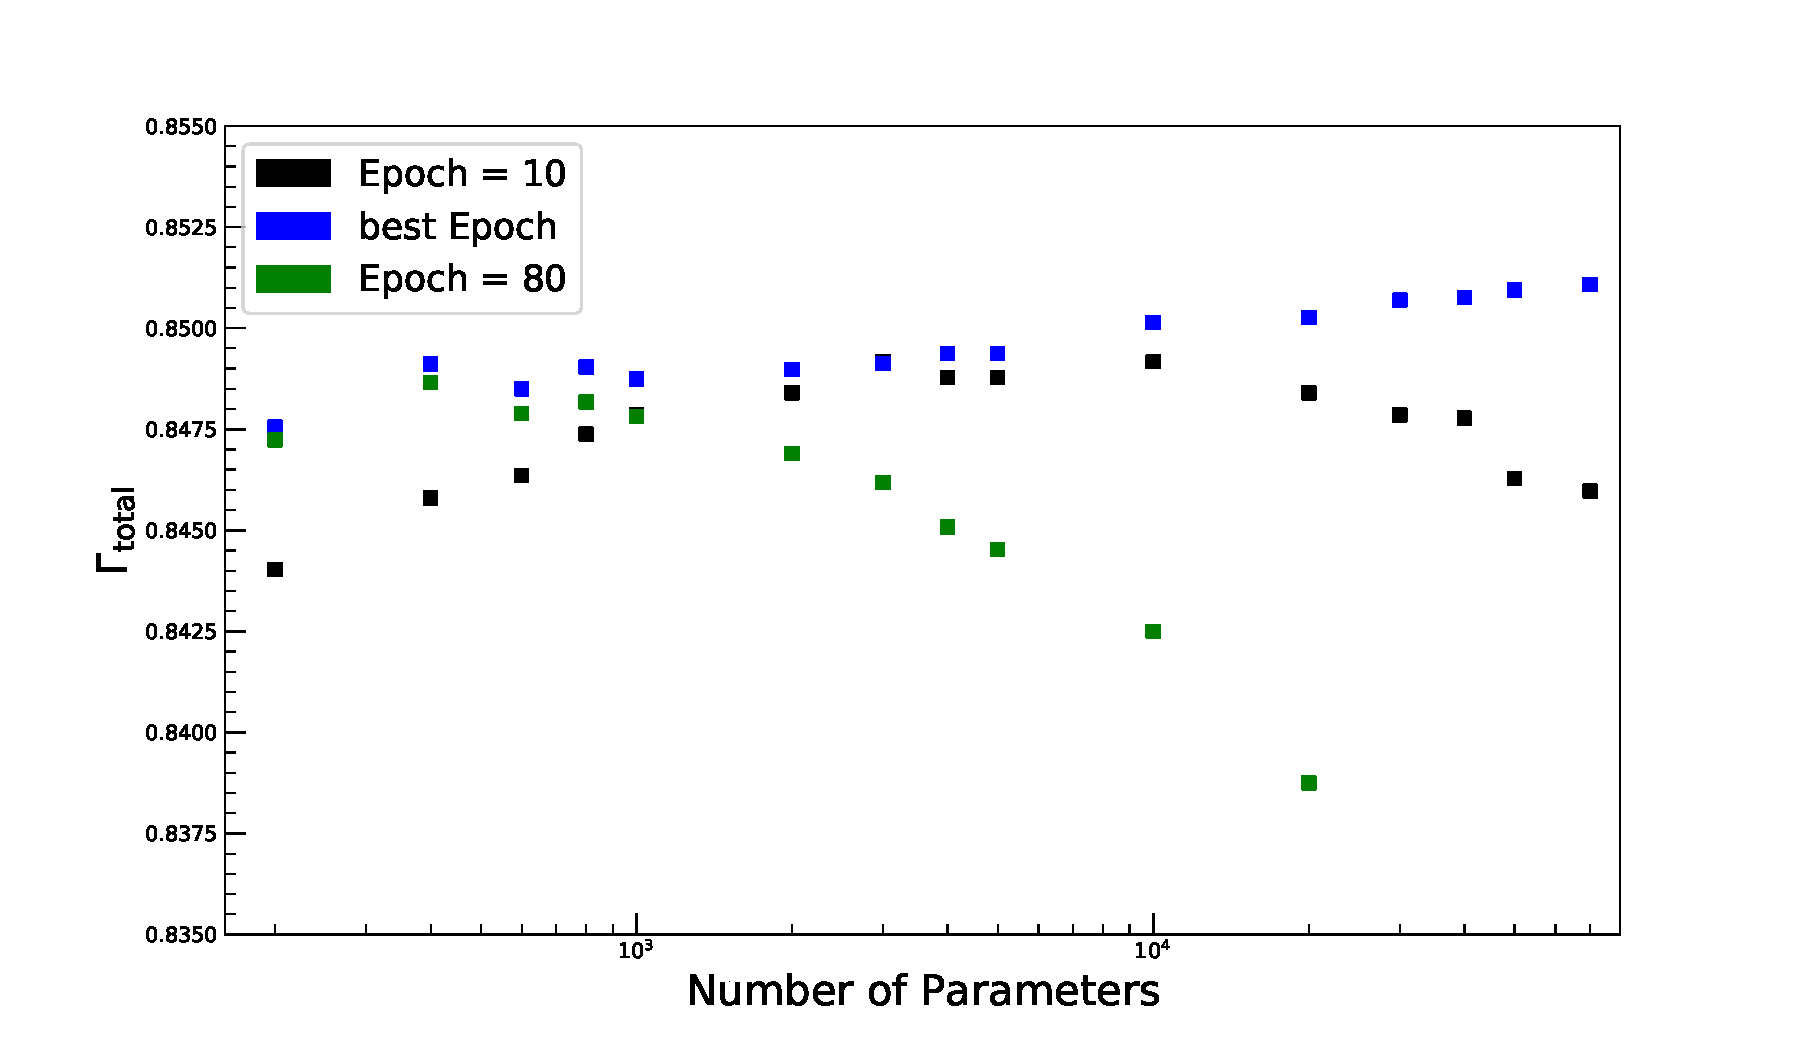
\includegraphics[width=\linewidth]{figs/FNN/AucPara_Fixed}
\caption{The averaged AUCs of FNNs with different number of parameters where the training is stopped after 10, 80 and at the best-performing Epoch. The average includes the AUCs of the 4 best-performing Neural Networks of different depth.}
\label{fig:AucPara}
\end{figure}


Figure \ref{fig:AucPara} shows the result of the search for the number of parameters where $\Gamma_{\text{total}}$ is the average of the 4 best-performing Neural Networks differing in the layer configuration. For all sizes, the standard deviation of the average is smaller than 0.001. For the blue squares, the Epoch with the highest AUC for each Neural Network was selected, whereas, for the black and green, the AUC at Epoch 10 and 80 is reported. \\
The $\Gamma_{\text{total}}$ for the best Epoch slightly increases with higher number of parameters. For Neural Networks with more than 10000 parameters, the performance gain per additional trainable parameter is minor, indicating that the current number of parameters is sufficient to obtain a reasonable separation between signal and background events. In the case of Neural Networks with few parameters, every weight needs to be fine-tuned so as to obtain the best possible performance, which can take several Epochs. On the other hand, for Neural Networks with many parameters, not all information available to a neuron is important. The learning process to identify which of the available information is key to obtain a good training result can also take several iterations. These behaviors are reflected in the distribution of the training results evaluated at Epoch 10 which show AUCs close to the best observed AUC only for Neural Networks of intermediate size.
The Neural Networks evaluated at Epoch 80 show a strong decrease in the $\Gamma_{\text{total}}$ (obtained on the test sets) with the number of parameters, indicating overtraining. The tendency of large Neural Networks to have high overtraining is especially apparent in Figure \ref{fig:OvPara} for high Epochs. However, when the AUC is calculated at the optimal Epoch, this dependency is significantly attenuated. \\

\begin{figure}[H]
\centering
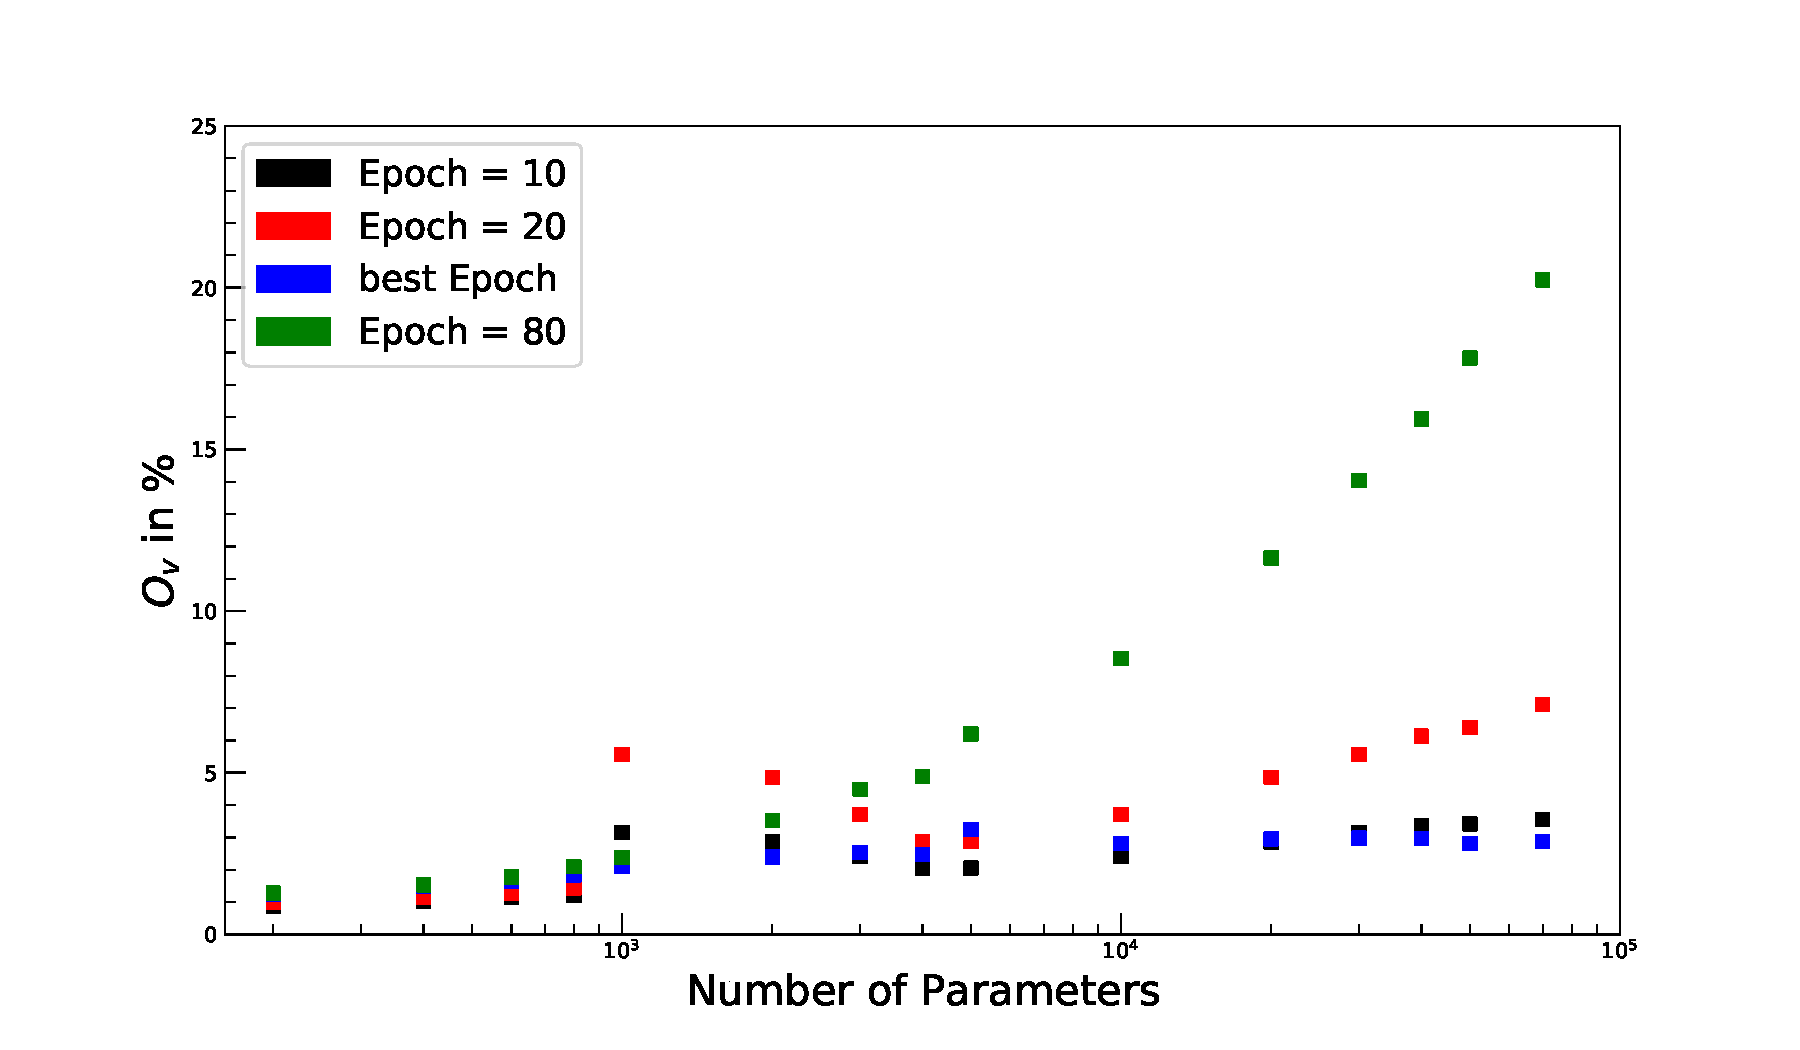
\includegraphics[width=\linewidth]{figs/FNN/OvPara_Fixed}
\caption{The average overtraining for different FNN configurations. The training is stopped after 10, 20, 80 and at the best-performing Epoch. The average includes the overtrainings of the 4 best-performing Neural Networks of different depth.}
\label{fig:OvPara}
\end{figure}

\begin{figure}[H]
\centering
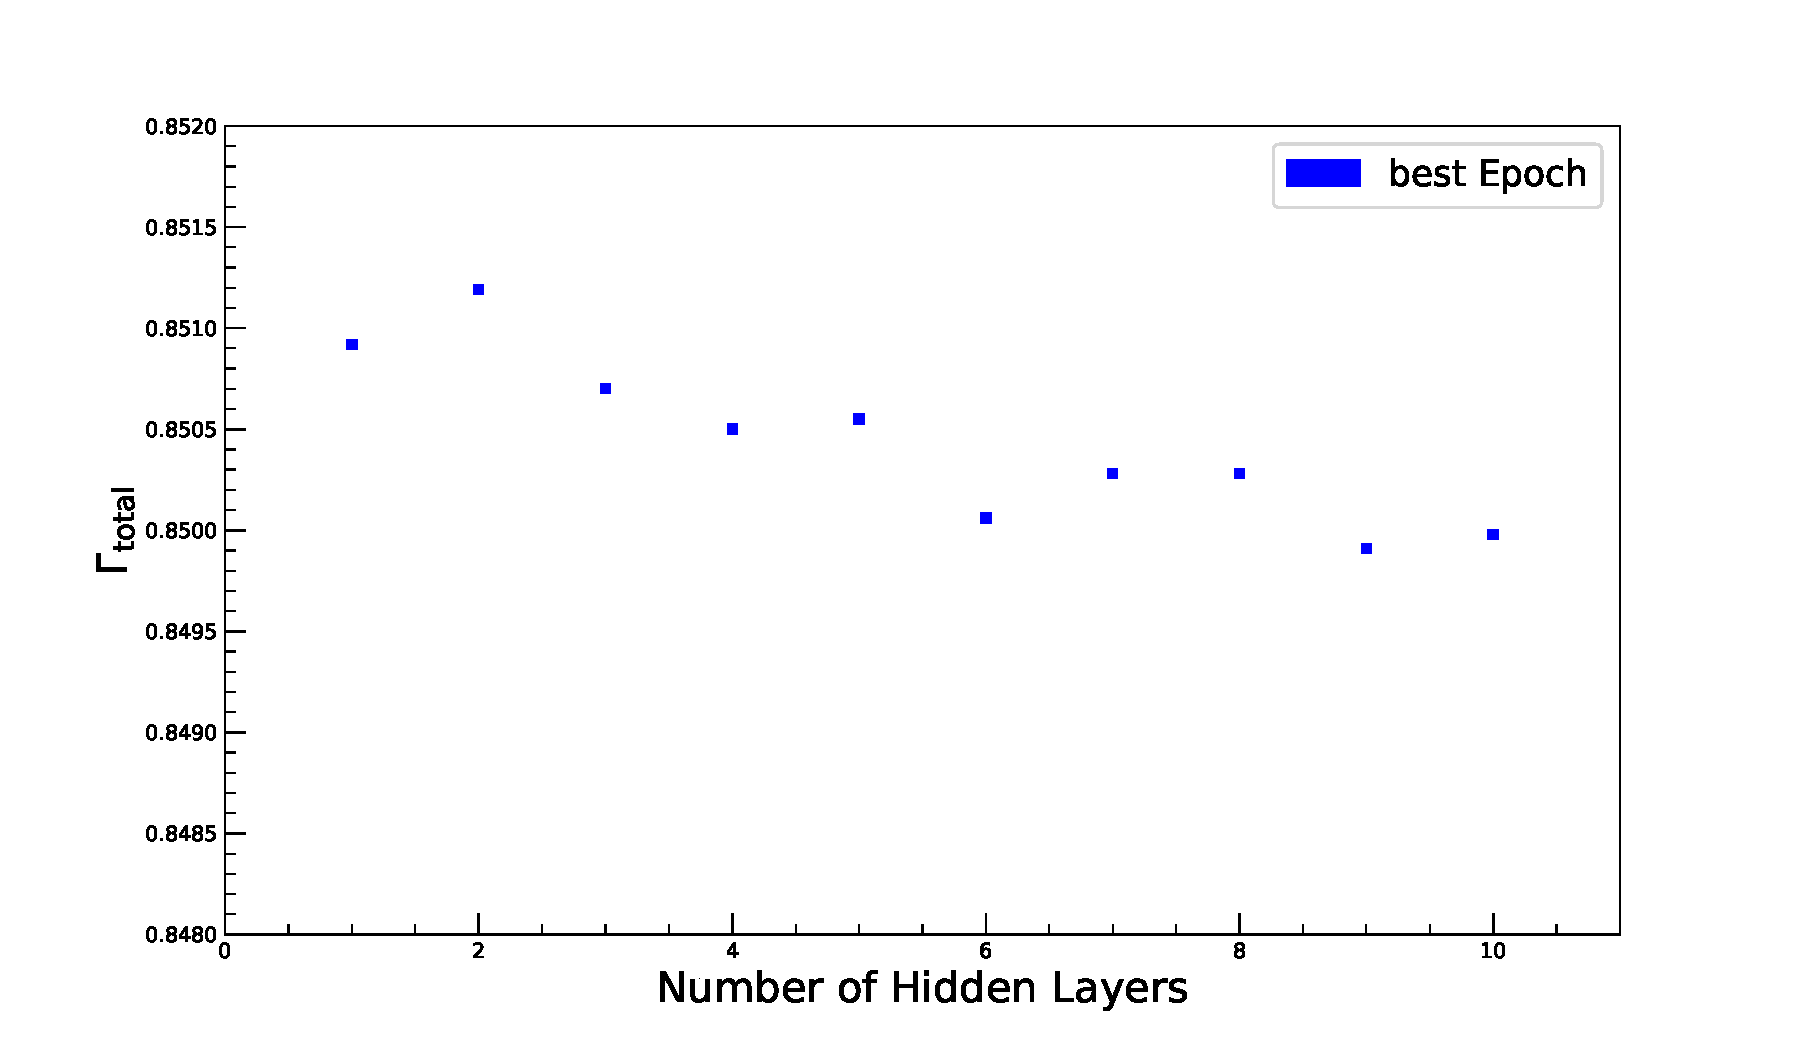
\includegraphics[width=\linewidth]{figs/FNN/Aver_LayersAuc}
\caption{The average AUC for FNNs with different numbers of hidden layers. The average includes the AUCs of the 4 best-performing Neural Networks of different size.}
\label{fig:AucLayers}
\end{figure}

\newpage

In Figure \ref{fig:AucLayers}, the average AUCs of Neural Networks with different numbers of hidden layers are shown. The average includes the 4 best-performing Neural Networks of different size. The FNNs showing the highest AUC are models with low numbers of hidden layers, especially those with two layers. The overtraining was observed to be independent of the number of hidden layers. \\
The overall performance gained by varying the number of parameters and layers is small compared to the performance gained by hyperparameter tuning. This is because the selected optimization algorithm Adam is very stable in its final performance, in combination with a reasonable initial learning rate. A cross-check using mini-batch Stochastic Gradient Descent (SGD) showed that, for this algorithm, the performance does depend more on the number of parameters. \\
Summarizing the obtained results, it can be stated that a Neural Network for hyperparameter tuning should have more than 10000 parameters to ensure high flexibility and less than 30000 to avoid high overtraining.
For the studies on learning rate, activation function, and weight initialization, a Neural Network with 20000 parameters and 2 hidden layers is selected. Its overtraining is shown in Figure \ref{fig:RegionPara} together with the overtraining of other Neural Networks in the region of interest.


\begin{figure}[H]
\centering
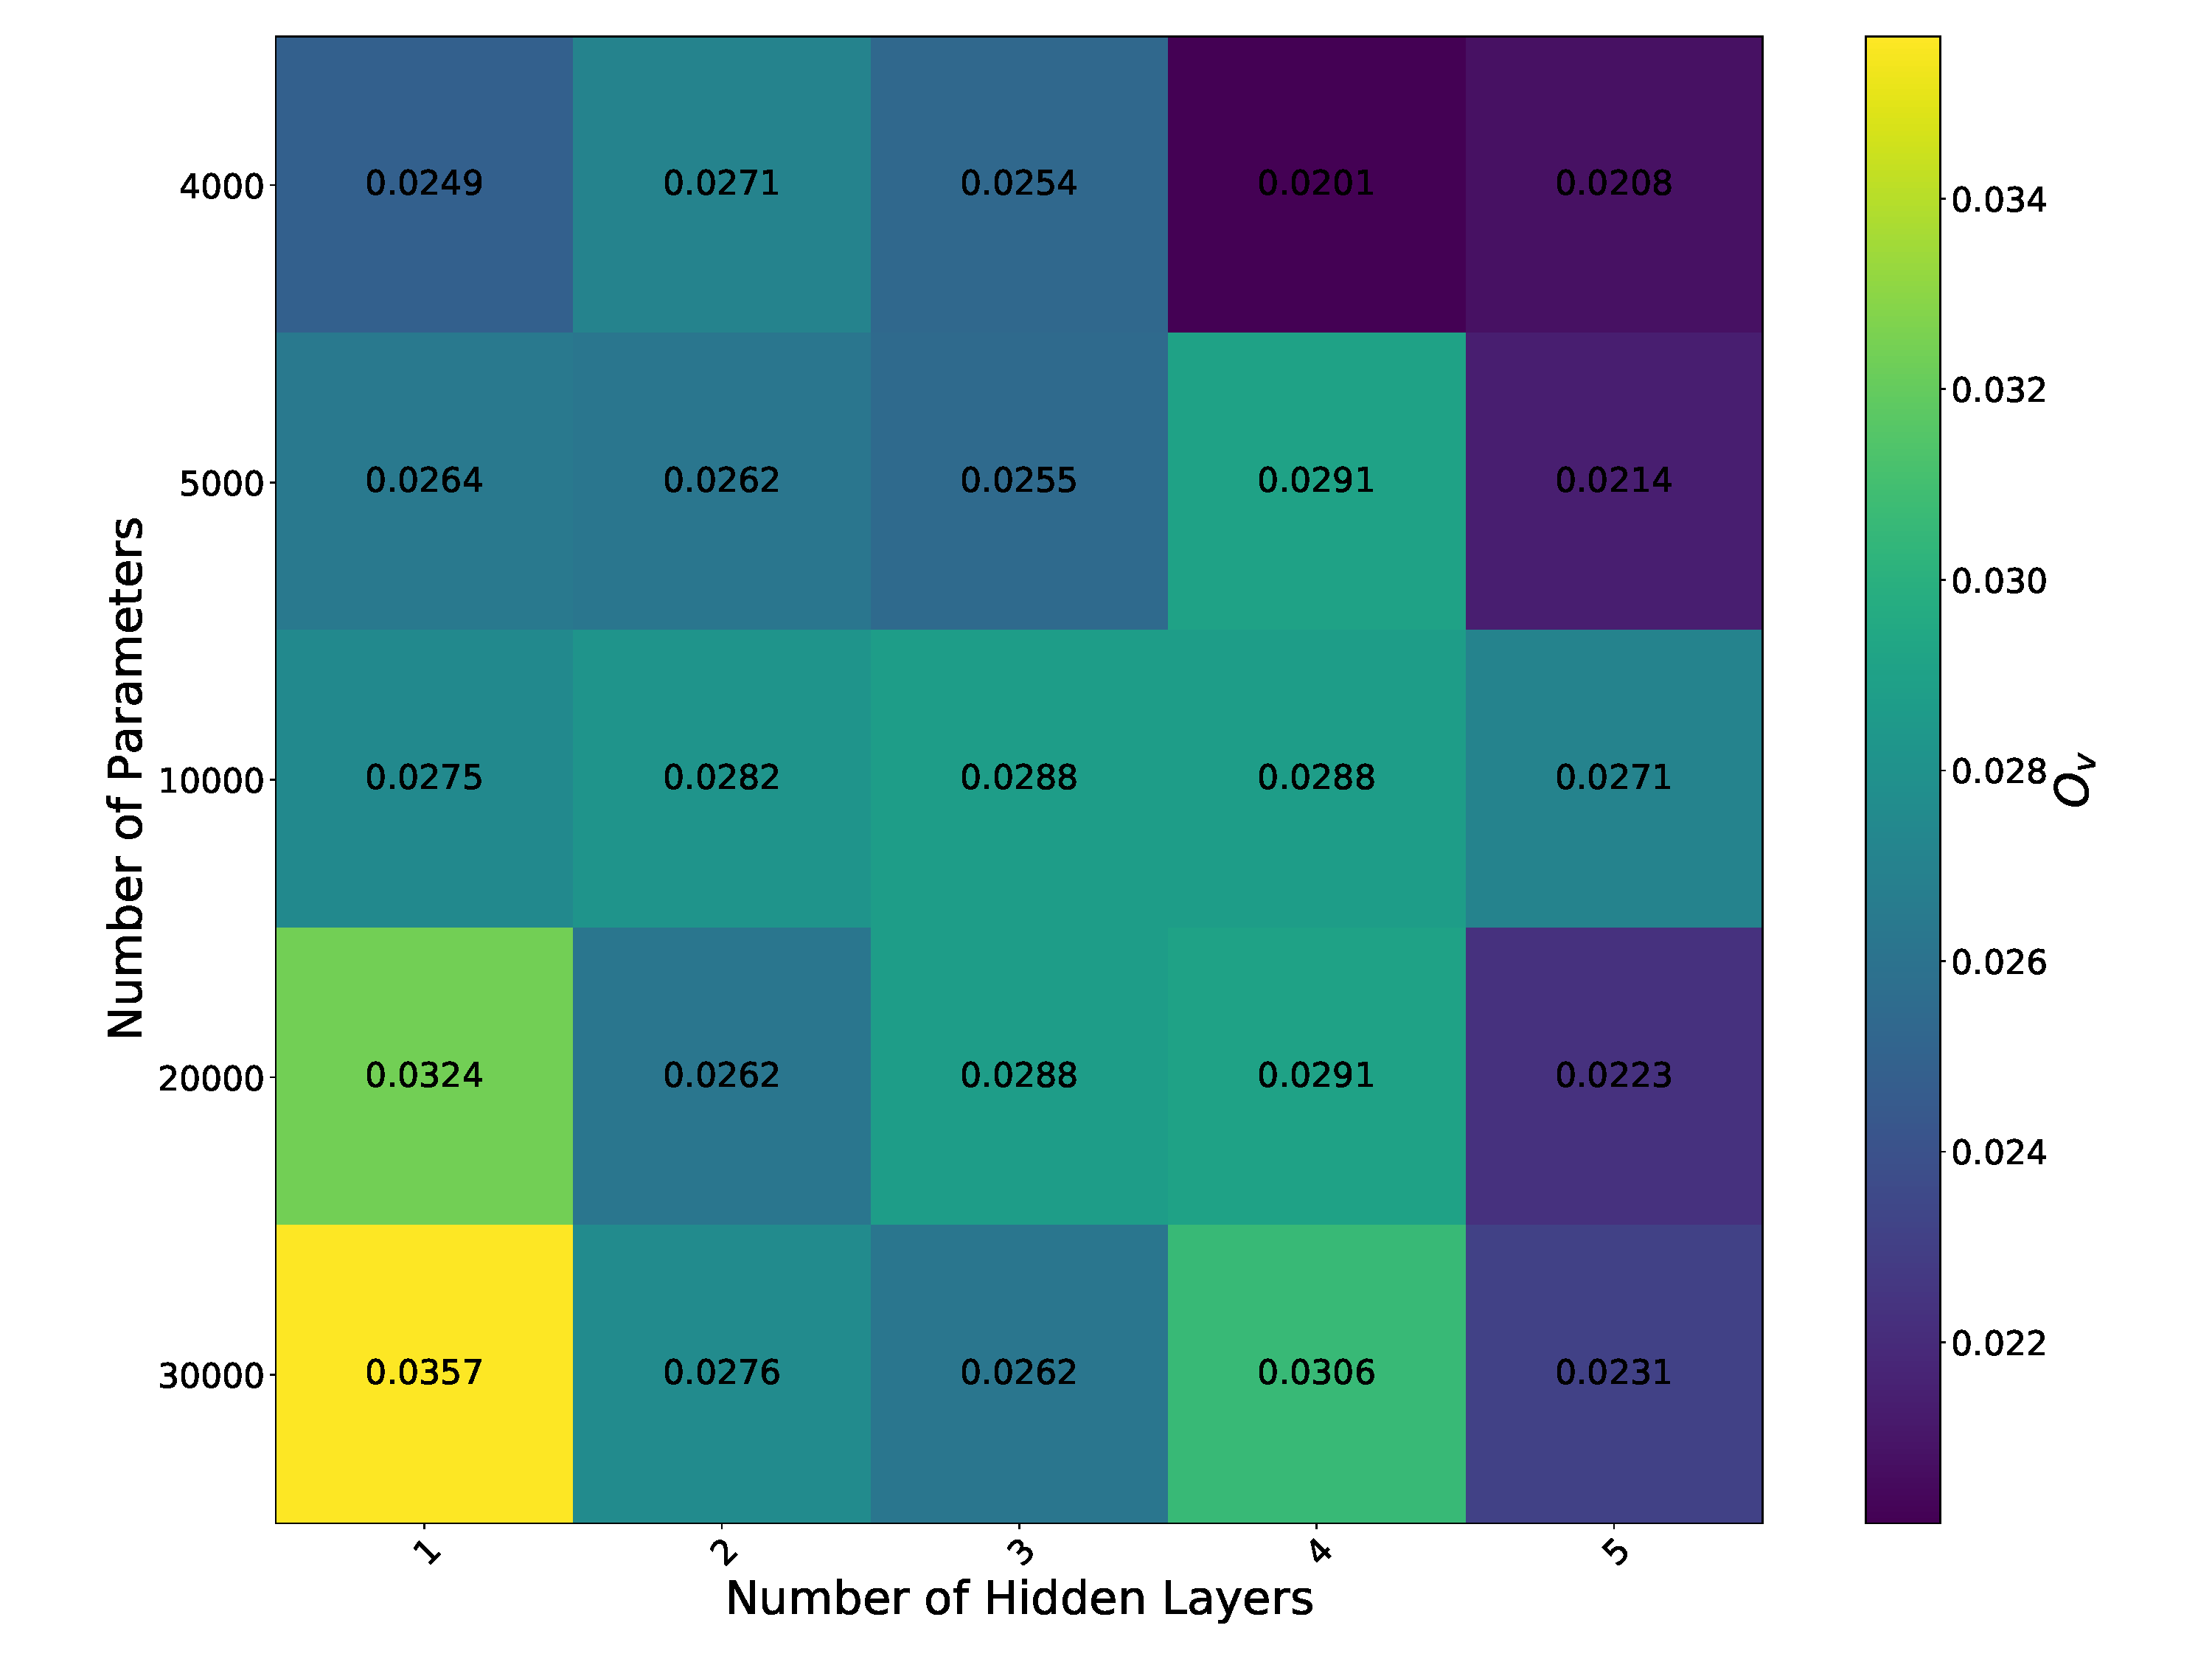
\includegraphics[width=\linewidth]{figs/FNN/Heat_ParaLayers}
\caption{The overtraining for FNNs of different sizes and depth, in the region where the observed AUCs are close to the best-performance obtained.}
\label{fig:RegionPara}
\end{figure}

\newpage

\paragraph{Weight Initialization and Activation Functions} \mbox{} \\

The Neural Networks architecture selected in the last sub-section is now selected to study the influence of activation functions and weight initialization on the AUC. As discussed in Section \ref{sec:optimization}, different weight initializations are designed to prevent the output of the activation functions from vanishing or exploding during the forward pass. Therefore, a high correlation between the two can be expected. \\
The effect of activation functions is studied by setting the activation function of all neurons in all hidden layers to either ReLU, leaky ReLU ($\alpha \in [0.1,0.3,0.5]$), ELU ($\alpha = 1$), or  SELU. For each activation function, different weight initializations namely Glorot, He, and Lecun with normal and uniform distributions are tested. The activation function of the output layer remains to be the Sigmoid function. The biases are initialized to zero. All other parameters are kept constant. \\

\begin{figure}[H]
\centering
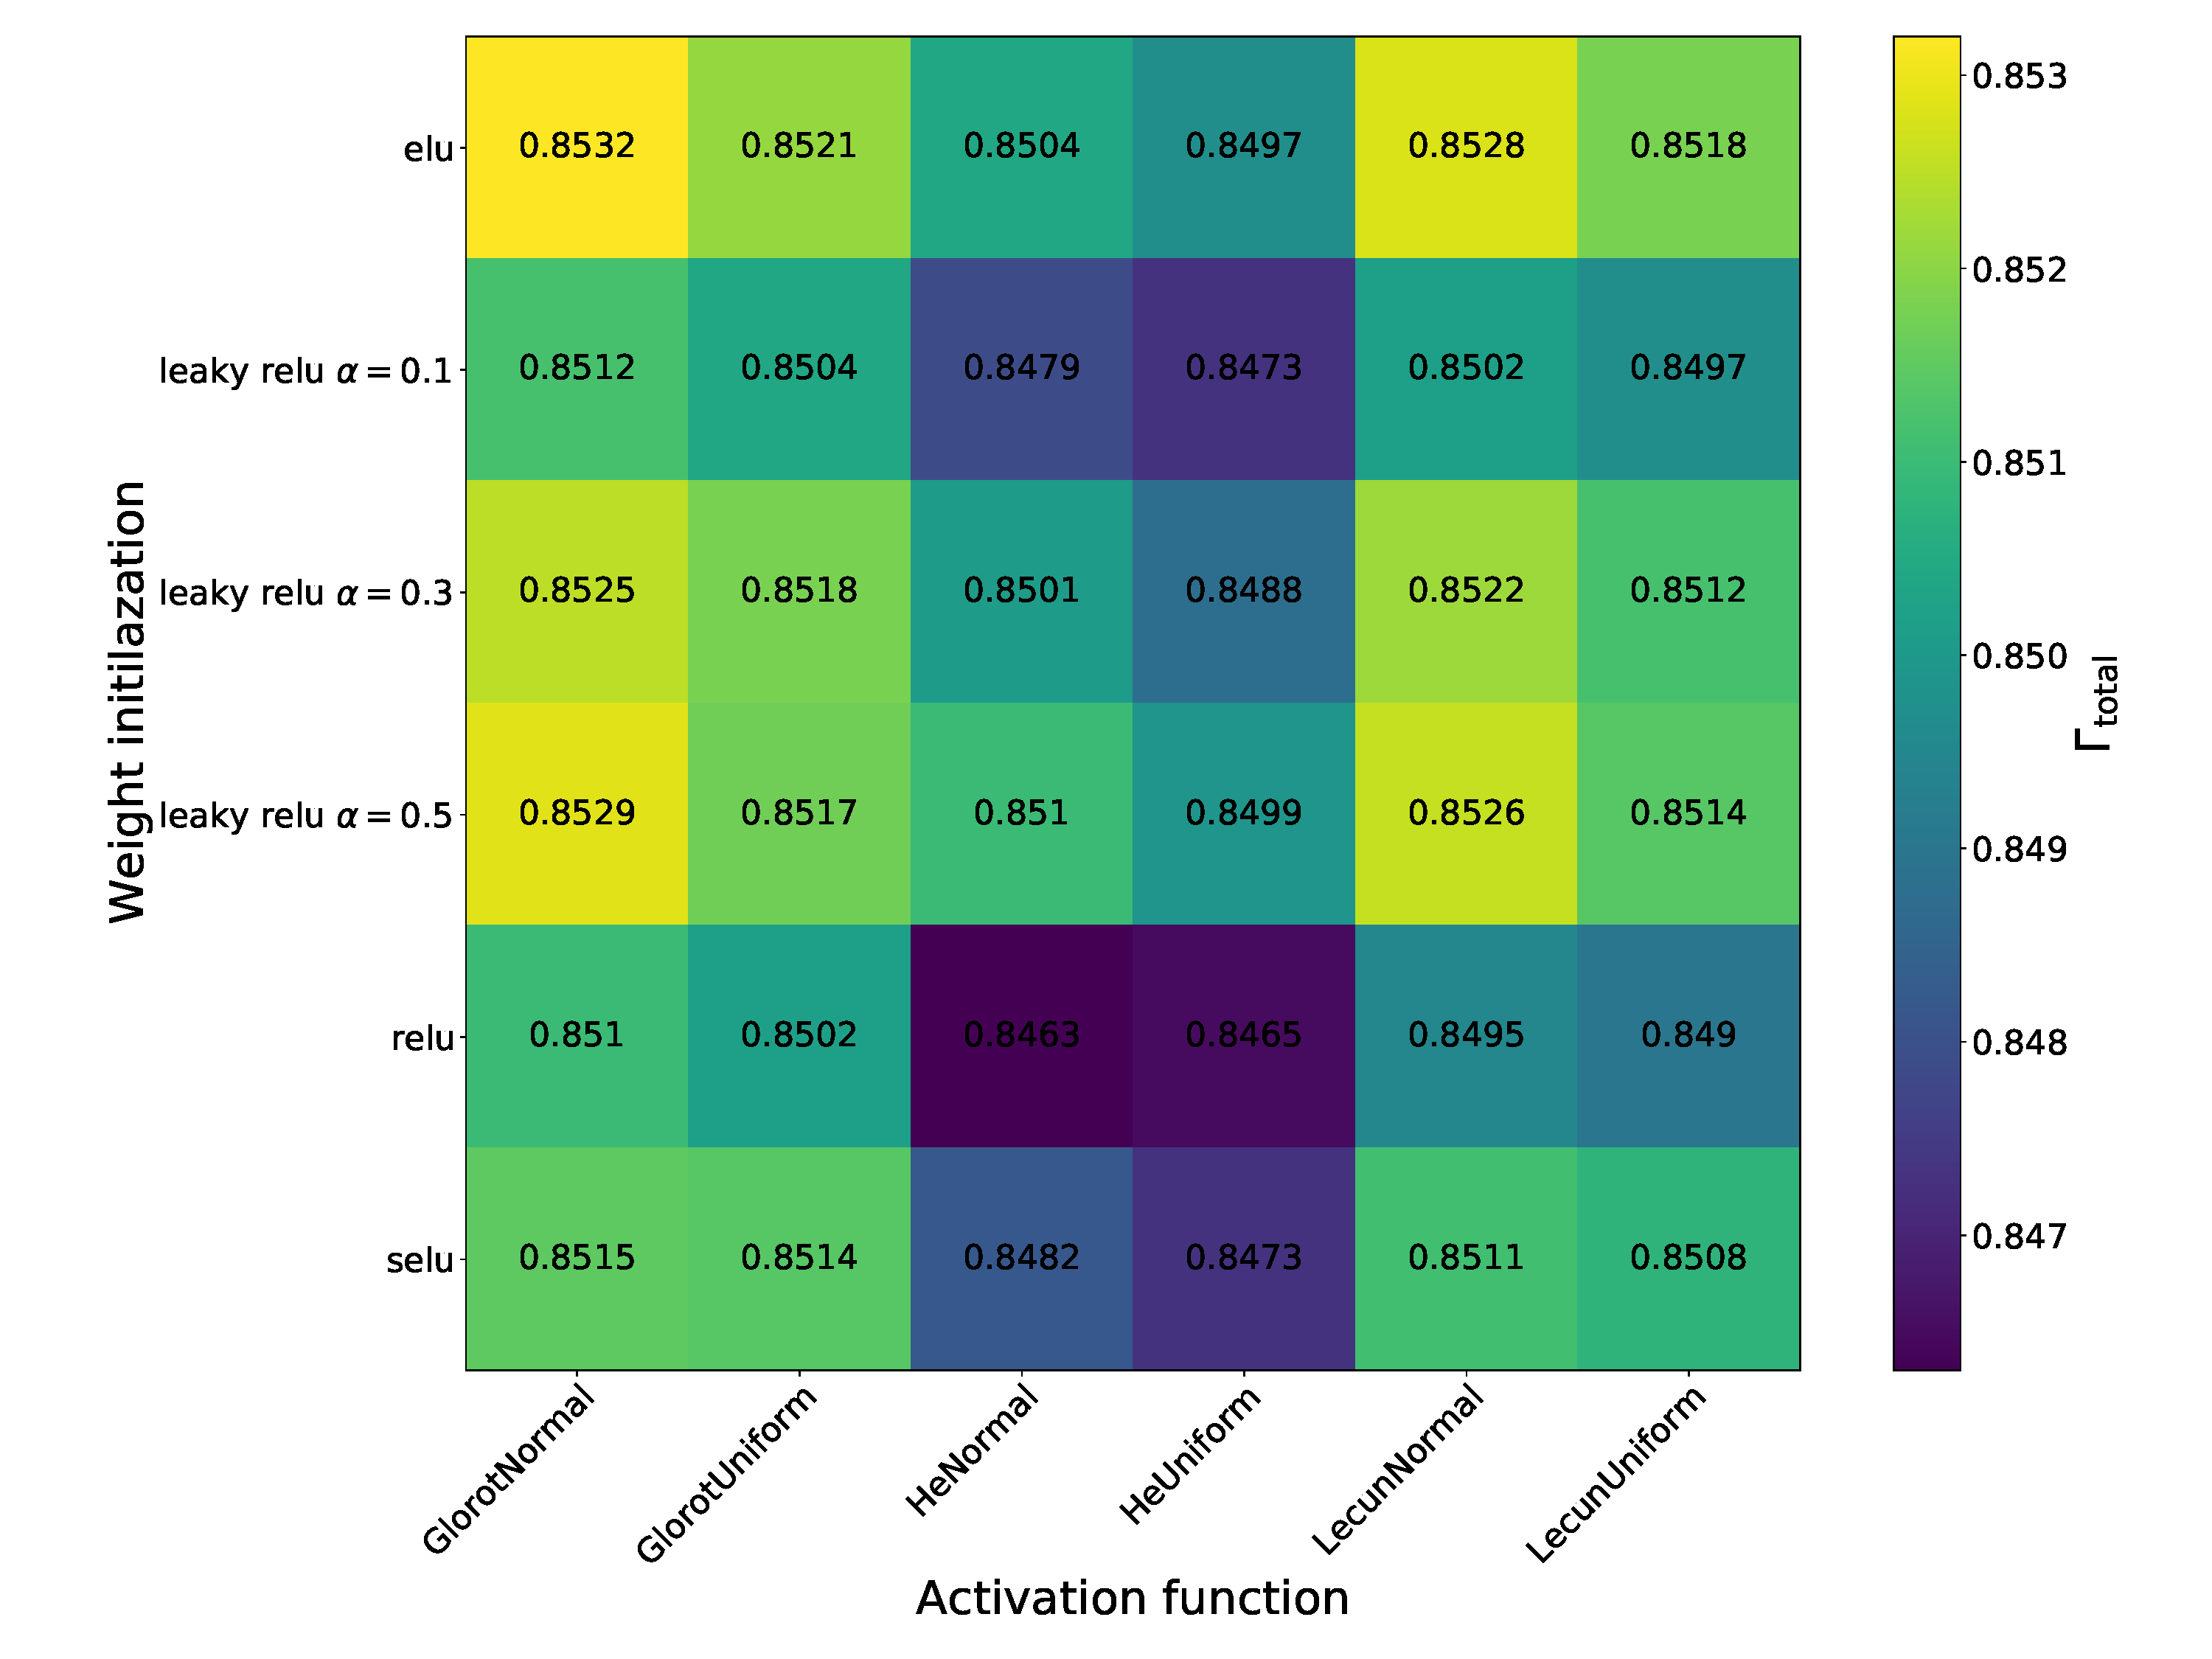
\includegraphics[width=\linewidth]{figs/FNN/Heat_Activ}
\caption{AUCs obtained for different choices of activation functions and weight initialization.}
\label{fig:HeatActiv}
\end{figure}

Figure \ref{fig:HeatActiv} shows the obtained AUCs for all combinations while Figure \ref{fig:OvActiv} shows the corresponding overtraining values. The best performance is reached when ELU is combined with the Glorot normal distribution weight initialization, which is the weight initialization that works best for all considered activation functions. The difference between normally and uniformly distributed weight initializations is minor but normally distributed initializations result in slightly higher AUC. \\
The ReLU activation function is outperformed for all considered by all other activation functions. This indicating that a training in which some weights are not updated, as is the case for ReLU, is not beneficial for this application. In fact, the performance increases with the slope constant $\alpha$ for leaky ReLU. In the case of ELU, a smooth transition between the output values for negative and positive net input results in the best $\Gamma_{\text{total}}$ for all weight initializations. The SELU activation function, specifically designed for FNNs, does not lead to an improved result compared to ELU. \\
The overtraining for all considered activation functions and weight initializations remains below 5\%. Counter-intuitively, the Neural Networks with the highest AUC also have the smallest overtraining and the lowest $\Gamma_{\text{total}}$ on the training dataset. Therefore, the additional performance gains come from the reduction of overtraining by the activation functions and weight initializations.

\begin{figure}[H]
\centering
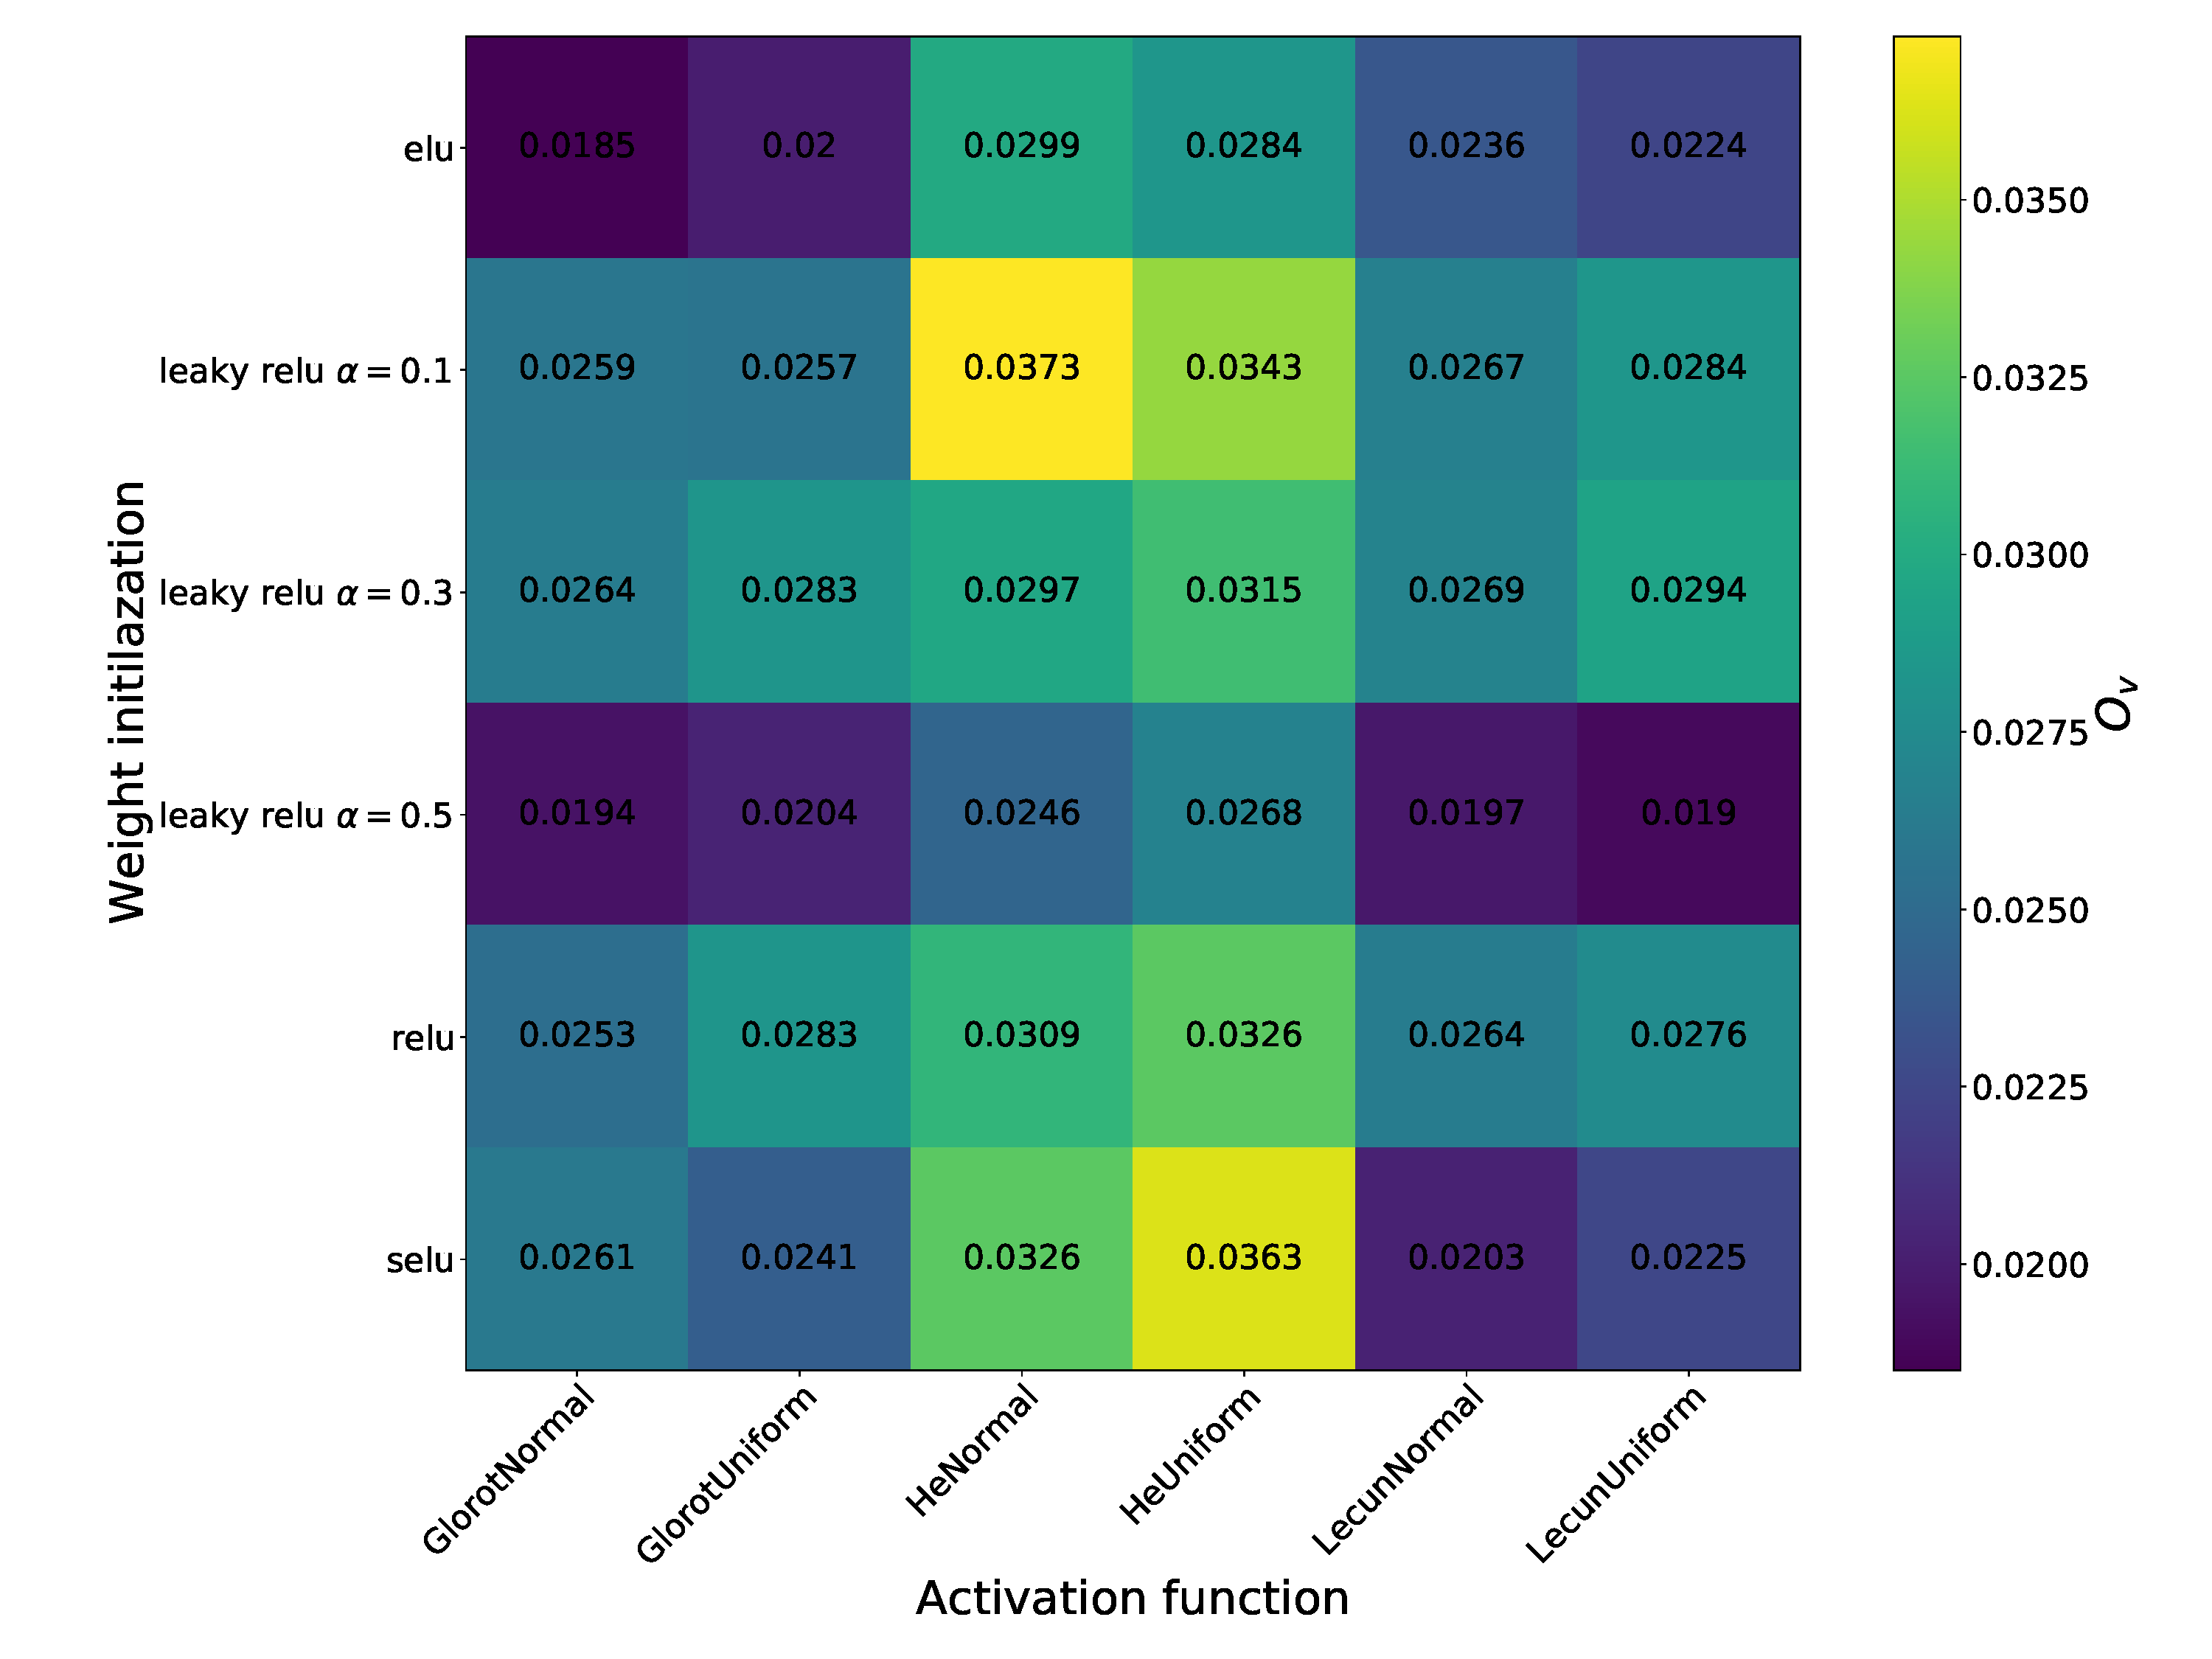
\includegraphics[width=\linewidth]{figs/FNN/Heat_Ovactiv}
\caption{The overtraining for different choices of activation functions and weight initialization.}
\label{fig:OvActiv}
\end{figure}

\newpage

\paragraph{Learning Rate and Optimization Algorithms}  \mbox{} \\

Building upon the results obtained in the first two studies, the performance for different optimization algorithms is investigated. The most impactful hyperparameters of the optimization algorithm are the learning rate, determining the step size of every weight update, and the batch size which is the number of events used during one iteration of the training. \\
Three different optimization algorithms are considered in this thesis: SGD, Adam, and Rmsprop. For each optimization algorithm, distinct learning rates are investigated together with varying the batch size. The different batch sizes are selected as powers of 2 and range from $2^8 = 256$ to $2^{14} = 16384$. All other ingredients of the Neural Network are kept constant. \\


\begin{figure}[H]
\centering
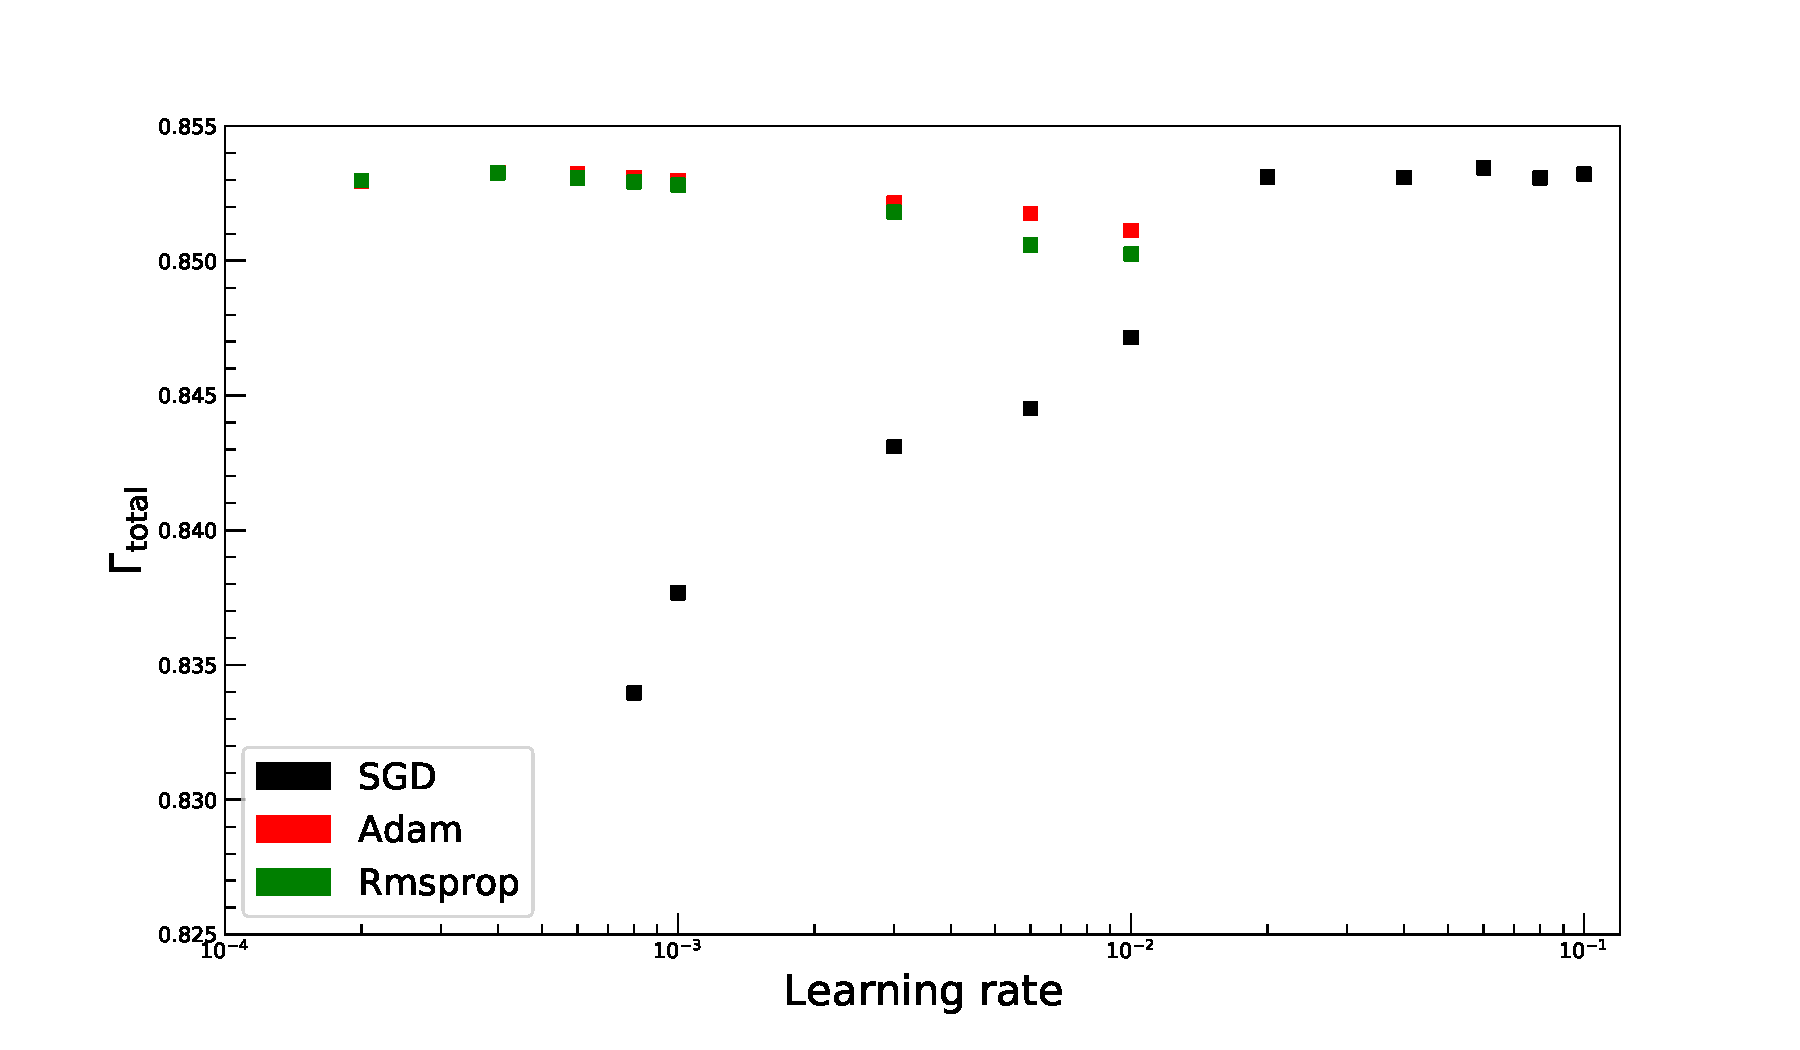
\includegraphics[width=\linewidth]{figs/FNN/LrAuc_All}
\caption{The obtained average AUC of FNNs with different learning rates and three distinct optimization algorithms.  The average includes the AUCs of the 3 best-performing Neural Networks with different batch sizes.}
\label{fig:LrAuc}
\end{figure}

Figure \ref{fig:LrAuc} shows the observed $\Gamma_{\text{total}}$ values for different learning rates and optimization algorithms while averaging over the 3 best-performing batch sizes for each learning rate. All three investigated optimization algorithms show a similar peak performance. The improvements gained by fine-tuning the learning rate within one order of magnitude are minor. For Adam and Rmsprop, even learning rates of one order of magnitude higher than the optimal observed learning rate result in only slightly worth AUCs while SGD is more sensitive. The reason being, Adam and Rmsprop calculate individually optimized learning rates for different parameters (weights and biases) based on the initial learning rate. On the other hand, SGD always applies the same learning rate for all parameters. This internal optimization is also reflected in the fact that Neural Networks trained with SGD tend to need more Epochs until the best AUC is reached, compared to Neural Networks trained with Rmsprop or Adam. All considered models have a similar overtraining for all considered learning rates, shown in Figure \ref{fig:OvLr}. The choice of the optimization algorithm used for training did not influence the overtraining. The Neural Networks with less than 1\% of overtraining are the models that have poor AUC, indicating that the training for these models did not converge. \\

\begin{figure}[H]
\centering
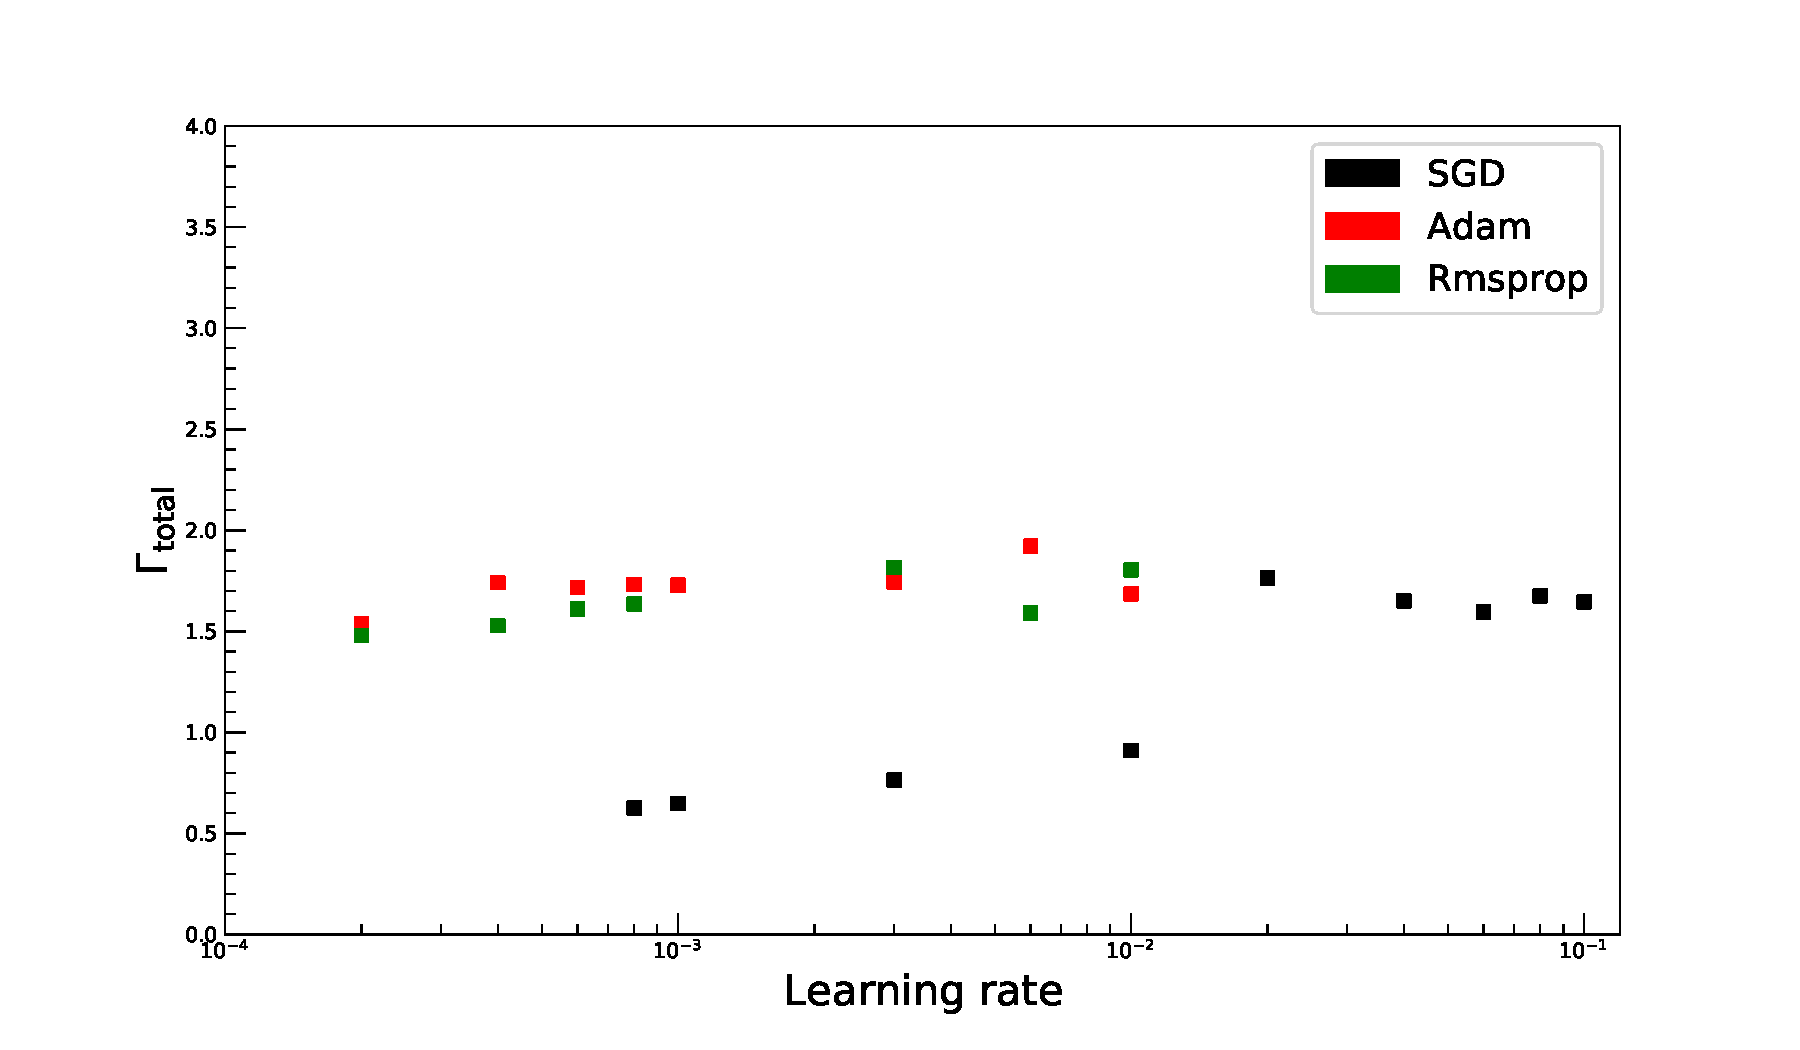
\includegraphics[width=\linewidth]{figs/FNN/LrOv_Fixed}
\caption{The overtraining of FNNs for different learning rates $Lr$ and three distinct optimization algorithms.}
\label{fig:OvLr}
\end{figure}

\begin{figure}[H]
\centering
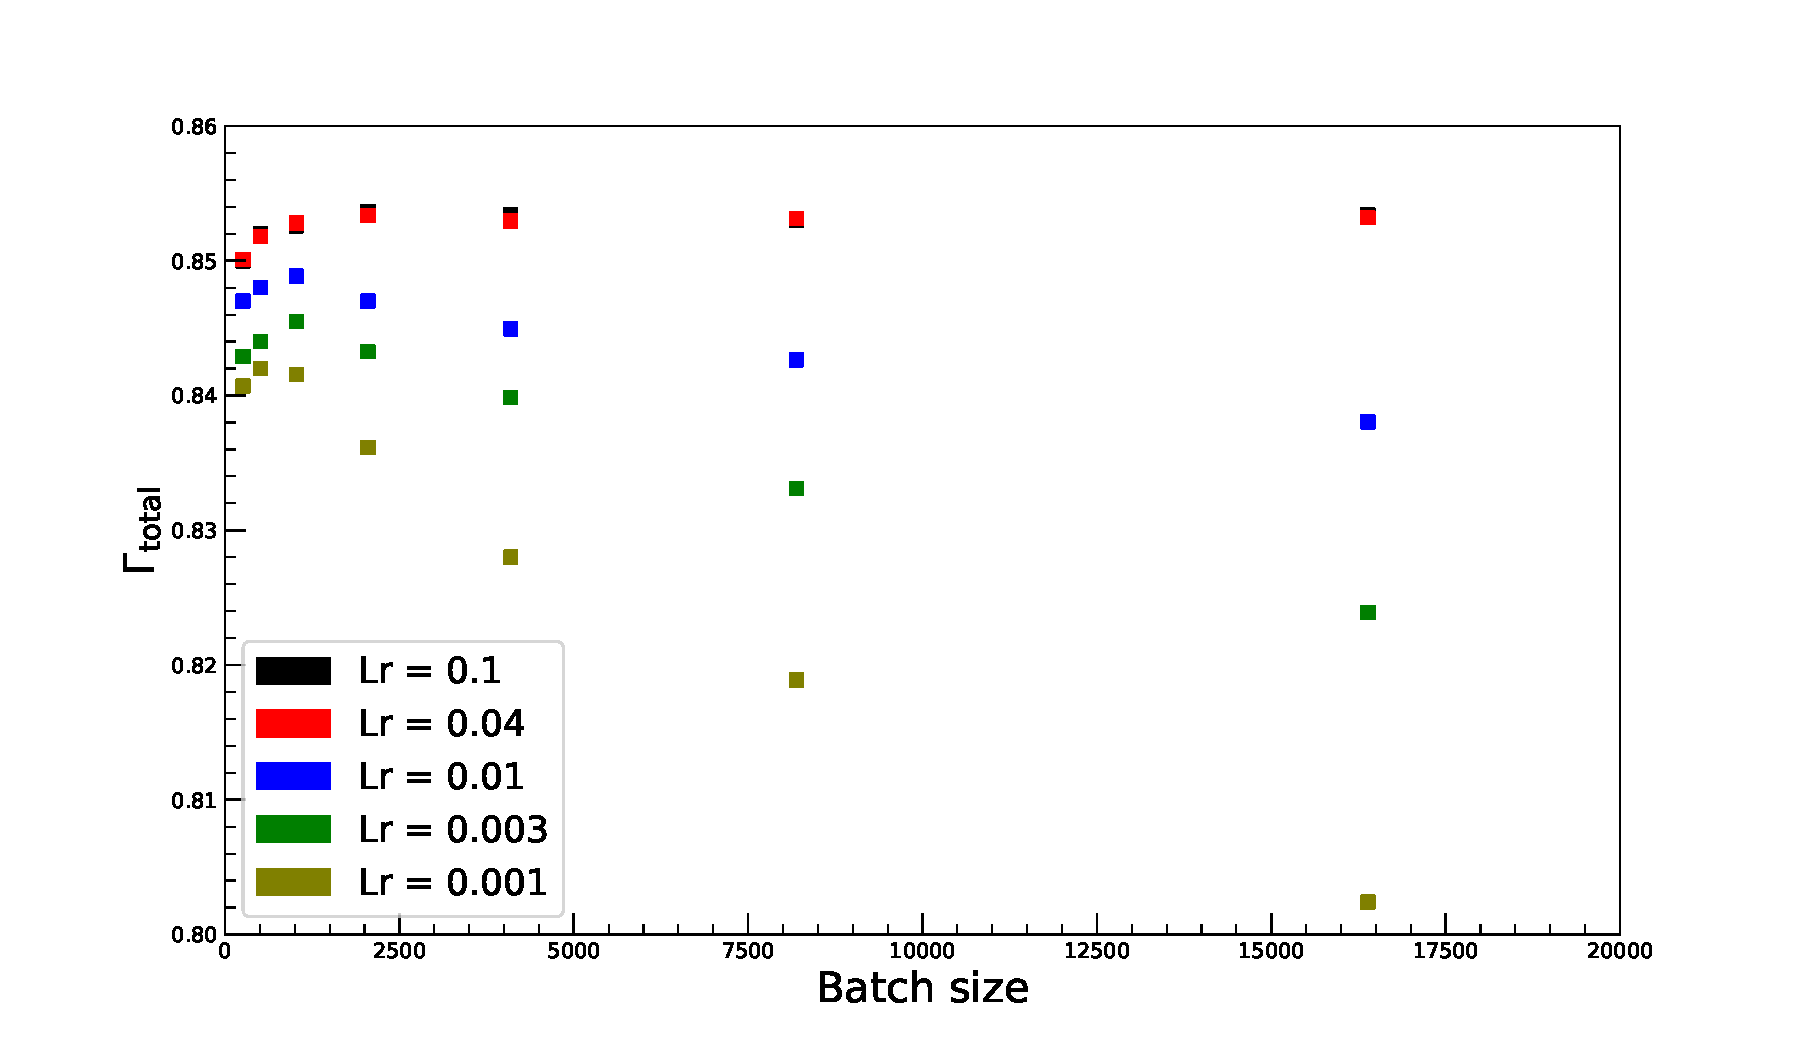
\includegraphics[width=\linewidth]{figs/FNN/BatchAuc_SGD}
\caption{The AUC as a function of the batch size and the learning rate. The Neural Networks are trained using SGD.}
\label{fig:SGDBatch}
\end{figure}

In order to study the dependence of $\Gamma_{\text{total}}$ on the batch size, Figure \ref{fig:SGDBatch} exclusively shows the results obtained by using SGD as the optimization algorithm. The AUC for learning rates close to the optimal observed choice (black and red) is almost independent of the batch size. On the other hand, for smaller learning rates, the batch size has a significant impact. This is because, for those Neural Networks the maximum considered number of 120 Epochs is reached which in turn is a direct consequence of the small batch size. Neural Networks trained with small batch sizes perform less weight updates per Epoch. When the maximum number of Epochs is not sufficiently high, the small number of weight updates leads to a non-optimal weight configuration that decreases the obtained AUC. The drop in peak performance for small batch sizes ($< 2000$) can be attributed to the fact that a small batch may not contain events from all backgrounds. The weight updates calculated based on this batch may not be accurate enough to lead to the optimal weight configuration during training. \\
The best Neural Network obtained uses Adam with a learning rate of 0.003 and a batch size of 2048.  The maximum  $\Gamma_{\text{total}}$ reached is 0.853, with an overtraining of 0.016 on the testing set.




\paragraph{Polynomial Learning Rate Decay} \mbox{} \\
 

\begin{figure}[H]
\begin{subfigure}{.33\textwidth}
  \centering
  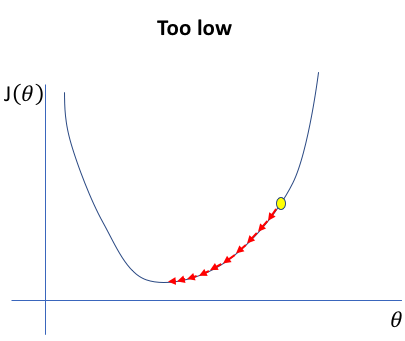
\includegraphics[width=.99\linewidth]{figs/TooLow}
  \caption{}
  \label{fig:TooLow}
\end{subfigure}%
\begin{subfigure}{.33\textwidth}
  \centering
  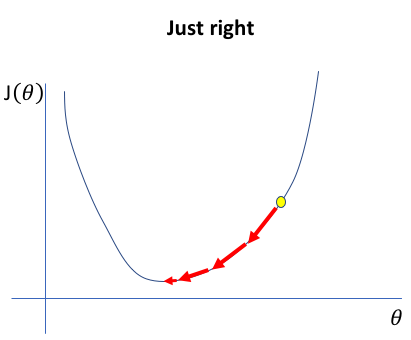
\includegraphics[width=.99\linewidth]{figs/JustRight}
  \caption{}
  \label{fig:JustRight}
\end{subfigure}
\begin{subfigure}{.33\textwidth}
  \centering
  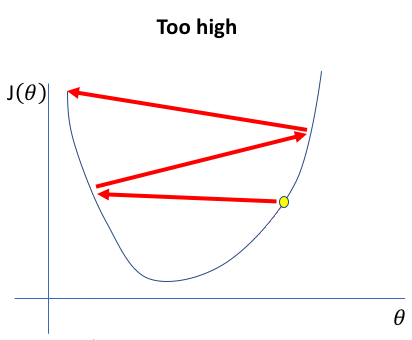
\includegraphics[width=.99\linewidth]{figs/TooHigh}
  \caption{}
  \label{fig:TooHigh}
\end{subfigure}%
\caption{Training of a Neural Network trained with a too low (a), a too high and a polynomial decaying learning rate. \cite{lrdecay} }
\label{fig:PolyTrain}
\end{figure}


Three different trainings scenarios for the same problem are shown in Figure \ref{fig:PolyTrain}. In the first case (\ref{fig:TooLow}), the learning rate is too low to reach the minimum of the Loss functions $J(\theta)$ during the training. On the other hand, if the learning rate is too large (\ref{fig:TooHigh}), the weight updates overshoot the point of best performance, resulting in a decreased AUC. Both cases can be avoided when using polynomial learning rate decay (\ref{fig:JustRight}). In polynomial learning rate decay, the initial learning rate $Lr_{\text{int}}$ is adjusted for each Epoch according to
\begin{equation}
Lr(E) = Lr_{\text{int}} \cdot (1-\frac{E}{E_{\text{tot}}})^{n}
\end{equation}
where $Lr(E)$ is the learning rate at Epoch $E$, and $n$ is the used polynomial power. For this technique, the total number of Epochs $E_{\text{total}}$ has to be fixed. Using polynomial learning rate decay results in a more smooth coverage of the training towards the minimum. \\
For the studies on polynomial learning rate decay in this thesis, SGD was selected as the optimization algorithm to investigate the gained improvements independently of the parameter-by-parameter optimization used by Adam and Rmsprop. The initial learning is varied between 0.02 and 0.3, building upon the knowledge gained in the previous sub-section. Considered polynomials have the power of 1 to 3. The other parameters of the Neural Network are kept constant. \\

\begin{figure}[H]
\centering
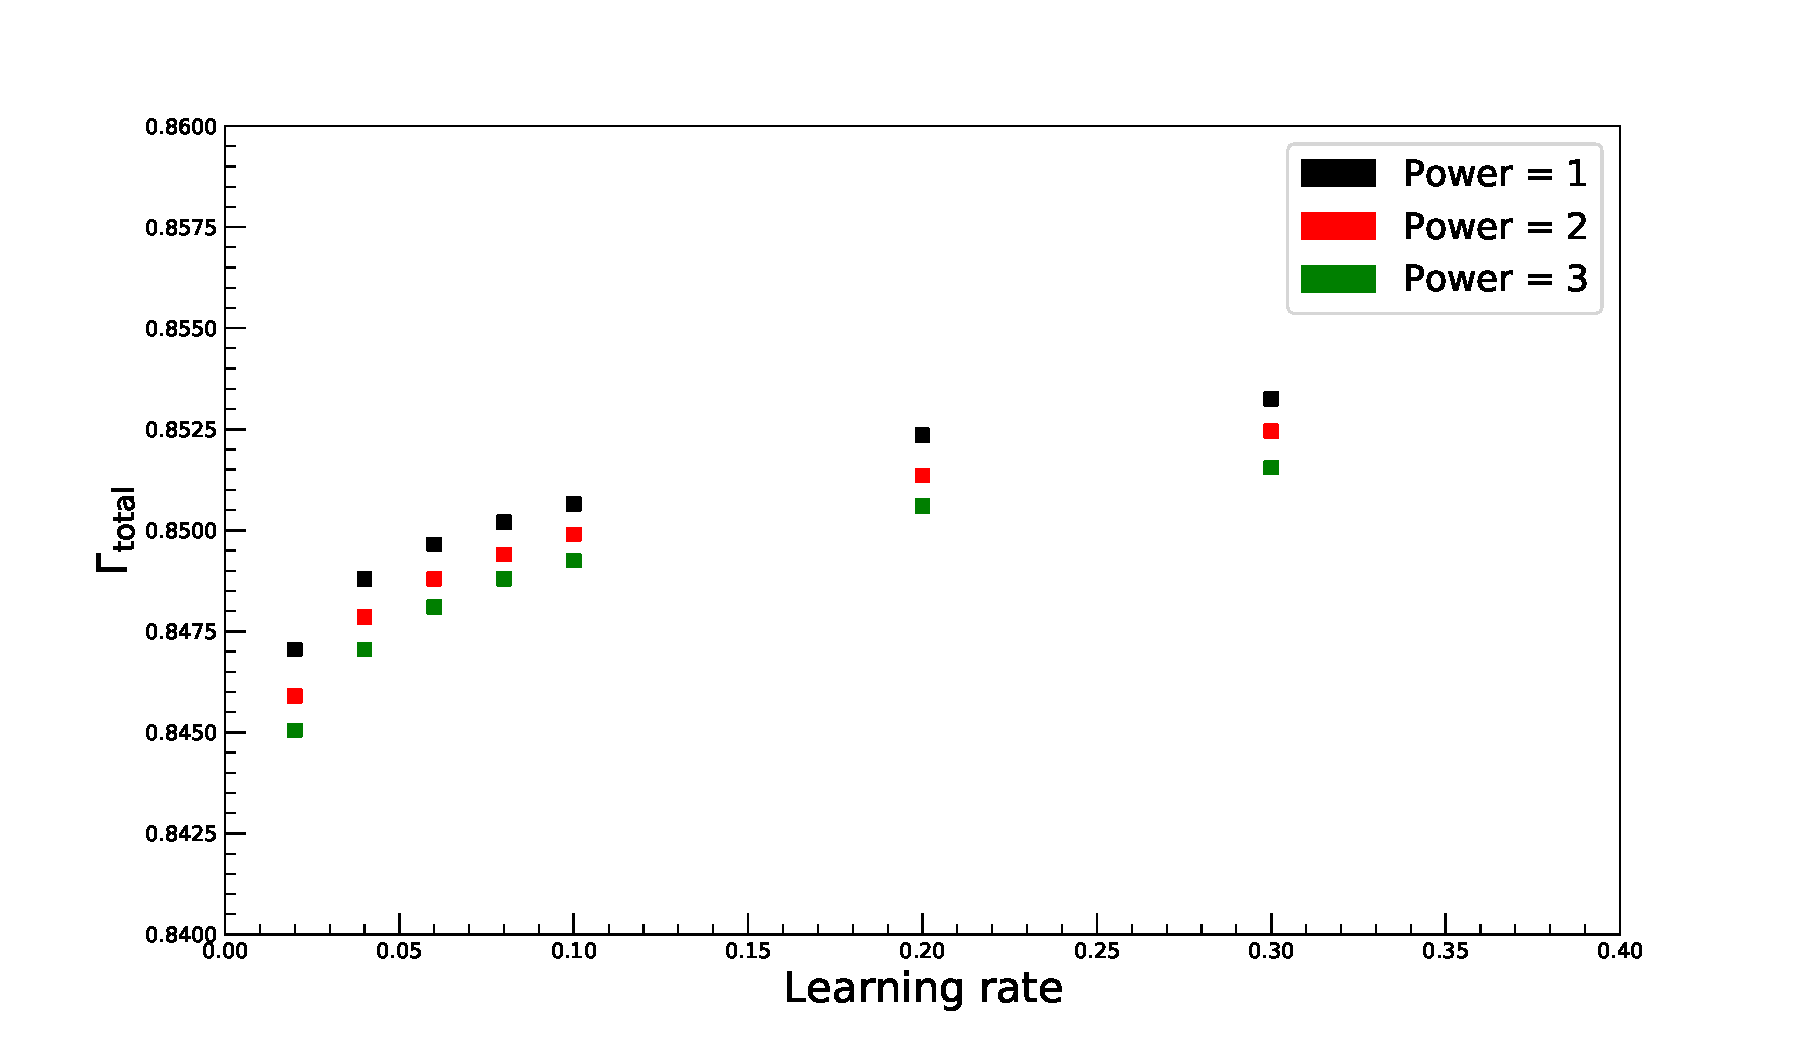
\includegraphics[width=0.93\linewidth]{figs/FNN/PolyAuc}
\caption{Obtained AUCs for FNNs trained using polynomial learning rate decay.}
\label{fig:PolyAuc}
\end{figure}

Figure \ref{fig:PolyAuc} shows the results of the polynomial learning rate decay.
Within the considered hyperparameter ranges, no improvement of the peak performance is observed compared to the training with fixed learning rates. Learning rate decays with polynomials of power 1 perform best among all investigated learning rates. The reason for this is not apparent and needs further investigations in the future. One drawback of polynomial learning rate decay is that Neural Networks, on average, have to be trained longer until the Epoch with the best performance is reached. However, for all learning rates considered with the exception of $Lr_{\text{int}} = 0.02$ the Epoch having the best performance is more than 5 Epochs away from $E_{\text{tot}} = 80$. The overall stability of the best AUC against different learning rates is only improved slightly (cf. Figure \ref{fig:LrAuc}). \\

\begin{figure}[H]
\centering
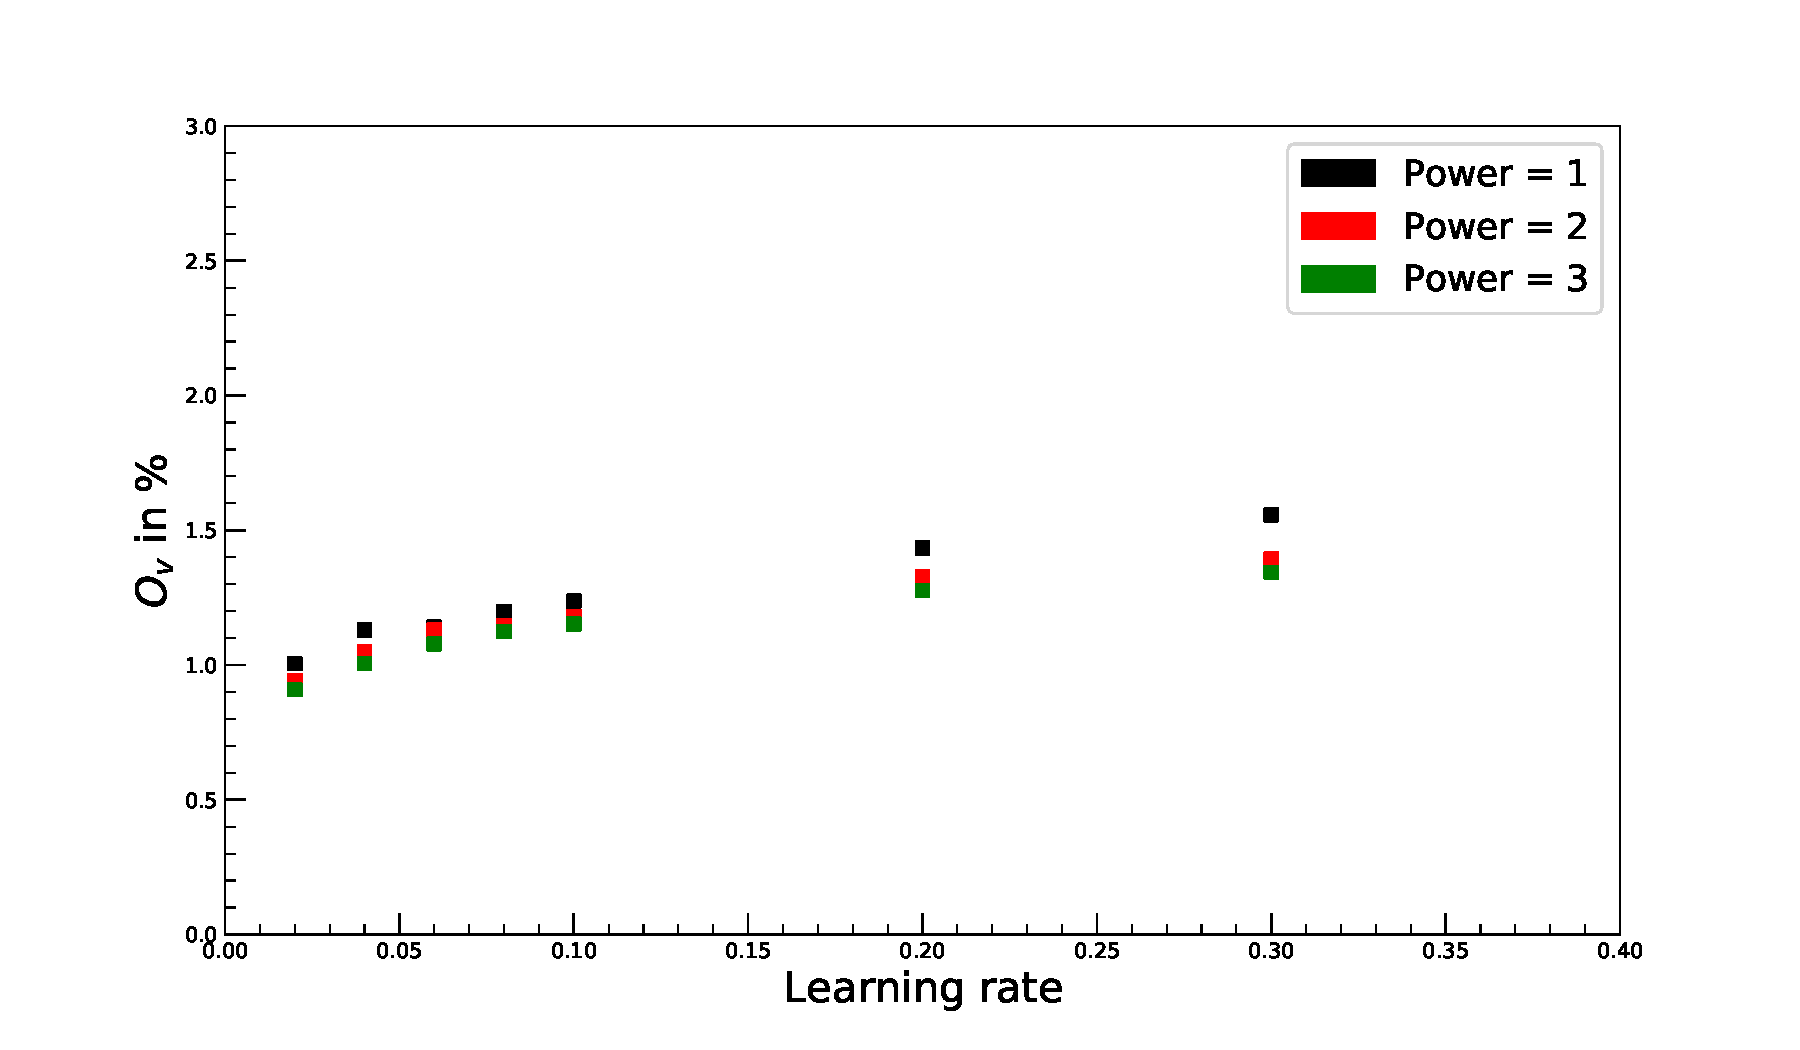
\includegraphics[width=0.93\linewidth]{figs/FNN/PolyOv}
\caption{The overtraining for FNNs trained using polynomial learning rate decay.}
\label{fig:PolyOv}
\end{figure}

The overtraining of the Neural Networks trained with polynomial learning rate decay, shown in Figure \ref{fig:PolyOv}, decreases with the learning rate and is independent of the power of the polynomial used. Similar to the overtraining observed for SGD using a fixed learning rate, all trained models have an overtraining below 1.5\%.




\paragraph{Cyclic Learning Rate Decay} \mbox{} \\

\begin{figure}[H]
\begin{subfigure}{.5\textwidth}
  \centering
  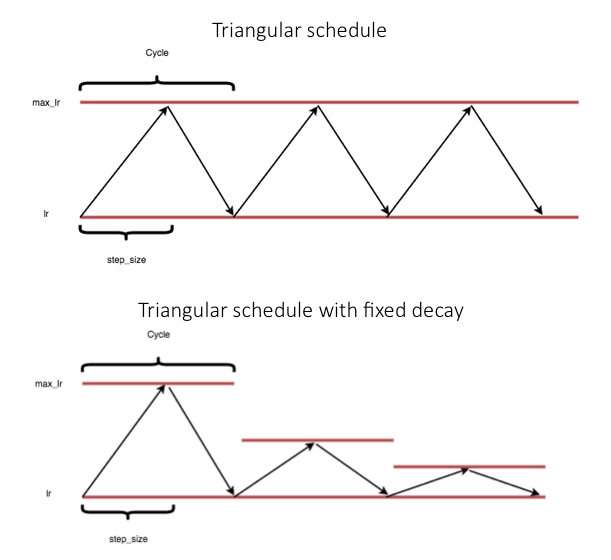
\includegraphics[width=.95\linewidth]{figs/Cycle}
  \caption{}
\end{subfigure}%
\begin{subfigure}{.5\textwidth}
  \centering
  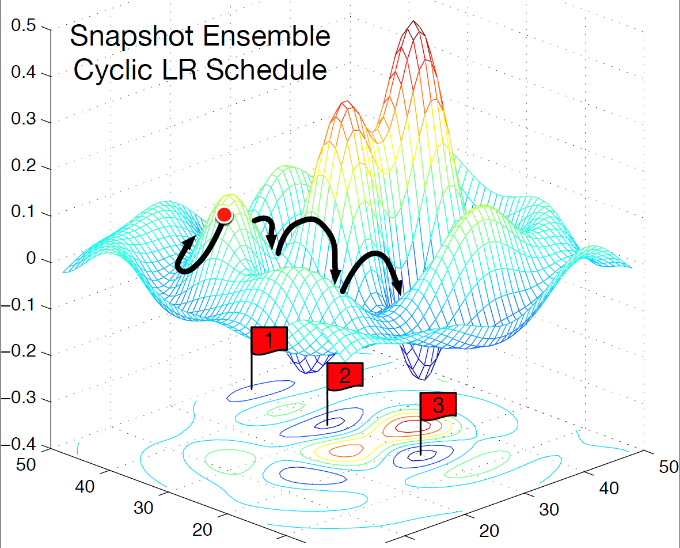
\includegraphics[width=.97\linewidth]{figs/topolgy}
  \caption{}
\end{subfigure}
\caption{a) The learning rate schedule for cyclic learning rate decay with and without additional decay of the maximum learning rate ``max\_ lr''. b) The topology of a Loss function for which cyclic learning rate decay can improve the performance of a Neural Network. The flags 1, 2 indicate the position of local minima where as flag 3 indicates the position of the global maximum. \cite{cyl1,cyl2}}
\label{fig:CylicTrain}
\end{figure}

Another attempt to improve the AUC by varying the learning rate during training is cyclic learning rate decay. The functionality is illustrated in Figure \ref{fig:CylicTrain}; during one cycle, the learning rate is linearly increased from a predefined minimum learning rate to a predefined maximum learning rate and after that linearly decreased until the minimum learning rate is reached. The number of batches needed to move from the maximum to the minimum learning rate or the other way around, is a tunable hyperparameter called \textit{stepsize}. Moreover, the maximum learning rate can be decreased after every cycle. This learning rate schedule is designed to prevent the training from getting stuck in a local minima or on a saddle points. \\
The cyclic learning rate decay study conducted 3 different parameters. The maximum learning rates considered are of the magnitude $10^{-1}$, while the minimum learning rates are of the magnitude $10^{-2}$. Simultaneously 5 different stepsizes are considered, which are chosen close to the suggested $2-8$ iterations per Epoch ($\sim 160 - 640$) in \cite{stepsize}. Each combination is trained with a static maximum learning rate and a maximum learning rate that decreased to its half value after each cycle. All other parameters are the same parameters used for the previous learning rate study. \\

\begin{figure}[H]
\centering
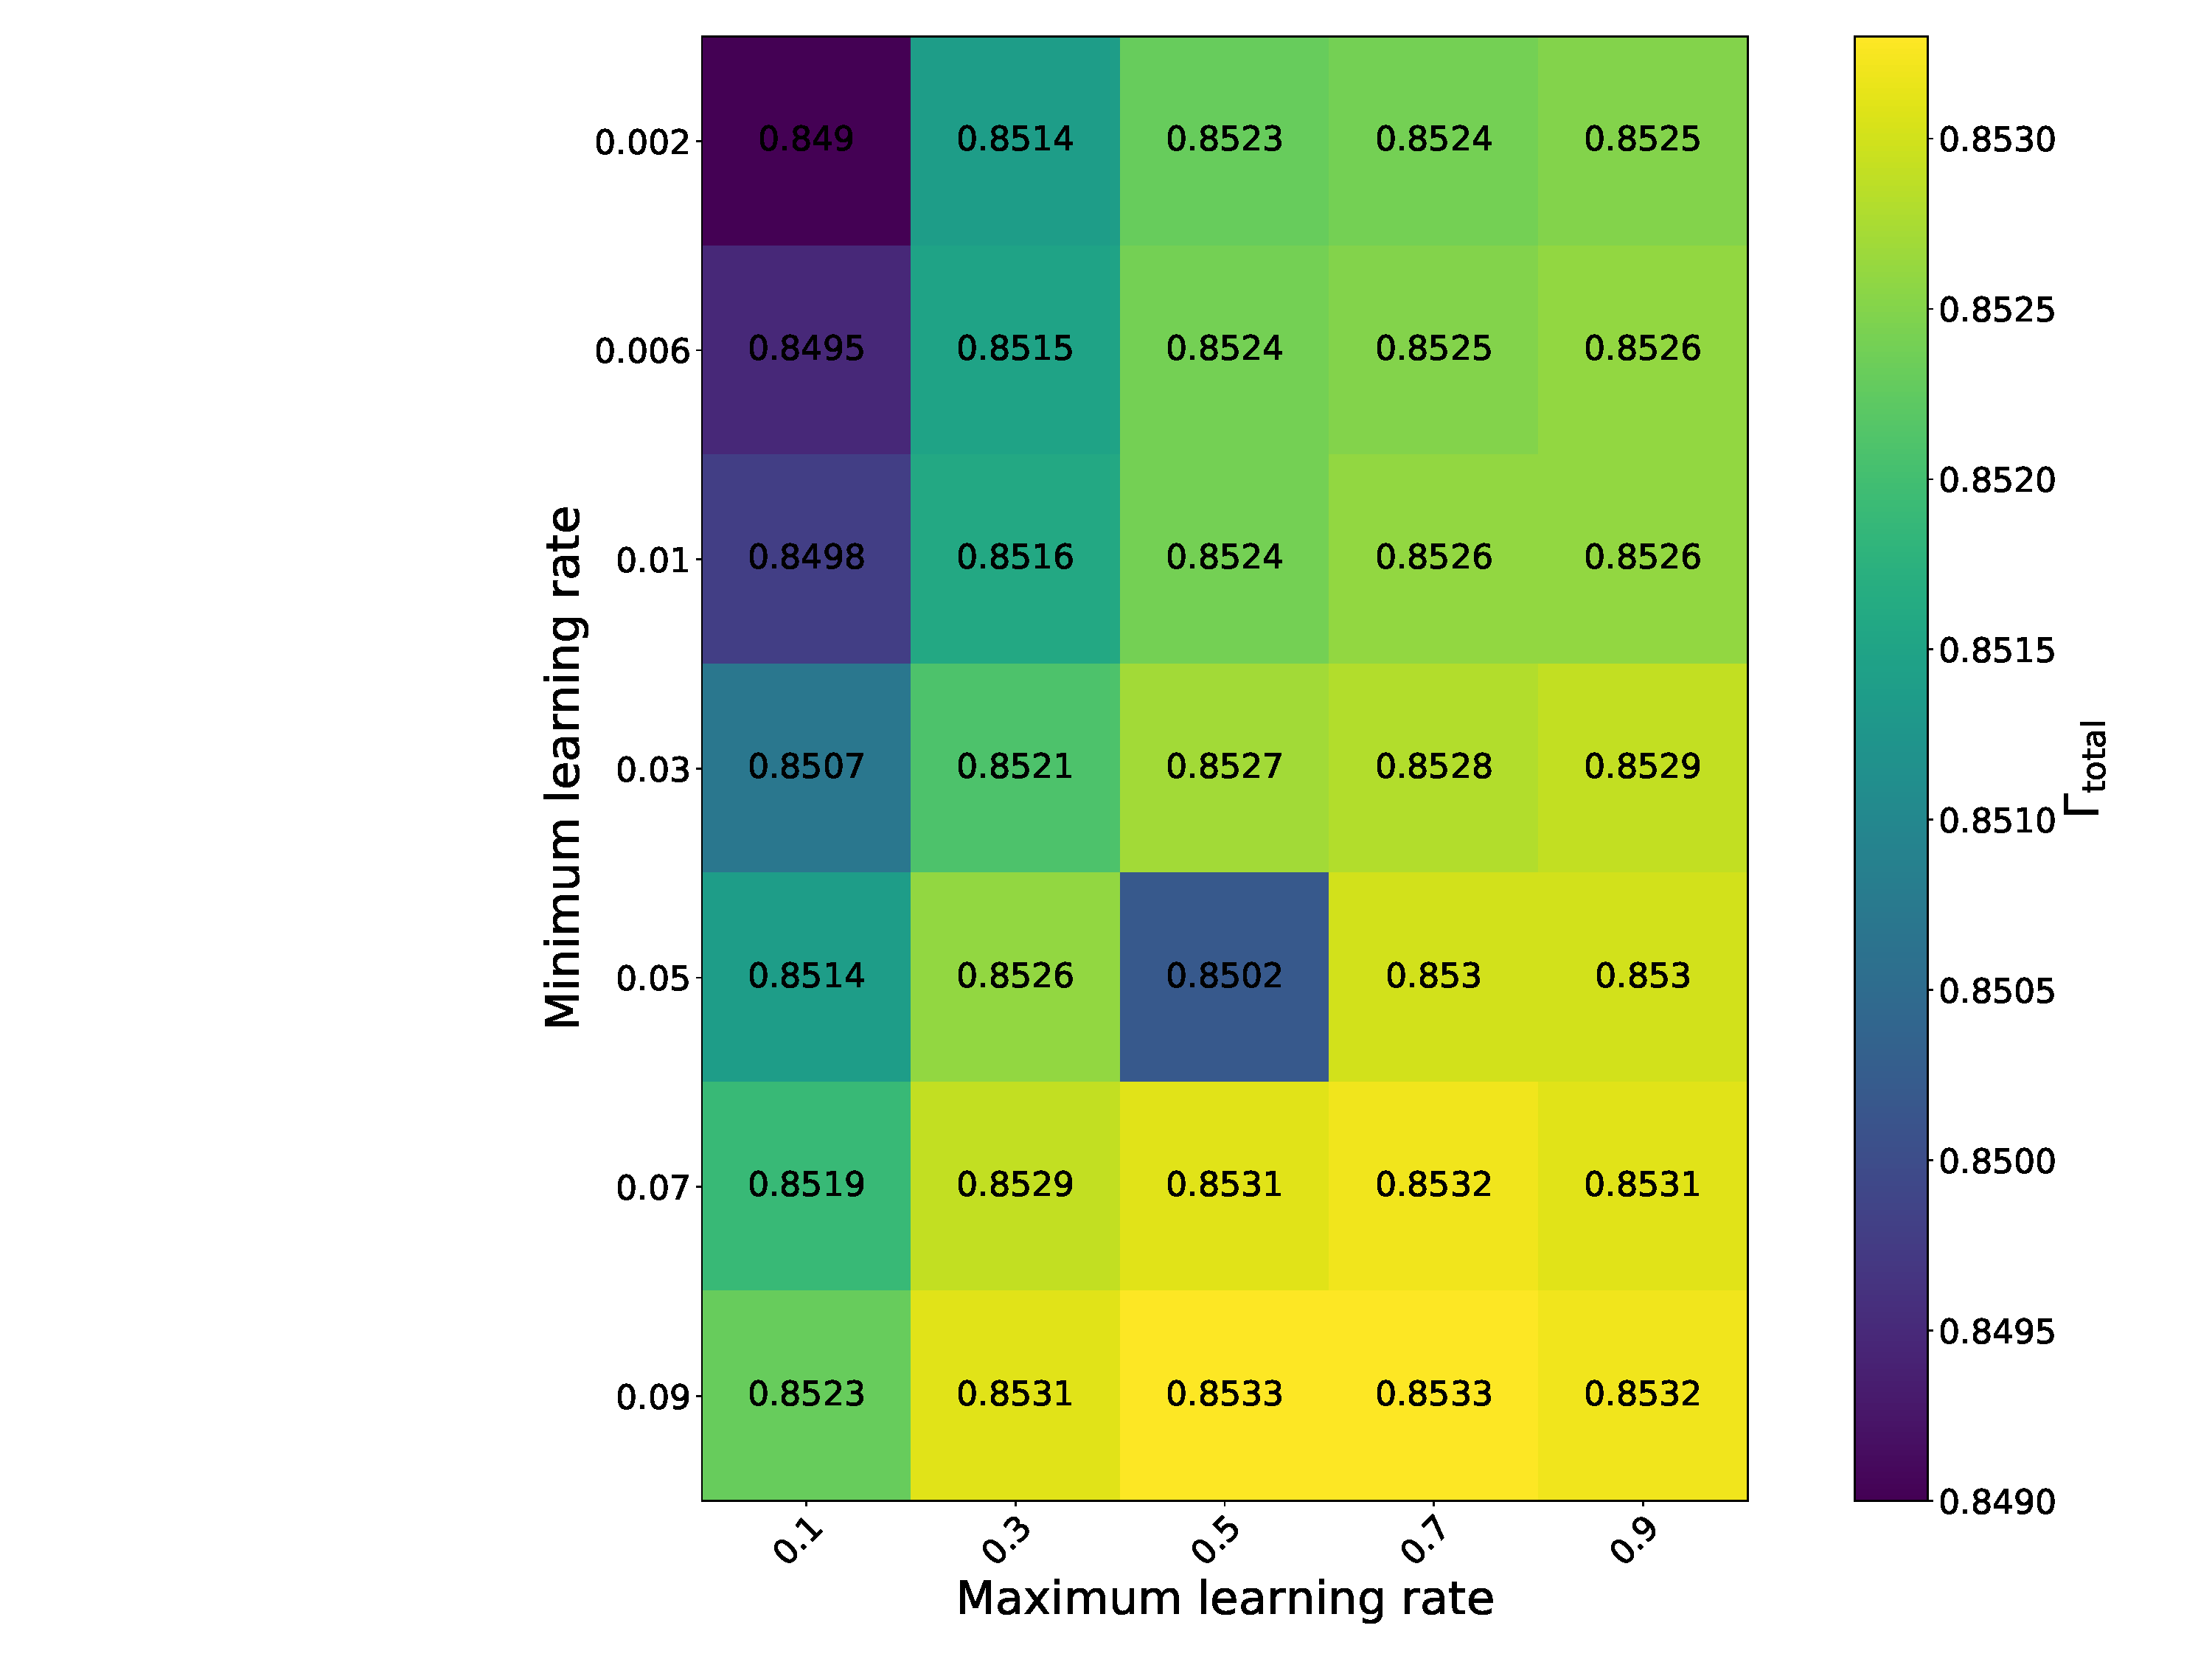
\includegraphics[width=\linewidth]{figs/FNN/Heat_MinMax}
\caption{The dependence between the maximum and the minimum learning rates of FNNs trained with cyclic learning rate decay.}
\label{fig:CylicHeatLr}
\end{figure}

\vspace{-0.1cm}

The heatmap in Figure \ref{fig:CylicHeatLr} shows the results obtained for the different combinations of minimum and maximum learning rates where the quoted $\Gamma_{\text{total}}$ values are the average AUC over all stepsizes for both the fixed and the decaying maximum learning rate training. Varying the minimum learning rate improves the performance of the Neural Networks more than varying the maximum learning rate. Therefore, no second minimum that results in a better performance is found. The drop in performance obtained for models trained with a maximum learning rate of 0.1 is most likely not an indication for a local minimum but rather due to the fact that the training did not converge during 120 Epochs. For minimum learning smaller than 0.3, the same problem occurred.  Similar to polynomial learning rate decay, Neural Networks trained with cyclic learning rate decay need more Epochs to until the best performance is found compared to Neural Networks trained with a fixed learning rate. \\
The comparison between cyclic learning rate decay with fixed maximum learning rate and with additional decay of the maximum learning rate is shown in Figure \ref{fig:CylicLr} where only the 5 best-performing Neural Networks were considered for each learning rate. No significant difference between the two learning schedules (red and black squares) is observable. \\

\begin{figure}[H]
\centering
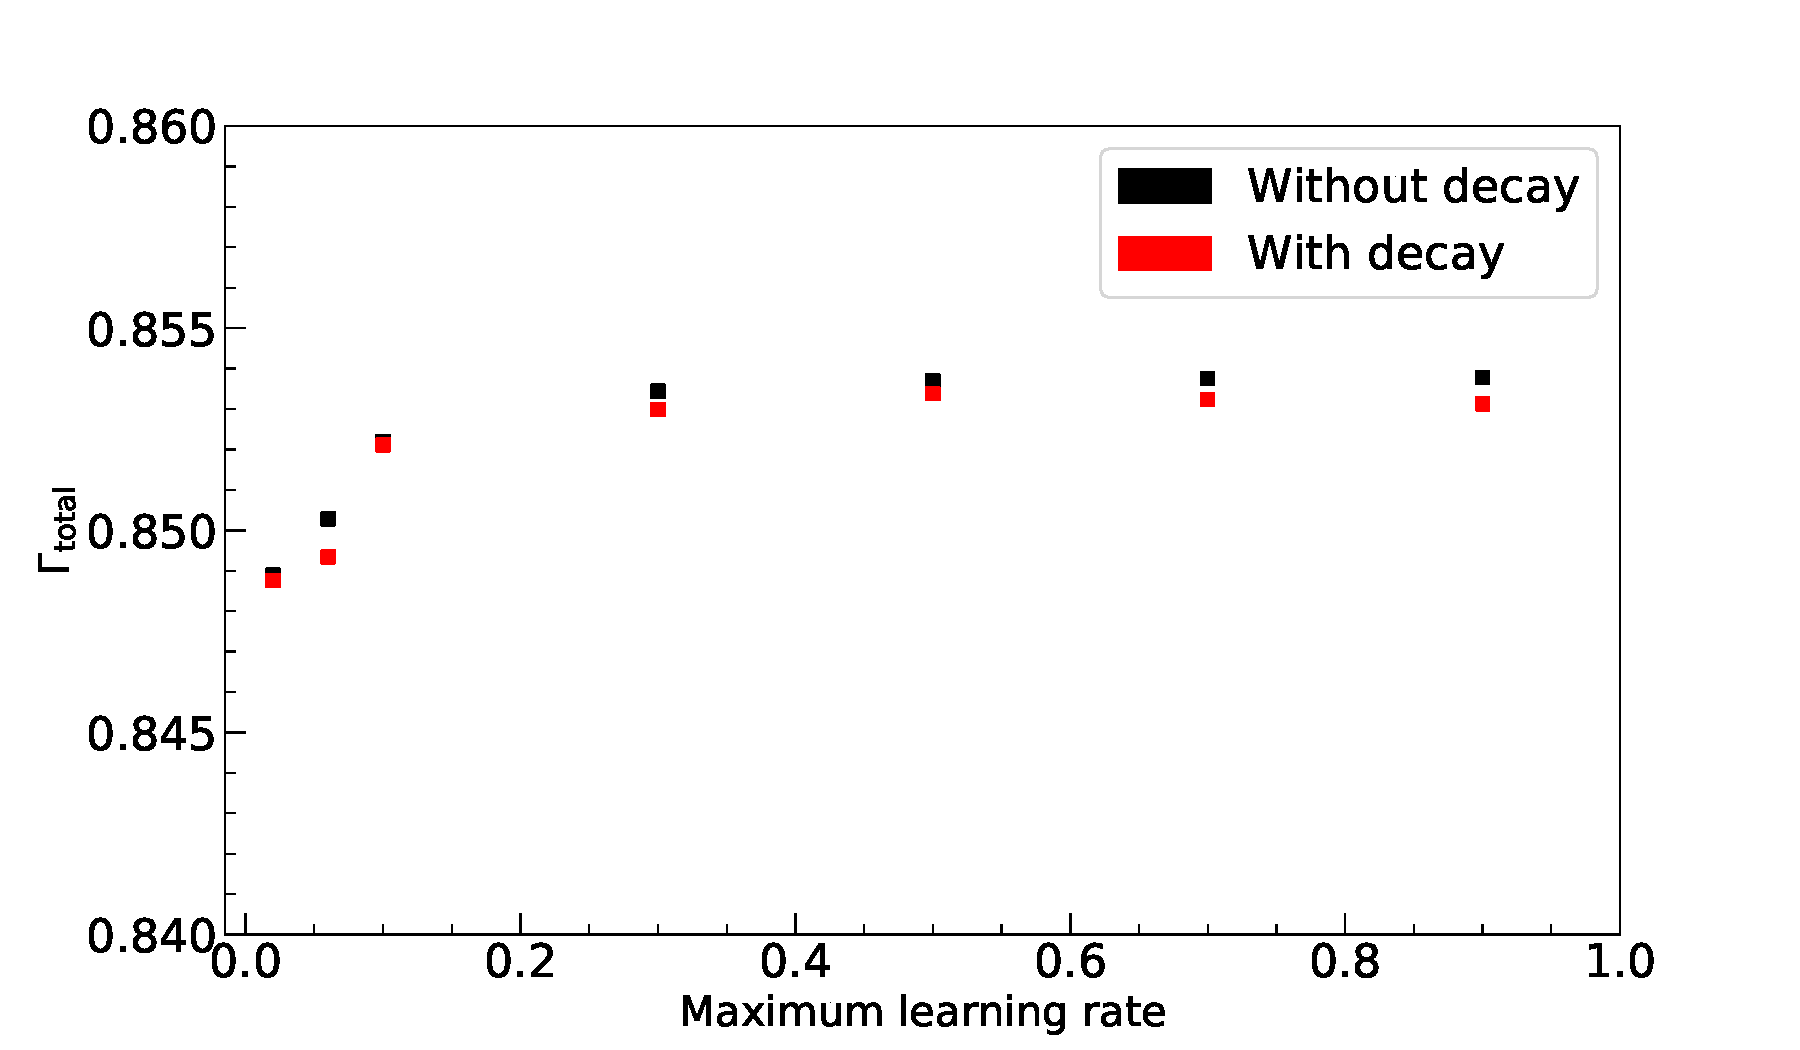
\includegraphics[width=0.95\linewidth]{figs/FNN/MaxAuc_Fixed}
\caption{The observed AUCs for different maximum learning rate using cyclic decay with and without additional decay.}
\label{fig:CylicLr}
\end{figure}

\begin{figure}[H]
\centering
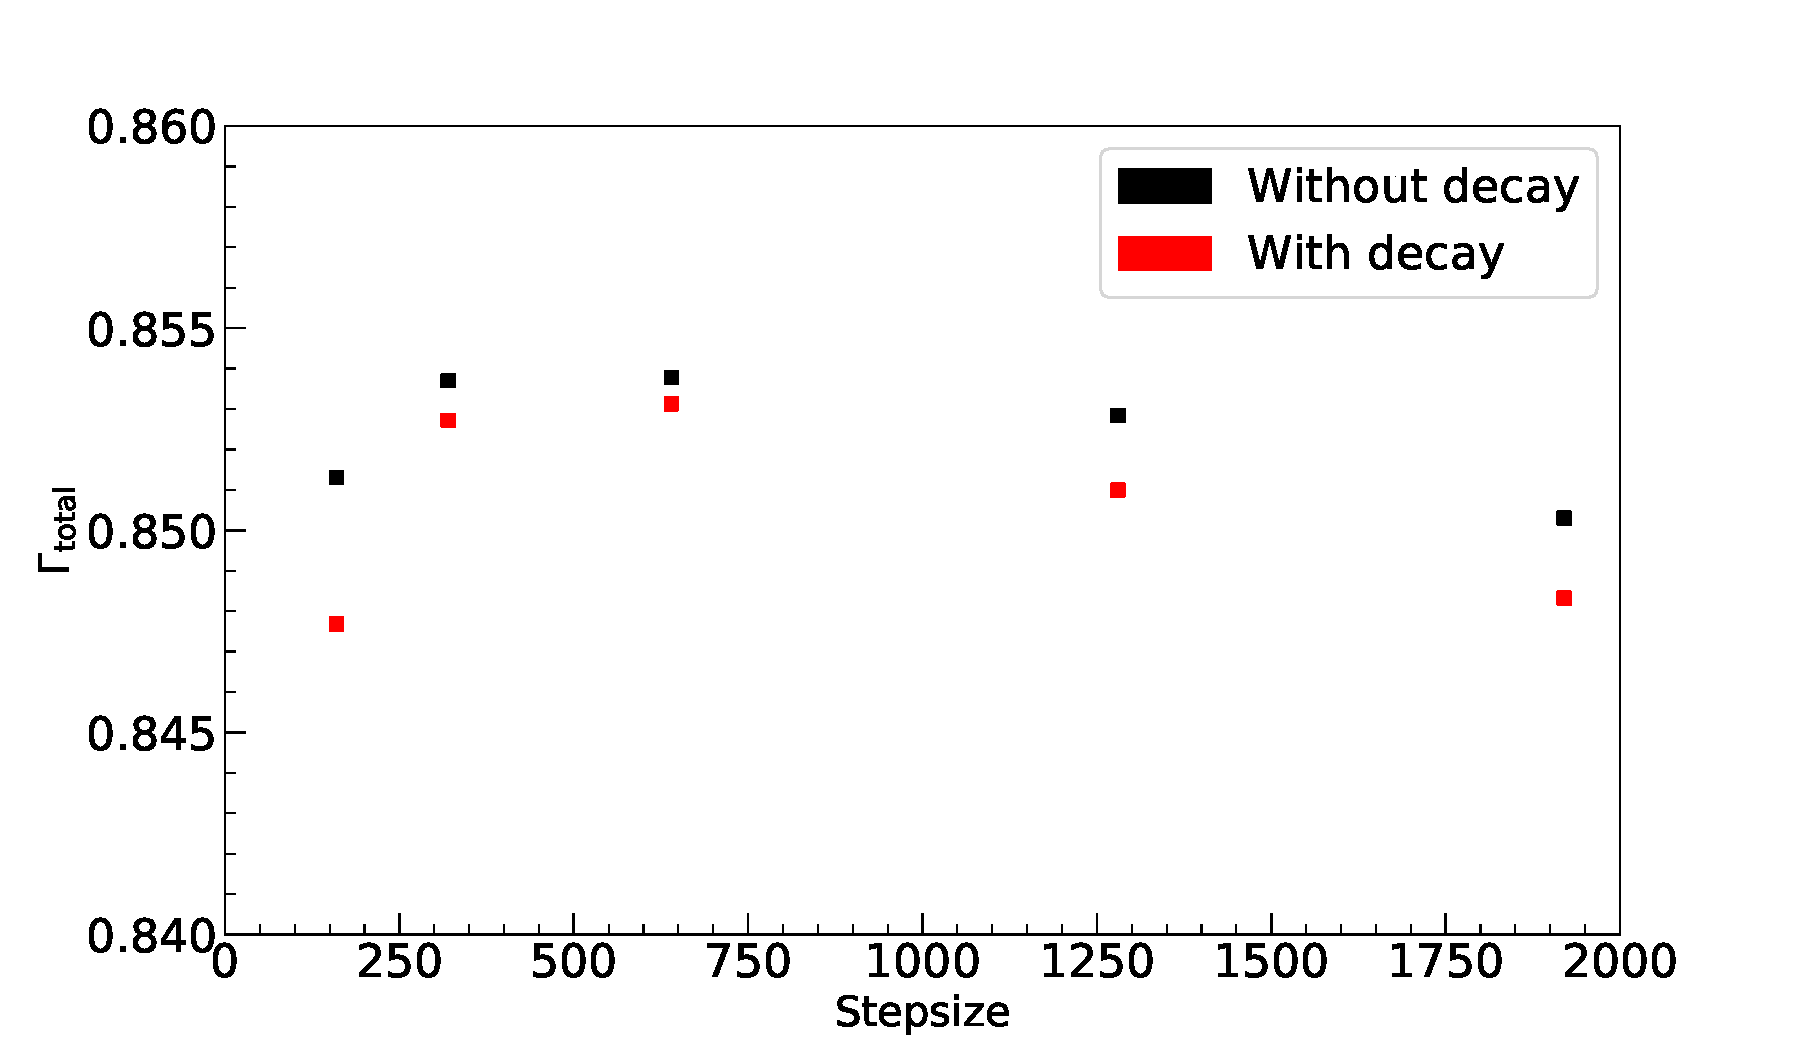
\includegraphics[width=0.95\linewidth]{figs/FNN/StepAuc_Fixed}
\caption{The dependence of the AUC on the stepsize chosen for the cyclic learning rate decay.}
\label{fig:CylicStepSize}
\end{figure}

Figure \ref{fig:CylicStepSize} shows obtained AUCs for the diverse stepsizes and different types of learning schedules. Stepsizes in the recommended region (between 160-640) result in the best AUCs while stepsizes below or above tend to decrease performance. The difference in performance between Neural Networks trained with the two distinctive learning rate schedules is small for stepsizes in the recommended region. Outside of the region, training without additional decay of the maximum learning rate works better. \\
The Neural Network with the best performance uses a constant maximum learning rate of 0.9, a minimum learning rate of 0.03, and a stepsize of 640. The obtained $\Gamma_{\text{total}}$ is 0.854 with an overtraining of 1.7\%.


\paragraph {Regularization} \mbox{} \\

The study of regularization aims to increase the AUC obtained on the testing dataset by decreasing the overtraining. Obtained models with under 2\% overtraining are already below the point of exceptions (5\%), and thus it is unlikely to obtain a higher AUC. \\
The two methods applied are the Dropout, govern by the probability $p$ for a neuron to be ignored during training and the Ridge regression, govern by $\alpha$ the scaling parameter of the additional Loss function term. The investigated values for $\alpha$ range from 0.001 (small regularization) to 0.1 (strong regularization) while the probability of Dropout is either 20\%, 40\%, or 60\%. The Dropout is only applied to the neurons in the hidden layer, giving the Neural Network the possibility of recovering performance during the training. To investigate the correlation between the learning rate and the different regularization methods, 5 different fixed learning rates between 0.0005 and 0.01 are investigated. The selected optimization algorithm is Adam since this optimization algorithm was used for the best-performing Neural Network in the fixed learning rate study. \\

\begin{figure}[H]
\centering
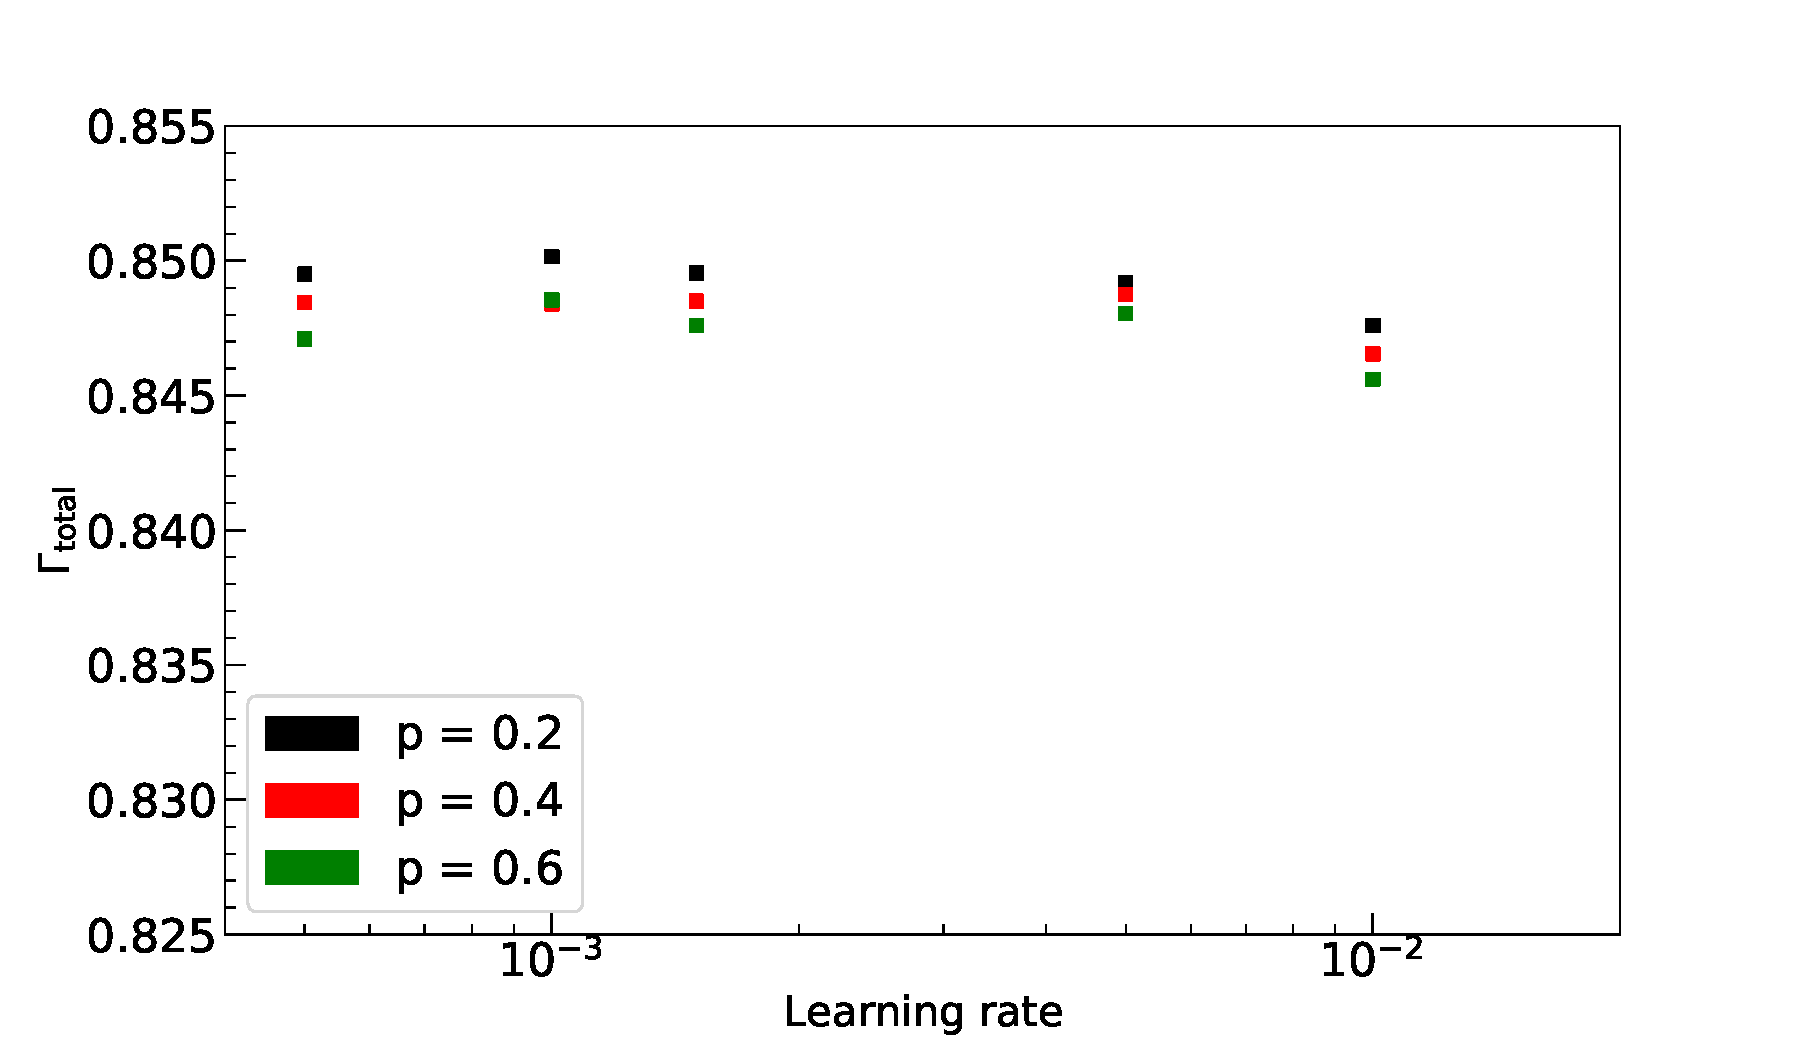
\includegraphics[width=\linewidth]{figs/FNN/Drop_Fixed}
\caption{Obtained AUCs for different learning rates and distinct choices of $p$, the Dropout probability.}
\label{fig:ReguDrop}
\end{figure}

Figure \ref{fig:ReguDrop} shows the obtained AUCs for the different learning rates and Dropout values, where $\alpha$ was fixed to 0.001. The peak performance has decreased by 0.003 compared to the results obtained without any regularization (cf. Figure \ref{fig:LrAuc}). Neural Networks with a lower probability of Dropout outperform those with a higher probability of Dropout as is to be expected for a regularization method. This behavior is also apparent in Figure \ref{fig:Regu}, where the learning rate is fixed to 0.001. The performances decrease continuously from the top left corner, where only little regularization is applied to the bottom right corner, where a strong regularization is applied. The overtraining of the trained Neural Networks, shown in Figure \ref{fig:ReguOv}, decreases with the amount of regularization applied as intended. \\
In the investigated parameter range, a large Ridge regression term is a stronger restriction than dropping out neurons in the first hidden layer with a high probability.

\begin{figure}[H]
\begin{subfigure}{.5\textwidth}
  \centering
  \includegraphics[width=.99\linewidth]{figs/FNN/Heat_l2DropAuc}
  \caption{}
  \label{fig:ReguLr}
\end{subfigure}%
\begin{subfigure}{.5\textwidth}
  \centering
  \includegraphics[width=.99\linewidth]{figs/FNN/Heat_l2DropOv}
  \caption{}
  \label{fig:ReguOv}
\end{subfigure}
\caption{The dependence of the AUC (a) and the overtraining (b) for different Dropout probabilities and l2 (Ridge) regularization.}
\label{fig:Regu}
\end{figure}


\paragraph{Achieved Separation} \mbox{} \\

\begin{figure}[H]
\begin{subfigure}{.5\textwidth}
  \centering
  \includegraphics[width=.99\linewidth]{figs/FNN/ScoreFNN19Even}
  \caption{}
  \label{fig:ScoreEven}
\end{subfigure}%
\begin{subfigure}{.5\textwidth}
  \centering
  \includegraphics[width=.99\linewidth]{figs/FNN/ScoreFNN19Odd}
  \caption{}
  \label{fig:ScoreOdd}
\end{subfigure}
\caption{Observed Neural Network scores for the Neural Network trained with the background dataset containing even event numbers (a) and on the background dataset constraining odd event numbers (b).}
\label{fig:Scores}
\end{figure}

The Neural Network obtained in the sub-section about cyclic learning rate decay is the best-performing model obtained for the $t\bar{t}t\bar{t}$ application. The score for the training on the dataset containing the background events with even event numbers is shown in Figure \ref{fig:ScoreEven}, whereas the score for the training on the dataset containing the background events with odd event numbers is shown in Figure \ref{fig:ScoreOdd}. Both classifications assign most signal events to scores above 0.7, and background events scores below 0.5. This indicates that the Neural Network is better at identifying signal events than at identifying background events, which is expected since the background dataset contains many different processes. The distance in each bin between the dots and the solid lines is related to the overtraining of the model. Since the Neural Network used has a tiny overtraining, most dots and lines are very close. \\

\begin{figure}[H]
\begin{subfigure}{1\textwidth}
  \centering
  \includegraphics[width=.93\linewidth]{figs/FNN/HT_all_Even}
  \caption{Dataset with even numbered background events}
  \label{fig:HTEven}
\end{subfigure} \\
\begin{subfigure}{1\textwidth}
  \centering
  \includegraphics[width=.93\linewidth]{figs/FNN/HT_all_Odd}
  \caption{Dataset with odd numbered background events}
  \label{fig:HTOdd}
\end{subfigure}
\caption{$H_{\text{T}}$ distributions after applying a cut (optimized on the signal efficiency) to the FNN scores obtained for the training on the background dataset containing even event numbers (a) and the background dataset constraining odd event numbers (b). The last bin additionally contains all events with $H_{\text{T}} > 2200$.}
\label{fig:HTFNN}
\end{figure}

To investigate which backgrounds are particularly hard to separate from the $t\bar{t}t\bar{t}$, a cut on the scores is optimized based on the signal efficiency. For both trainings the optimal cut is determined to be 0.7 which increases the signal efficiency in the signal region from 1.8 to 3.0. The $H_{\text{T}}$ distributions for the two cases are shown in Figure \ref{fig:HTFNN}. The dominant backgrounds after applying the cut are still $t\bar{t}W$, $t\bar{t}Z$ and $t\bar{t}H$. The model trained on the backgrounds with even event numbers is better in rejecting $t\bar{t}CO$ while the model trained on the backgrounds with odd event numbers is better in rejecting $t\bar{t}$others. However, the difference is minor and therefore most likely a coincidence. The rejection of all other backgrounds is approximately equally good for both setups when normalized to the signal yield in the investigated region. The signal yield is reduced by a factor of 2 while most other backgrounds are reduced by a factor of $\sim 25$. The background  yield of the dataset ``others'' mainly containing $t\bar{t}t$ is the background that is hardest to distinguish from $t\bar{t}t\bar{t}$ and is only reduced by a factor of 3. A similar result was obtained by the BDT used in the official ATLAS $t\bar{t}t\bar{t}$ analysis at $\sqrt{s} = \SI{13}{TeV}$ which used the same datasets. In fact, for the high BDT region a significant $t\bar{t}t$ contamination was observed. This can be especially problematic because the $t\bar{t}t$ cross section, is only known at leading order $\sigma_{t\bar{t}t} = \SI{1.9}{fb}$ (at $\sqrt{s} = \SI{14}{TeV}$) \cite{3t}. If the  $\sigma_{t\bar{t}t}$ at NLO is higher than the LO cross section $t\bar{t}t$ could become the dominant background for $t\bar{t}t\bar{t}$. \\

\paragraph{Validation and Error Estimation} \mbox{} \\

\begin{figure}[H]
\centering
\includegraphics[width=\linewidth]{figs/FNN/BootStrap}
\caption{AUCs observed by using the bootstrap method on the validation set. The seed quoted (times 365) is the random seed used to generate the different resampled versions of the validation set. The red line indicates the mean of all observed AUCs.}
\label{fig:BootStrapFNN}
\end{figure}

As mentioned preciously in Section \ref{sec:splitting} the generalization of the optimized Neural Network has to be validated on the restrained validation dataset. The error of observed AUC can than be obtained by boostrapping. The selected number of resampled datasets is 50. \\
The bootstrapping results for the selected Neural Network performed on the validation set is shown in Figure \ref{fig:BootStrapFNN}. The seed quoted on the x-axis is the random seed (times 365) used for resampling the validation set. The average of all 50 AUCs obtained is indicated by the red line.
The obtained average $\Gamma_{\text{total}}$  is $0.852 \pm 0.005$, where the error is the standard deviation of the obtained distribution. The error is larger than the performance gained by fine-tuning the learning rate within one order of magnitude. The AUC achieved on the testing set ($0.854$) is within the error observed by bootstrapping. This means during the hyperparmeter optimization no addition bias was introduced.


\newpage

\section{Multi Classification using Feedforward Neural Networks}
\label{sec:Multi}

The Feedforward Neural Networks trained in the last section had one neuron in the output layer and classified signal events against background events. The Neural Networks considered in this section all have several neurons in the output layer in order to individually treat different background processes. The outputs of the Neural Network are $M$ probabilities, where $M$ is the number of classes considered. Each probability is the likelihood of the given event to belong to a class $c$. Two different multi classifications will be investigate in the following one with 14 classes and on with 3 classes. \\
The AUCs quoted in the following sub-section are calculated in the same way that AUCs were calculated for the binary classification approach (single against all combined backgrounds). The number of parameters is increased to approximately 300000 to account for the increased complexity of the problems considered.\\
For convenience, $V$ is redefined excessively for this section to be either a $W$, a $Z$, or a Higgs boson.

\paragraph{Fourteen Classes} \mbox{} \\

\begin{figure}[H]
\begin{subfigure}{.55\textwidth}
  \centering
  \includegraphics[width=.99\linewidth]{figs/MultiClass/Cm_unweighted}
  \caption{}
  \label{fig:CMunW}
\end{subfigure}%
\begin{subfigure}{.45\textwidth}
  \centering
  \includegraphics[width=.99\linewidth]{figs/MultiClass/Score_tttt_ttWothers}
  \caption{}
  \label{fig:Score14}
\end{subfigure}
\caption{The confusion matrix (a) and the Neural Network score (b) for the multi classification with 14 classes.}
\label{fig:14Class}
\end{figure}

The first multi classifier approach treats every background process as an individual class. Presenting the Neural Network with the opportunity to optimize the selection for each background. The best obtained $\Gamma_{\text{total}}$ is 0.852 and it did not increase the performance compared to the binary classification used previously. \\
Figure \ref{fig:Score14} shows the score for the most important backgrounds. The similarity between the $t\bar{t}t\bar{t}$ (red) and the $t\bar{t}t$ (green) observed in Section \ref{sec:FNN_results} is apparent since the highest fraction of events for both processes end up in highest bins. The dominant backgrounds $t\bar{t}V$ (blue) are most commonly assigned a score below 0.5 but also have considerable contributions up to scores of 0.8. All other backgrounds (black) have a similar distribution to $t\bar{t}V$. \\
In Figure \ref{fig:CMunW} the confusion matrix of the obtained classification is shown. The y-axis gives the information about the true event class. The predicated labels on the x-axis are determined by assigning an event to the class for which it has the highest probability. The numbers given in the different cells correspond to fractions of total events in the same row or column. A perfect classification would only have entries of 1 on the diagonal. The trained classifier has almost exclusively entries for three classes, which correspond to the processes with the highest yields. The $t\bar{t}t\bar{t}$ yield was renormalized to the combined total background yield as discussed in Section \ref{sec:transformation}. Therefore, it is beneficial for the Neural Network to focus on the correct identification of  $t\bar{t}t\bar{t}$ events rather than rejecting background events.

\newpage

\paragraph{Class Weights} \mbox{} \\

\begin{figure}[H]
\centering
\includegraphics[width=\linewidth]{figs/MultiClass/Cm_classweights}
\caption{The confusion matrix for the multi classification with 14 classes where an additional class weight was applied during the training of the Classifier.}
\label{fig:CMWed}
\end{figure}

A way to force the neural network to pay more ``attention'' to minor backgrounds is to scale all processes to the same yield using class weights. This reweighting will decrease the AUC of the obtained classification. However insights about which backgrounds are most difficult to distinguish for $t\bar{t}t\bar{t}$ can be gained. Thus, providing a possibility to validate the observations about $t\bar{t}t$ (others). The class weights $w_{c}$ are calculated according to
\begin{equation}
w_{c} = \frac{N_{\text{total}} }{M \cdot N_{c}}
\end{equation}
where $N_{\text{total}}$ is sum of all yields and $N_{c}$ is the yield of class $c$. \\
The confusion matrix obtained by applying class weights is shown in Figure \ref{fig:CMWed}. As intended, most classes have their largest fraction of events on the diagonal. The separation between different classes is limited by the choice of the input variables that were selected to discriminate signal from all backgrounds and not to discriminate between different backgrounds individually. In agreement with the previous studies, the dataset ``others'' is the background with the highest fraction of events predicted to be signal events (0.4). The other signal like backgrounds for this classification are $t\bar{t}H$ and $t\bar{t}WW$.

\newpage

\paragraph{Three Classes} \mbox{} \\

In this approach, only three different classes are considered, namely a signal class, a class containing the most dominant backgrounds $t\bar{t}V$, and a class for all other backgrounds called ``rest''. No additional class reweighting is applied. This study aims to improve the AUC compared to the result obtained in the binary approach. The additional class of $t\bar{t}V$ is meant to help further reduce the dominant background.

\begin{figure}[H]
\begin{subfigure}{.55\textwidth}
  \centering
  \includegraphics[width=.99\linewidth]{figs/MultiClass/CmOther}
  \caption{}
  \label{fig:CM3}
\end{subfigure}%
\begin{subfigure}{.45\textwidth}
  \centering
  \includegraphics[width=.99\linewidth]{figs/MultiClass/ScoreFNN14Even_0}
  \caption{}
  \label{fig:Score3}
\end{subfigure}
\caption{The confusion matrix (a) and the Neural Network score (b) for the multi classification with 3 classes.}
\label{fig:3Class}
\end{figure}

The results of this approach is shown in Figure \ref{fig:3Class}. The events belonging to the ``rest'' class are identified as a signal or $t\bar{t}V$ event. This is because this class has a low combined yield of $\sim 86$ whereas $t\bar{t}V$ has a yield of 151 and $t\bar{t}t\bar{t}$ a yield of 237, during training. The identification of $t\bar{t}V$ has significantly improved compared to the previous multi classifier approaches. On the other hand, the identification of $t\bar{t}t\bar{t}$ has decreased from 0.94 (cf. Figure \ref{fig:14Class}) to 0.87. \\
The observed AUC for the classification with three classes is 0.854. This result seems to be contradict to the result of the binary classification approach with a AUC 0.853 where in the high score region (cf. \ref{fig:HTFNN}) better rejections of $t\bar{t}V$ and all the remainder backgrounds than 0.37 and 0.6 were found. However, the confusion matrix in Figure \ref{fig:CM3} assigns the event to the most likely category. Reviewing the background events ending up in the $t\bar{t}t\bar{t}$ category showed that most of them had scores below 0.8 but higher scores for $t\bar{t}t\bar{t}$ than for the other two categories.

\newpage


\section{Signal Classification using Recurrent Neural Networks}
\label{sec:RNN_results}

Compared to Feedforward Neural Networks, Recurrent Neural Networks are more complicated to train and more computationally expensive. A single neuron of the used LSTM neuron structure has 5 activation functions, each of which has specific functionalities that control the different cell states. Therefore, they different choices for this activation functions will not be considered. \\
The strategy chosen to study RNNs is restricted to the most impactful parameters, namely the number of parameters, the number of hidden layers, and the learning rate. The optimization algorithm selected is SGD and it is used in combination with polynomial learning rate decay to ensure that the training converge if a minimum is found in the parameter space. The maximum number of Epochs is restricted to 80, while the AUC is computed at every Epoch. The mean and the standard deviation needed to transform the input features are obtained based on all objects in the considered feature. To be more concrete, to transform the leading electron's pseudorapidity into a normal distribution, the $\eta$ of all electrons is considered during the calculation of mean and standard deviation. Only the 7 objects with the highest $p_{\text{T}}$ for each particle type and event are considered to avoid using variables with significant mismodeling. Since several of the $ 7 \cdot 13 = 84$ input features contain many zeros (due to zero padding), Lasso regression must be applied. The scaling constant $\alpha_1$ is fixed to 0.002.


\paragraph{Architecture} \mbox{} \\

\begin{figure}[H]
\centering
\includegraphics[width=\linewidth]{figs/RNN/AucPara_RNN}
\caption{The average overtraining for different RNNs configurations. The training is stopped after 20, 40, 60 and after 80 Epochs. The average includes the overtrainings of the 4 best-performing Neural Networks of different depth.}
\label{fig:ParaRNN}
\end{figure}


As for the FNNs, the number of parameters and the number of layers is investigated first. Based on the knowledge gained in the first architecture study (Section \ref{sec:FNN_results}), the range for the number of parameters considered is between 2000 and 30000. The number of hidden layers tested is restricted to a maximum of 4 hidden layers. \\
Figure \ref{fig:ParaRNN} shows the AUCs of Neural Networks with varying number of trainable parameters obtained at 20 (black), 40 (red), 60 (blue), and 80 (green) Epochs. Every quoted $\Gamma_{\text{total}}$ is average over the 4 different hidden layer configurations considered. The performance for 40, 60, and 80 Epochs is similar for the most studied sizes, while the training at 20 Epochs has not converged yet. The Neural Networks with 30000 parameters evaluated at Epoch 80 show a decrease in performance, which hints to the fact that these models started to overtrain. \\
Almost all models have an overtraining below 3\%, implying that the applied regularization is sufficient. The overtraining is independent of the number of parameters and hidden layers in the Neural Networks, which indicates that all trainings converged. \\
The Neural Networks with 1 or 2 hidden layers outperformed Neural Networks with 3 or 4 hidden layers in all cases considered. The peak performance of $\Gamma_{\text{total}} = 0.838$ is reached by a Neural Network with 15000 parameters and two hidden layers.

\paragraph{Learning Rate and Batch size} \mbox{} \\

\begin{figure}[H]
\centering
\includegraphics[width=\linewidth]{figs/RNN/LrAuc_Fixed}
\caption{The obtained average AUC of RNNs with different learning rates. The average includes the AUCs of the 2 best-performing Neural Networks with different batchsizes.}
\label{fig:LrRNN}
\end{figure}

The Neural Network with the best performance in the previous study is selected to investigate the AUCs dependence on the learning rate and the batch size. The considered batch size reaches from $10^{11}$ to $10^{14}$, which was observed to be a high-performance region for FNNs. Following the same logic, learning rates between 0.05 and 0.8 with decay polynomials of power 1 to 3 are selected. \\
Figure \ref{fig:LrRNN} shows the average AUCs obtained using the different learning rates and decay polynomials. The average includes the results for the two best performing considered batch sizes (2048 and 4096). Similar to the observed results for FNNs, the performance of RNNs is stable within one order of magnitude around the learning rate that performs the best. Outside of the stable region, it decreases the performance of RNNs rapidly. Similarly, the power of the chosen polynomial has a minor influence on the performance inside the stable region, whereas outside of the region, it can have a significant influence.  One reason for this could be the more complex and thus more fragile training procedures for RNNs compared to FNNs. On the other hand, the fact that the learning rate decay of order 1 worked the best implies that the Neural Networks might not have converged. The Epoch at which the highest AUC is reached is close to the maximum 80 Epochs but more than 5 Epoch away. Therefore, a combination of both effects is the most likely explanation for the rapid drop. \\

\begin{figure}[H]
\centering
\includegraphics[width=\linewidth]{figs/RNN/BatchOv_Fixed}
\caption{The AUC as a function of the batch size and the learning rate.}
\label{fig:BatchRNN}
\end{figure}

The dependence of the AUC on the batch size is shown in Figure \ref{fig:BatchRNN}. A similar dependence as for the FNNs can be observed. For learning rates close to the optimal value obtained, the batch size has a minor influence on the performance of the Neural Networks. For smaller learning rates, the dependence is larger. The decrease in performance when choosing a large batch size, when combined with a small learning rate, is larger than the observed decrease for FNNs. This validates the assumption that the more complex training of RNNs is sensitive to the choice of hyperparameters. \\
The best performing RNN has a significantly smaller AUC (0.842) than the best performance observed using FNNs (0.854). Therefore, the initial idea to present the Neural Network with the possibility of using the full information available did not improve $\Gamma_{\text{total}}$. The RNN failed in combining the input features in a way that discriminates the signal from the background more than the features used for FNNs, which are constructed using physical knowledge. \\
The overtraining of all considered Neural Networks is below 3\%. Figures showing the dependence of overtraining on the batch size and the learning rate can be found in Appendix \ref{ap:addRNN}.

\newpage

\paragraph{Achieved Separation} \mbox{} \\

\begin{figure}[H]
\centering
\includegraphics[width=\linewidth]{figs/RNN/HT_all_Even}
\caption{The $H_{\text{T}}$ distribution after applying a cut (optimized on the signal efficiency) to the RNN score obtained for the training on the background dataset containing even event numbers. The last bin additionally contains all events with $H_{\text{T}} > 2200$.}
\label{fig:RNNHT}
\end{figure}


Proceeding in the same way as for the FNNs, a cut based on the signal efficiency is optimized on the RNN score. Events passing that cut contribute to the $H_{\text{T}}$ distribution shown in Figure \ref{fig:RNNHT}. The selected RNN is the best-performing Neural Network from the learning rate and batch size study in the previous sub-section. It was trained on the background dataset, which contains events with odd event numbers. The score of the RNN can be found in the Appendix \ref{ap:addRNN} together with both the score and the $H_{\text{T}}$ distribution of the corresponding RNN trained on background events with odd event numbers. \\
The optimized cut is determined to be 0.85. The signal efficiency in the signal region improves from 1.8 to 2.7. As expected, is this signal efficiency lower than the one observed for the best FNN (2.9). The comparison between the background yields after applying the respective cuts to the FNN and RNN scores is shown in table \ref{tab:Rejcomb} where $\kappa$ and $\zeta$ are functions of the signal efficiencies $s$ and are calculated according to
\begin{equation}
\kappa = s \cdot Y'_{\text{sig}} 
\label{eq:kappa}
\end{equation}
\begin{equation}
\zeta = \frac{\kappa_{\text{FNN}} - \kappa_{\text{RNN}}}{Y_{\text{sig}}}
\label{eq:zeta}
\end{equation}
where $Y'_{\text{sig}}$ is the signal yield after applying the cut and $Y_{\text{sig}}$ before. As can be seen, the reduction measure $\kappa$ of all backgrounds is higher for FNN than for RNNs. The background hardest to reduces is $t\bar{t}t$. The dominate background $t\bar{t}W$, $t\bar{t}Z$ and $t\bar{t}H$ are reduced the most. $\zeta$ was designed with the intend to investigate from which backgrounds the performance decrease of the RNN, compared to the FNN, originates from. The backgrounds $VV$ and $t(\bar{t})X$ have the highest $\zeta$ values which indicates that these background especially benefit from the engineered features in the FNN. 

\begin{table}[H]
\begin{tabular}{|r|r|r|r|r|r|r|r|r|r|r|r|}
\toprule
measure & $t\bar{t}W$ & $t\bar{t}Z$ & $t\bar{t}H$ & $t\bar{t}$QmisID & $t\bar{t}$CO & $t\bar{t}$HF & $t\bar{t}$light & $t\bar{t}$other & $t(\bar{t})X$ & $VV$ & others \\
\midrule
\midrule
$\kappa_{\text{FNN}}$ & 33.8 & 33.6 & 33.7 & 53.1 & 45.5 & 68.9 & 111.3 & 74.7 & 100.8 & 197.7 & 59.4 \\
$\kappa_{\text{FNN}}$ & 29.4 & 29.2 & 29.3 & 46.2 & 39.6 & 60.0 & 96.9 & 65.0 & 87.7 & 172.0 & 51.7 \\
$\zeta$ & 0.07 & 0.09 & 0.11 & 0.51 & 0.27 & 0.56 & 2.15 & 1.54 & 2.55 & 5.84 & 2.52 \\
\bottomrule
\end{tabular}
\caption{The reduction measure $\kappa$ (defined in Equation \ref{eq:kappa}) for the high FNN and RNN region and there scaled difference $\zeta$ (defined in Equation \ref{eq:zeta}).}
\label{tab:Rejcomb}
\end{table}

\paragraph{Validation and Error Estimation} \mbox{} \\

\begin{figure}[H]
\centering
\includegraphics[width=\linewidth]{figs/RNN/BootStrap_RNN}
\caption{AUCs observed by using the bootstrap method on the validation set. The seed quoted (times 365) is the random seed used to generate the different resampled versions of the validation set. The red line indicates the mean of all observed AUCs.}
\label{fig:RNNBootStrap}
\end{figure}

The obtained AUC on the testing dataset (0.842) needs to be validated to 
ensure that no additional bias during the hyperparameter tuning was introduced. As for the FNN, the validation realized by obtaining the AUC on the resampled versions of the validation sample. Figure \ref{fig:RNNBootStrap} shows the observed AUCs and there mean value (red line) $\Gamma = 0.838$. The standard deviation represents the error of the obtained result and was determinate to be 0.006. Therefore, is the observed performance on the testing set within the exacted error.


\newpage

\section{Performance Evaluation of CPUs and GPUs}
\label{sec:CPUGPU}

All Neural Networks used in the previous studies were trained on Central Processing Units (CPUs). However, in deep learning applications, it is prevalent to use Graphics Processing Units (GPUs). \\
Most operations performed during a Neural Network training are simple matrix multiplication of weight matrices and feature matrices. CPUs are designed to perform few but complicated tasks and struggle with multiple threads at the same time. On the other hand, GPUs are designed to perform simple but many tasks at the same time, making them the optimal choice for deep learning applications. \\
The following study investigates the training time of Feedforward Neural Networks and Recurrent Neural Networks using CPUs and GPUs.
The same datasets that were used in the previous Neural Network studies are utilized in here. The devices used for the training are Intel Xeon e5-2620 v3 CPUs and Geforce gtx 1080 GPUs. \\
Neural Networks with sizes between 2000 and 70000 parameters are considered. The optimization algorithm used is SGD, with batch sizes between $2^{10}$ and $2^{16}$. All other parameters are fixed to the best-performing Neural Networks of each type. The AUC evaluation at each Epoch is turned off since the needed calculations can take several seconds. The reported train time per Epoch is the average over 120 Epochs. \\

\begin{figure}[H]
\centering
\includegraphics[width=\linewidth]{figs/CPUGPU/NumParaTraintime_Fixed}
\caption{Training times per Epoch for FNNs and RNNs of different sizes trained on CPUs and GPUs.}
\label{fig:CPUGPUPara}
\end{figure}

Figure \ref{fig:CPUGPUPara} shows training time for the Neural Networks of different sizes where the batch size was fixed to 8192. The RNNs take significantly longer to train than the FNNs due to their more complicated neuron structure and training algorithm. GPUs outperform CPUs for all considered Neural Networks. The gain in performance is especially high for Neural Networks with many tunable parameters. For the largest RNNs training time decreases per Epoch by a factor of 4 when using GPUs compared to CPUs. \\
The results for the different batch sizes are shown in Figure \ref{fig:CPUGPUBatch}, where a Neural Network with 50000 parameters was used. Again GPUs outperform CPUs over the full parameter space selected. The decrease in training time is small for small batch size and increases with larger batch sizes. The reason for this is that only the calculations within one iteration are performed simultaneously. Since the number of performed calculations scale with the batch size, also the performance gain does. The saturation of performance gain for Neural Networks with batch size larger than $\sim16000$ most likely has two sources. The first one being that for this batch sizes the matrices get so large that the GPUs reach their limit in terms of maximum number of calculations that can be performed at the same time. The second possible explanation is the observed standard deviation of the training times per Epoch was significantly higher for the batches of $2^{15}$ and $2^{16}$. This indicates that the cluster node started to lag, potentially influencing the obtained result. \\
In conclusion it can be stated that even for the small datasets and Neural Networks considered, the usage of GPUs is highly advisable.

\begin{figure}[H]
\centering
\includegraphics[width=\linewidth]{figs/CPUGPU/BatchTraintime_Fixed}
\caption{Training times per Epoch for FNNs and RNNs trained with different batch sizes and on CPUs and GPUs.}
\label{fig:CPUGPUBatch}
\end{figure}

\newpage

\section{Reconstruction of Two Hadronic Top Quarks}
\label{sec:TwoHadTop}

The $t\bar{t}t$ contamination in the high score regions of the FNN, the RNN, and the BDT used in the official $t\bar{t}t\bar{t}$ analysis motivate the search for a feature that discriminates the two processes well. Since both processes are very similar in their kinematics, the chosen approach aims at the final state particle composition. In the same-sign two lepton channel, two of the four $W$ bosons that originate from four top quark decays, decay
hadronically. On the other hand, a $t\bar{t}t$ event produced without any associated particles has one hadronically decaying W boson in the final state. As discussed in Section \ref{sec:Theory3top} such a production is not possible at leading order. In practice make the particles produced in association with the $t\bar{t}t$ the separation of $t\bar{t}t\bar{t}$ and $t\bar{t}t$ more complicated. Incorrect reconstruction of jets or leptons and charge misidentification can further disturb a possible reconstruction. \\
The datasets used for the reconstruction were introduced in Chapter \ref{sec:Samples}. The signal region is redefined to match the conditions of the two hadronic top quark reconstruction. Events with 3 or more leptons are rejected; only events with two leptons with charges have the same sign are considered. The number of required jets is raised from at least 6 jets to at least 8 jets. All other signal region conditions stay the same.

\paragraph{Reconstruction principle} \mbox{} \\

The reconstruction technique presented in the following tries to identify $t\bar{t}t$ events by final states that have one hadronic top quark and $t\bar{t}t\bar{t}$ events by final states that have two hadronic top quark. Priority is given to the reconstruction of two hadronic top quarks, which are reconstructed from 6 jet combinations, 3 jets for each top quark. At least one of the two top quark candidates has to contain a b-jet. The assignment of the three jets to a W boson and a b-jet depends on the number of b-tagged jets contained within the top quark. If only one of the jets is b-tagged, this jet is assigned to the b-jet, and the two other jets are said to be the decaying produces of the W boson. If two jets are b-tagged, the two jet combination with the lowest discriminator is selected, but at least one b-tagged jet has to be assigned to the b-jet. If non or all jets are b-tagged, the combination with the lowest discriminator is selected. \\  
The discriminator chosen for the reconstruction is based on $\chi^2$ and contains one term for each of the four reconstructed objects (2 top quarks and 2 W bosons). 
\begin{equation}
\label{eq:Chi2had}
\chi^2_{\text{2had}} = \chi^2_{t_1} + \chi^2_{t_2} + \chi^2_{W_1} + \chi^2_{W_2}
\end{equation}
The individual $\chi^2$ terms are defined as
\begin{equation}
\label{eq:Chi2}
\chi^2_X = \frac{(m_{3/2j} - m_X)^2}{\sigma_X^2}; \,\,\,\,\,\, X \in {t,W}
\end{equation}
where $m_{3/2j}$ is the mass of the 3 or 2 jet combination. The mass and the width of the top quark and the W boson are obtained from the dataset, which will be discussed in the next sub-section. \\
The reconstruction of two hadronic top quarks is defined to be successful if $\chi^2_{\text{2had}}$ does not exceed a critical value $\chi^2_{c1}$. The exact value of $\chi^2_{c1}$ is left as a tunable parameter of the reconstruction. If $\chi^2_{\text{2had}}$ is smaller than the $\chi^2_{c1}$, the reconstruction of one hadronic top quark is carried out. The reconstruction of one hadronic top quark proceeds in the same way as the two hadronic top quark reconstruction using the discriminator $\chi^2_{\text{1had}} = \chi^2_{t_1} + \chi^2_{W_1}$. If $\chi^2_{\text{1had}}$ surpasses a second critical value $\chi^2_{c2}$, the event is considered to have no hadronic top quark.

\newpage

\paragraph{Calibration} \mbox{} \\

\begin{figure}[H]
\begin{subfigure}{.5\textwidth}
  \centering
  \includegraphics[width=.99\linewidth]{figs/HadTop/TopMass}
  \caption{Top Quark}
  \label{fig:Calt}
\end{subfigure}%
\begin{subfigure}{.5\textwidth}
  \centering
  \includegraphics[width=.99\linewidth]{figs/HadTop/WMass}
  \caption{$W$ boson}
  \label{fig:CalW}
\end{subfigure}
\caption{Mass distributions of the truth matched and reconstructed top quarks (a) and W bosons (b).}
\label{fig:Cal}
\end{figure}

The calibration of the top quark and W boson mass and width is performed by matching the reconstruction candidate to the \textit{truth particles}. The kinematic and final state particles of the truth particles are known from the truth information in the used datasets. Only hadronically decaying truth top quarks or W bosons with final state particles that can be measured by the ATLAS detector are considered. The matching is performed based on the $\Delta R$ between the reconstruction candidates and the truth top quarks in the same event. The closest reconstruction candidate is assigned to the truth top quark. The matching of W bosons is performed in the same way and independently of the matching of top quarks. \\
Only matched pairs that have a $\delta R(\text{reco},\text{truth})$ smaller than the critical value are considered for the final mass fit. Figure \ref{fig:Cal} shows the result of the calibration with a critical value of $\delta R(\text{reco},\text{truth}) < 0.4$. The mass and the width of the particles is observed as the mean and standard deviation of the gaussian fit.  The obtained masses and width are $m_t = 172$, $m_W = 82$, $\sigma_t = 21$, and $\sigma = 9$. \\
To study the dependence of the observed masses and widths, different critical values between 0.1 and 0.8 were considered. The mean of the distribution is approximately independent of the critical value. The standard deviation varied between 22.6 and 16.9 for the top quark and between 7.7 and 9.6 for the W boson. The critical value of $\Delta R(\text{reco},\text{truth}) < 0.4$ was selected as the point at which both weight distributions showed an approximately symmetric peak. \\
In order to have a comparison to the results discussed in the next sub-section, a \textit{best-possible reconstruction} is defined. This reconstruction also uses truth information and, therefore, can not be used for measured data. All pre-requirement concerning the number of b-jets in the reconstructed particles are the same as for the $\chi^2$ based reconstruction. The best-possible reconstruction first selects all top quark candidates with a mass within $3\sigma$ around $m_t$ and contain a W candidate within $3\sigma$ around $m_W$. If there are more truth top quarks than reconstructed top quarks, the mass windows are broadened to $4\sigma$. If the number of truth top quarks still exceeds the number of reconstructed top quarks, all candidates are kept. After this pre-selection is finished, the matching based on $\delta R(\text{reco},\text{truth})$ as described previously is performed. The candidates closest to the truth top quarks in the same event are said to be the reconstructed top quarks.

\newpage

\paragraph{Reconstruction Results} \mbox{} \\


\begin{figure}[H]
\begin{subfigure}{.5\textwidth}
  \centering
  \includegraphics[width=.99\linewidth]{figs/HadTop/4topResult}
  \caption{$t\bar{t}t\bar{t}$ events}
  \label{fig:Reco4t}
\end{subfigure}%
\begin{subfigure}{.5\textwidth}
  \centering
  \includegraphics[width=.99\linewidth]{figs/HadTop/3topsResult}
  \caption{$t\bar{t}t$ events}
  \label{fig:Reco3t}
\end{subfigure}
\caption{Observed reconstruction where the critical values were tuned such that the fraction of events in all three channels fit the true $t\bar{t}t\bar{t}$ distribution.}
\label{fig:RecoResult}
\end{figure}

\vspace{-0.01cm}

Figure \ref{fig:RecoResult} shows the number of identified hadronic top quarks for the $t\bar{t}t\bar{t}$ and the $t\bar{t}t$ processes for the $\chi^2$ reconstruction (blue) and the true distribution (red). The critical values $\chi^2_{c1} = 5$ and $\chi^2_{c1} = 10$ are tuned such that the obtained results match the true $t\bar{t}t\bar{t}$ distribution. This results in a poor performance on the $t\bar{t}t$ dataset. In fact only 64\% of the events $t\bar{t}t\bar{t}$ and 43\% of the $t\bar{t}t$ events are categorized correctly to one or two hadronic top quark events. Most $t\bar{t}t$ one hadronic top quark events are reconstructed as two hadronic events and most non hadronic top quark events are reconstructed as one hadronic top quark events. The most likely explanation for this behavior is that the dominant production channel of $t\bar{t}t$ is associated production with a W boson. In fact, the original branching fraction of 0.72 is increased due to the signal region cuts to 0.99. In the case where the additional W boson decays hadronically, a hadronic top quark decay can be easily faked. The additional W boson is also the reason why at truth level not all $t\bar{t}t$ events in the signal region have one hadronic top quark. The signal region requirement of two same sign leptons can be achieved for a two hadronic $t\bar{t}t$ event when the additional W boson decays leptonically. \\
The poor performance (only 64\% of all events a categorized correctly) for the $t\bar{t}t\bar{t}$ is not apparent. The comparison of $\delta R(\text{reco},\text{truth})$ between the $\chi^2$ based reconstruction and the best-possible reconstruction, shown in Figure \ref{fig:dR}, shows that in most cases the incorrect jet combinations were selected. Furthermore, the kinematic distribution of the reconstructed objects differ in some cases from the truth and best-possible reconstruction distributions, shown in Figure \ref{fig:kinReco}. \\
A possible improvement of the $\chi^2$ based reconstruction can be the introduction of an additional term proportional to the MV2c10 scores for the jets assumed to be the b-jet of the top quark decay. Another way to improve the performance is to reconstruct the leptonically decaying W  bosons additionally. The difficulty in the reconstruction of multiple leptonically decaying W bosons is the allocation of $E_{T}^{miss}$ to multiple neutrinos, which was the reason why this approach was not considered for this study.

\newpage

\begin{figure}[H]
\begin{subfigure}{.5\textwidth}
  \centering
  \includegraphics[width=.99\linewidth]{figs/HadTop/Chi3tops}
  \caption{}
  \label{fig:dR3}
\end{subfigure}%
\begin{subfigure}{.5\textwidth}
  \centering
  \includegraphics[width=.99\linewidth]{figs/HadTop/Chi4tops}
  \caption{}
  \label{fig:dR4}
\end{subfigure}
\caption{$\Delta R$ between the reconstructed top quarks and the truth top quarks for the $t\bar{t}t\bar{t}$ process (a) and the $t\bar{t}t$ process (b). The last bin contains additionally all reconstructed top quarks with $\Delta R > 6$.}
\label{fig:dR}
\end{figure}

\begin{figure}[H]
\begin{subfigure}{.5\textwidth}
  \centering
  \includegraphics[width=.99\linewidth]{figs/HadTop/pt1hadtop1}
  \caption{Top $p_{\text{T}}$ for the one hadronic top category}
  \label{fig:pthad1}
\end{subfigure}%
\begin{subfigure}{.5\textwidth}
  \centering
  \includegraphics[width=.99\linewidth]{figs/HadTop/pt2hadtop1}
  \caption{Top $p_{\text{T}}$ for the two hadronic top category}
  \label{fig:pthad2}
\end{subfigure}
\begin{subfigure}{.5\textwidth}
  \centering
  \includegraphics[width=.99\linewidth]{figs/HadTop/etatop}
  \caption{Top $\eta$ for the one hadronic top category}
  \label{fig:etat}
\end{subfigure}%
\begin{subfigure}{.5\textwidth}
  \centering
  \includegraphics[width=.99\linewidth]{figs/HadTop/etaW}
  \caption{W boson $\eta$ for the one hadronic top category}
  \label{fig:etaW}
\end{subfigure}
\caption{Kinematic distributions for the truth and reconstructed top quarks and W bosons. The last bin in all distribution contains additionally the events which fall into bins above the maximum x-axis range.}
\label{fig:kinReco}
\end{figure}

%==============================================================================
\chapter{Conclusion}
\label{sec:Conclusion}
%==============================================================================

Top quark physics is one of the most active research fields in of all particle physics. With a yukawa coupling close to unity and a resulting large mass, the top quark offers a great potential to observe physics beyond the Standard Model. The decay of four top quarks produced in the same event is a particularly rare process. Therefore, the cross-section of $t\bar{t}t\bar{t}$ very sensitive to additional BSM contributions. Its rarity makes the identification of $t\bar{t}t\bar{t}$ events particularly challenging and makes the need for more powerful and efficient techniques apparent. One promising perspective are Artificial Neural Networks, which outperform other state-of-the-art machine learning techniques in many applications. \\
The analysis presented in this thesis utilizes Feedforward Neural Networks (FNNs) and Recurrent Neural Networks (RNNs) to identify $t\bar{t}t\bar{t}$ events in the same-sign and multilepton channel. The Neural Networks are trained on ATLAS simulated proton-proton collision data. All signal and background datasets are split into a training, a testing, and a validation dataset to ensure that the obtained separation between signal and background events generalize well to unseen data. 18 input features are selected for the Feedforward Neural Networks. The input features that discriminate $t\bar{t}t\bar{t}$ best from the backgrounds are the number of jets and a b-tagging weight. For Recurrent Neural Networks, 9 input features that contain the raw kinematic information for all particles in the event are combined with the three most discriminating features of the FNN study. \\
An important observation is that the renormalization of event weights and the transformation of the input features to normalized distributions is curtail for the performance of the Deep Neural Networks. The chosen number of trainable parameters in a Deep Neural Network is observed to be pivotal to handle overtraining and achieve the best possible performance. The choice of the activation function and weight initializations improves the area under the ROC curve (AUC) by reducing of overtraining in the $t\bar{t}t\bar{t}$ application. The most impactful hyperparameter for both RNNs and FNNs is the learning rate of the optimization algorithm. In contrast to this, the choice of the optimization algorithm itself has no impact on the peak performance for all trained Deep Neural Networks. Small batch size can increase the training speed and can lead to improved performances for short training times. While being a promising prospect for more complicated weight space topologies, polynomial and cyclic learning rate decay do not significantly improve the performance of Deep Neural Networks for the $t\bar{t}t\bar{t}$ application. \\
The highest AUC reached for FNNs is 0.854 on the testing set and $0.852 \pm 0.005$ on the validation set. The best performing RNN has an AUC of 0.842 on the testing set and $0.838 \pm 0.006$ on the validation set. Therefore, it can be stated that in the considered case, constructing features using physical knowledge is more successful than presenting all information to the Neural Network.

\newpage

Using the high score Neural Network region a significant improvement of the signal efficiency from 1.8 to 2.9 for FNNs and to 2.7 for RNNs is obtained. In both cases, the dominant backgrounds $t\bar{t}W$, $t\bar{t}Z$ and $t\bar{t}H$ are reduced by a factor of over 15. In agreement with the official ATLAS analysis $t\bar{t}t$ is the hardest to distinguishing $t\bar{t}t$ background for the Deep Neural Networks.
Truth level studies of $t\bar{t}t$ and $t\bar{t}t\bar{t}$ showed that the reconstruction of two hadronically decaying top quarks is a promising prospect to discriminate $t\bar{t}t\bar{t}$ from $t\bar{t}t$. The performed $\chi^2$ based reconstruction of two hadronically decaying top quarks identified most quarks into the correct category but still needs further improvements in the future to restore the separations observed in the truth level studies. An auspicious possibility to improve the reconstruction is to identify the $W$ bosons produced in association with the $t\bar{t}t\bar{t}$. \\
The training of both FNNs and RNNs on CPUs and GPUs where investigated as a function of the batch size and number of the trainable parameters in a Neural Network. For FNNs and RNNs, GPUs outperformed CPUs and decreased the training time upto a factor of 4. Therefore, GPU training of Neural Networks will become key for particle physics once the Large Hadron Collider is updated to high Luminosities.
% Uncomment the following command to get references per chapter.
% Put it inside the file or change \include to \input if you do not want the references
% on a separate page
% \printbibliography[heading=subbibliography]

%------------------------------------------------------------------------------
% Use biblatex for the bibliography
% Add bibliography to Table of Contents
% Comment out this command if your references are printed for each chapter.

\printbibliography[heading=bibintoc]

%------------------------------------------------------------------------------
% Include the following lines and comment out \printbibliography if
% you use BiBTeX for the bibliography.
% If you use biblatex package the files should be specified in the preamble.
% \KOMAoptions{toc=bibliography}
% {\raggedright
%   \bibliographystyle{../refs/atlasBibStyleWithTitle.bst}
%   % \bibliographystyle{unsrt}
%   \bibliography{./thesis_refs,../refs/standard_refs-bibtex}
% }

%------------------------------------------------------------------------------
\appendix
% \part*{Appendix}
% Add your appendices here - don't forget to also add them to \includeonly above
%------------------------------------------------------------------------------
\chapter{Useful information}
\label{sec:app}
%------------------------------------------------------------------------------

In the appendix you usually include extra information that should be
documented in your thesis, but not interrupt the flow.

%%% Local Variables: 
%%% mode: latex
%%% TeX-master: "../mythesis"
%%% End: 

% \printbibliography[heading=subbibliography]

%------------------------------------------------------------------------------
% Declare lists of figures and tables and acknowledgements as backmatter
% Chapter/section numbers are turned off
\backmatter

%\listoffigures
%\listoftables

%------------------------------------------------------------------------------
% Print the glossary and list of acronyms
% \printglossaries

%------------------------------------------------------------------------------
% You could instead add your acknowledgements here - don't forget to
% also add them to \includeonly above
% %------------------------------------------------------------------------------
\chapter*{Acknowledgements}
\label{sec:ack}
%------------------------------------------------------------------------------

I would like to thank ...

You should probably use \texttt{\textbackslash chapter*} for
acknowledgements at the beginning of a thesis and
\texttt{\textbackslash chapter} for the end.

%%% Local Variables: 
%%% mode: latex
%%% TeX-master: "../mythesis"
%%% End: 


%------------------------------------------------------------------------------
% CV needed when you submit your PhD thesis
% \definecolor{lightgray}{gray}{0.8}
\newcolumntype{L}{>{\raggedleft}p{0.15\textwidth}}
\newcolumntype{R}{p{0.8\textwidth}}
\newcommand\VRule{\color{lightgray}\vrule width 0.5pt}

\thispagestyle{empty}
\section*{Curriculum Vitae}

\subsection*{Personal Details}

\begin{tabular}{L!{\VRule}R}
Name & Johann Schmidt \\
Date of Birth &  \\
Email & abc@physik.uni-def.de \\
Family status & Single
\end{tabular}

\subsection*{Education}

\begin{tabular}{L!{\VRule}R}
1997--2003 & Abitur, ABC Secondary School, Hamburg, Germany\\
2004--2007 & BSc in Physics, Rheinische Friedrich-Wilhelms-Universität, Bonn, Germany.\\
2006 & CERN Summer Student, Geneva, Switzerland. \\
2007--2009 &  MSc in Physics Rheinische Friedrich-Wilhelms-Universität, Bonn, Germany. \\
2009--2012 &  PhD in Physics, Rheinische Friedrich-Wilhelms-Universität, Bonn, Germany. \\
2012 & Advanced Data Analysis School, Frankfurt, Germany.
\end{tabular}

\subsection*{Professional Experience}

\begin{tabular}{L!{\VRule}R}
2004 & Summer Student at CERN, Geneva, Switzerland. \\
2007--2012 & Doctoral work at the University of Bonn, Germany. \\
2008--2009 & Fieldwork at CERN, Geneva, Switzerland.\\
2011 & Talk at the Advanced Physics Conference, Timbucto
\end{tabular}

\subsection*{Languages}
\begin{tabular}{L!{\VRule}R}
German & Mother tongue \\
English & Fluent \\
Russian & Basic
\end{tabular}


\end{document}

%%% Local Variables:
%%% mode: latex
%%% TeX-master: t
%%% End:
